\documentclass[a4paper, twoside]{tufte-book}


\hypersetup{colorlinks}% uncomment this line if you prefer colored hyperlinks (e.g., for onscreen viewing)

%%
% Book metadata
\title[A Physicist's Approach To Machine Learning -- Understanding The Basic Bricks]{A Physicist's \newline \noindent 
       Approach to \newline \noindent 
       Machine Learning \newline \noindent
       --  \newline \noindent
       Understanding  \newline \noindent
       The Basic Bricks}
\author[Christian Michelsen]{\newline \noindent 
        Christian Michelsen \newline \noindent 
        Niels Bohr Institute \newline \noindent 
        University of Copenhagen \newline }
\publisher[]{Supervisor: \newline \noindent 
           Troels Petersen \newline \noindent
           Niels Bohr Institute \newline \noindent
           University of Copenhagen}

%%
% If they're installed, use Bergamo and Chantilly from www.fontsite.com.
% They're clones of Bembo and Gill Sans, respectively.
%\IfFileExists{bergamo.sty}{\usepackage[osf]{bergamo}}{}% Bembo
%\IfFileExists{chantill.sty}{\usepackage{chantill}}{}% Gill Sans

%\usepackage{microtype}

%%
% Just some sample text
\usepackage{lipsum}

% package for quotes
\usepackage{epigraph}
\setlength\epigraphwidth{.8\textwidth}
% \setlength\epigraphrule{0pt}

%%
% For nicely typeset tabular material
\usepackage{booktabs}

% maths packages
\usepackage{amsthm,amssymb,amsmath}
\usepackage[mathscr]{eucal}

%%
% For graphics / images
\usepackage{graphicx}
\setkeys{Gin}{width=\linewidth,totalheight=\textheight,keepaspectratio}
\graphicspath{{graphics/}{{figures/}}}

% allow for dots in filename
\usepackage{grffile}


\usepackage{tikz}
\usepackage[subpreambles=true]{standalone}

% subcaption does not work with tufte
\usepackage[caption=false]{subfig}
% \usepackage[export]{adjustbox}


% The fancyvrb package lets us customize the formatting of verbatim
% environments.  We use a slightly smaller font.
\usepackage{fancyvrb}
\fvset{fontsize=\normalsize}

%%
% Prints argument within hanging parentheses (i.e., parentheses that take
% up no horizontal space).  Useful in tabular environments.
\newcommand{\hangp}[1]{\makebox[0pt][r]{(}#1\makebox[0pt][l]{)}}

%%
% Prints an asterisk that takes up no horizontal space.
% Useful in tabular environments.
\newcommand{\hangstar}{\makebox[0pt][l]{*}}

%%
% Prints a trailing space in a smart way.
\usepackage{xspace}

% add numbers to chapters, sections, subsections
\setcounter{secnumdepth}{2}

% Feyman diagrams
% \usepackage{tikz-feynman}
% \usepackage{feynman}

% % for using Inkscape plots
\usepackage{import}
\usepackage{xifthen}
\usepackage{pdfpages}
\usepackage{transparent}
\newcommand{\incfig}[1]{%
    \def\svgwidth{\columnwidth}
    \import{./figures/}{#1.pdf_tex}
}



% \titleformat{\chapter}%
%   [display]% shape
%   {\relax\ifthenelse{\NOT\boolean{@tufte@symmetric}}{\begin{fullwidth}}{}}% format applied to label+text
%   {\itshape\huge\thechapter}% label
%   {0pt}% horizontal separation between label and title body
%   {\huge\rmfamily\itshape}% before the title body
%   [\ifthenelse{\NOT\boolean{@tufte@symmetric}}{\end{fullwidth}}{}]% after the title body

\usepackage[dvipsnames]{xcolor}
\definecolor{red} {RGB}{227, 26, 28}
\definecolor{blue}{RGB}{31, 120, 180}
\definecolor{green}{RGB}{51, 160, 44}
\definecolor{orange}{RGB}{255, 127, 0}
\definecolor{purple}{RGB}{106, 61, 154}

\definecolor{light-blue}{RGB}{166, 206, 227}
\definecolor{light-green}{RGB}{178, 223, 138}
\definecolor{light-purple}{RGB}{202, 178, 214}

\definecolor{viridis-light}{RGB}{252, 226, 63}
\definecolor{viridis-dark}{RGB}{59, 18, 72}





\definecolor{light-gray}{gray}{0.95}


% make a code environment
\newcommand{\code}[1]{\colorbox{light-gray}{\texttt{\detokenize{#1}}}}

% make quote signs
\newcommand{\q}[1]{``#1''}

% make Figure quote
\newcommand{\figref}[1]{Figure ~\ref{#1}}

% avoid problems with autocite not properly defined
\newcommand{\autocite}[1]{\cite{#1}}

% bold vector
\renewcommand{\vec}[1]{\mathbf{#1}}





% \usepackage{titlesec, blindtext, color}
% \definecolor{gray75}{gray}{0.75}
% \definecolor{gray50}{gray}{0.50}
% \newcommand{\hsp}{\hspace{20pt}}
% \titleformat{\chapter}
%   [hang]
%   {\Huge\rmfamily\itshape}
%   {\thechapter\hsp\textcolor{gray50}{|}\hsp}
%   {0pt}
%   {\huge\bfseries}

% chapter format
\titleformat{\chapter}%
  {\huge\rmfamily\itshape}% format applied to label+text
  {\itshape\Huge\thechapter\hspace{1pt}.\hspace{4pt}} % label
  {0pt}% horizontal separation between label and title body
  {}% before the title body
  []% after the title body


%%
% Some shortcuts for Tufte's book titles.  The lowercase commands will
% produce the initials of the book title in italics.  The all-caps commands
% will print out the full title of the book in italics.
\newcommand{\vdqi}{\textit{VDQI}\xspace}
\newcommand{\ei}{\textit{EI}\xspace}
\newcommand{\ve}{\textit{VE}\xspace}
\newcommand{\be}{\textit{BE}\xspace}
\newcommand{\VDQI}{\textit{The Visual Display of Quantitative Information}\xspace}
\newcommand{\EI}{\textit{Envisioning Information}\xspace}
\newcommand{\VE}{\textit{Visual Explanations}\xspace}
\newcommand{\BE}{\textit{Beautiful Evidence}\xspace}

\newcommand{\TL}{Tufte-\LaTeX\xspace}

% Prints the month name (e.g., January) and the year (e.g., 2008)
\newcommand{\monthyear}{%
  \ifcase\month\or January\or February\or March\or April\or May\or June\or
  July\or August\or September\or October\or November\or
  December\fi\space\number\year
}


% % Prints an epigraph and speaker in sans serif, all-caps type.
% \newcommand{\openepigraph}[2]{%
%   %\sffamily\fontsize{14}{16}\selectfont
%   \begin{fullwidth}
%   \sffamily\large
%   \begin{doublespace}
%   \noindent\allcaps{#1}\\% epigraph
%   \noindent\allcaps{#2}% author
%   \end{doublespace}
%   \end{fullwidth}
% }

% Inserts a blank page
\newcommand{\blankpage}{\newpage\hbox{}\thispagestyle{empty}\newpage}

\usepackage{units}

% Typesets the font size, leading, and measure in the form of 10/12x26 pc.
\newcommand{\measure}[3]{#1/#2$\times$\unit[#3]{pc}}

% Macros for typesetting the documentation
\newcommand{\hlred}[1]{\textcolor{Maroon}{#1}}% prints in red
\newcommand{\hangleft}[1]{\makebox[0pt][r]{#1}}
\newcommand{\hairsp}{\hspace{1pt}}% hair space
\newcommand{\hquad}{\hskip0.5em\relax}% half quad space
\newcommand{\TODO}{\textcolor{red}{\bf TODO!}\xspace}
\newcommand{\ie}{\textit{i.\hairsp{}e.}\xspace}
\newcommand{\eg}{\textit{e.\hairsp{}g.}\xspace}
\newcommand{\na}{\quad--}% used in tables for N/A cells
\providecommand{\XeLaTeX}{X\lower.5ex\hbox{\kern-0.15em\reflectbox{E}}\kern-0.1em\LaTeX}
\newcommand{\tXeLaTeX}{\XeLaTeX\index{XeLaTeX@\protect\XeLaTeX}}
% \index{\texttt{\textbackslash xyz}@\hangleft{\texttt{\textbackslash}}\texttt{xyz}}
\newcommand{\tuftebs}{\symbol{'134}}% a backslash in tt type in OT1/T1
\newcommand{\doccmdnoindex}[2][]{\texttt{\tuftebs#2}}% command name -- adds backslash automatically (and doesn't add cmd to the index)
\newcommand{\doccmddef}[2][]{%
  \hlred{\texttt{\tuftebs#2}}\label{cmd:#2}%
  \ifthenelse{\isempty{#1}}%
    {% add the command to the index
      \index{#2 command@\protect\hangleft{\texttt{\tuftebs}}\texttt{#2}}% command name
    }%
    {% add the command and package to the index
      \index{#2 command@\protect\hangleft{\texttt{\tuftebs}}\texttt{#2} (\texttt{#1} package)}% command name
      \index{#1 package@\texttt{#1} package}\index{packages!#1@\texttt{#1}}% package name
    }%
}% command name -- adds backslash automatically
\newcommand{\doccmd}[2][]{%
  \texttt{\tuftebs#2}%
  \ifthenelse{\isempty{#1}}%
    {% add the command to the index
      \index{#2 command@\protect\hangleft{\texttt{\tuftebs}}\texttt{#2}}% command name
    }%
    {% add the command and package to the index
      \index{#2 command@\protect\hangleft{\texttt{\tuftebs}}\texttt{#2} (\texttt{#1} package)}% command name
      \index{#1 package@\texttt{#1} package}\index{packages!#1@\texttt{#1}}% package name
    }%
}% command name -- adds backslash automatically
\newcommand{\docopt}[1]{\ensuremath{\langle}\textrm{\textit{#1}}\ensuremath{\rangle}}% optional command argument
\newcommand{\docarg}[1]{\textrm{\textit{#1}}}% (required) command argument
\newenvironment{docspec}{\begin{quotation}\ttfamily\parskip0pt\parindent0pt\ignorespaces}{\end{quotation}}% command specification environment
\newcommand{\docenv}[1]{\texttt{#1}\index{#1 environment@\texttt{#1} environment}\index{environments!#1@\texttt{#1}}}% environment name
\newcommand{\docenvdef}[1]{\hlred{\texttt{#1}}\label{env:#1}\index{#1 environment@\texttt{#1} environment}\index{environments!#1@\texttt{#1}}}% environment name
\newcommand{\docpkg}[1]{\texttt{#1}\index{#1 package@\texttt{#1} package}\index{packages!#1@\texttt{#1}}}% package name
\newcommand{\doccls}[1]{\texttt{#1}}% document class name
\newcommand{\docclsopt}[1]{\texttt{#1}\index{#1 class option@\texttt{#1} class option}\index{class options!#1@\texttt{#1}}}% document class option name
\newcommand{\docclsoptdef}[1]{\hlred{\texttt{#1}}\label{clsopt:#1}\index{#1 class option@\texttt{#1} class option}\index{class options!#1@\texttt{#1}}}% document class option name defined
\newcommand{\docmsg}[2]{\bigskip\begin{fullwidth}\noindent\ttfamily#1\end{fullwidth}\medskip\par\noindent#2}
\newcommand{\docfilehook}[2]{\texttt{#1}\index{file hooks!#2}\index{#1@\texttt{#1}}}
\newcommand{\doccounter}[1]{\texttt{#1}\index{#1 counter@\texttt{#1} counter}}

% Generates the index
\usepackage{makeidx}
\makeindex


\pagenumbering{roman}

\begin{document}

% % gives the width of the current document in pts
% \showthe\textwidth
% \showthe\columnwidth

% % Front matter
% \frontmatter

% % r.1 blank page
% \blankpage

% % v.2 epigraphs
% \newpage\thispagestyle{empty}
% \openepigraph{%
% The public is more familiar with bad design than good design.
% It is, in effect, conditioned to prefer bad design, 
% because that is what it lives with. 
% The new becomes threatening, the old reassuring.
% }{Paul Rand%, {\itshape Design, Form, and Chaos}
% }
% \vfill
% \openepigraph{%
% A designer knows that he has achieved perfection 
% not when there is nothing left to add, 
% but when there is nothing left to take away.
% }{Antoine de Saint-Exup\'{e}ry}
% \vfill
% \openepigraph{%
% \ldots the designer of a new system must not only be the implementor and the first 
% large-scale user; the designer should also write the first user manual\ldots 
% If I had not participated fully in all these activities, 
% literally hundreds of improvements would never have been made, 
% because I would never have thought of them or perceived 
% why they were important.
% }{Donald E. Knuth}


% r.3 full title page
\maketitle


% v.4 copyright page
\newpage
\begin{fullwidth}
~\vfill
\thispagestyle{empty}
\setlength{\parindent}{0pt}
\setlength{\parskip}{\baselineskip}
Copyright \copyright\ \the\year\ \newline Christian Michelsen

% \par\smallcaps{Published by \thanklesspublisher}
\par\smallcaps{https://github.com/ChristianMichelsen}

\par Licensed under the Apache License, Version 2.0 (the ``License''); you may not
use this file except in compliance with the License. You may obtain a copy
of the License at \url{http://www.apache.org/licenses/LICENSE-2.0}. Unless
required by applicable law or agreed to in writing, software distributed
under the License is distributed on an \smallcaps{``AS IS'' BASIS, WITHOUT
WARRANTIES OR CONDITIONS OF ANY KIND}, either express or implied. See the
License for the specific language governing permissions and limitations
under the License.\index{license}

\par\textit{First printing, \monthyear}
\end{fullwidth}

% r.5 contents
\tableofcontents

\listoffigures

\listoftables

% % r.7 dedication
% \cleardoublepage
% ~\vfill
% \begin{doublespace}
% \noindent\fontsize{18}{22}\selectfont\itshape
% \nohyphenation
% Dedicated to those who appreciate \LaTeX{} 
% and the work of \mbox{Edward R.~Tufte} 
% and \mbox{Donald E.~Knuth}.
% \end{doublespace}
% \vfill
% \vfill


% r.9 introduction
\cleardoublepage
\chapter{Abstract}
\pagenumbering{arabic}

This sample book discusses the design of Edward Tufte's books
% \cite{Tufte2001,Tufte1990,Tufte1997,Tufte2006} 
and the use of the \doccls{tufte-book} and \doccls{tufte-handout} document classes.


%%
% Start the main matter (normal chapters)
\mainmatter

\chapter{Introduction}
\label{ch:introduction}
\epigraph{\textit{``Begin at the beginning,'' the King said, gravely, ``and go on till you
come to an end; then stop.''}}{--- Lewis Carroll, \textit{Alice in Wonderland}}


\newthought{Not only is} the title of this project fairly broad, so are the subjects covered in this thesis. The overall goal of this project is to apply machine learning to different datasets and see how well these comparatively new tools might improve classical statistical methods. The project have dealt with two (seemingly) very different datasets: Danish housing prices and Quark-Gluon discrimination in particle physics, and the aim of this section is to provide an initial overview of the scope and relationship of the two sub-projects; two sub-projects which are covered in each part of this book. 


The first part of the thesis deals with the problem of estimating housing prices as precisely and accurately as possible. This was the sub-project that was worked on in the beginning of the overall project and worked as an initial introduction to the application of machine learning to real-life datasets. The housing prices dataset thus became the playground in which the subtleties of these new modern tools were examined, where the difference between real life datasets with all its quirks, outliers and bad formatting, and curated toy datasets that works out of the box (such as the famous Iris dataset\cite{andersonSpeciesProblemIris1936a,fisherUseMultipleMeasurements1936}) were experienced first hand. Since the project started the dataset changed due to a new collaboration with the Danish housing agency \href{www.boligsiden.dk}{Boligsiden} where the agreement was, stated shortly, that we would get their data and they would get our results. Boligsiden is a natural collaborator since they are the biggest on the market\sidenote{Due to being owned by the \q{Dansk Ejendomsmæglerforening}, The Danish Association of Chartered Estate Agents} and have been very helpful the continuos process of providing data but it also should also be noted that they have had no say on the results presented in this thesis. 
During this initial stage, the author sparred with Simon Gudiksen\sidenote{who afterwards went on to get a job at Boligsiden.} who also worked on the same dataset, however, both projects were done independently. Where Gudiksen focussed on the prediction of the time evolution of the housing prices using Recurrent Neural Networks (RNN), my work was mostly on the different levels and methods of hyperparameter optimization with some smaller detours into Natural Language Processing (NLP) as an example. \newline


The second part, the Quark-Gluon discrimination in particle physics, was the main part of the project. Not only was most of the time focussed on this sub-project, it was also the work that generated the highest academic output; an article based on this is in the making. This part dealt with data from the Large Electron Positron collider (LEP) which was an underground particle accelerator at CERN built in 1989 and was discontinued in 2000, where the first phase (LEP1), from 1989-1995, is the sole source of data. As the name suggests it collided electrons and positrons together in what is still the largest electron-positron accelerator ever built\cite{LargeElectronPositronCollider}. During LEP1 it was primarily the decay channels of the $Z$-boson that were probed where especially the $Z\rightarrow q\bar{q}g$ and $Z \rightarrow q\bar{q}gg$ were examined in this thesis. It is especially the distributions of these gluon jets and the difference between Data\sidenote{Where \q{Data} with capital D refers to the actual, measured data and \q{data} refers to any arbitrary selection of data}   and MC that are of interests to the theoreticians that develop the MC-models. At first an improved $b$-tagging algorithm was developed based on only the vertex variables since the primary variables of interest to the theoreticians are the shape variables. Here methods and code developed in the hyperparameter optimization process from the housing prices part were used. After the improvement in the $b$-tagging model, an event-based $g$-tag model -- in comparison to the jet-based $b$-tagging model -- was implemented which (hopefully) allows one to extract useful events of interest. Having found these useful events, one can start looking at how the distributions in the relevant variables differ between Data and MC. Finally XXX \TODO.

The thesis is structured such that chapter \autoref{ch:ML_theory} introduces the needed theoretical Machine Learning (ML) background needed for understanding the methods used throughout the thesis, chapter \autoref{ch:housing_price_analysis} describes the housing prices part of the project as mentioned above, chapter \autoref{ch:particle_physcis_LEP} introduces the basic physics in the standard model and the Lund string model which is used throughout the rest of the theses, chapter \autoref{ch:quark_gluon_analysis} explains analysis of the main project in this thesis, i.e. the quark gluon analysis, and finally the two chapters \autoref{ch:discussion_outlook} and \autoref{ch:conclusion} discusses the overall work in this thesis and concludes on it. 

The work presented in this thesis is split up into two parts as presented above, however, it should be noted that during the analysis part of the project they were treated not as two different projects but rather as two different instances of same underlying problem: teaching computers how to find patterns in high-dimensional data automatically and should thus not be seen as two independent projects. This also highlight another key aspect of this project, that the author does not have any background in particle physics other than rudimentary knowledge stemming from an undergraduate education in general physics. 

All of the work presented here is performed by the author unless otherwise noted.

\chapter{Machine Learning Theory}
\label{ch:ML_theory}

\epigraph{\textit{``People worry that computers will get too smart and take over the world, but the real problem is that they're too stupid and they've already taken over the world.''}}{--- Pedro Domingos}

\newthought{Machine Learning} is the method of teaching computers how to automatically find patterns in (often high-dimensional) data. According to some sceptics machine learning (ML) is just glorified statistics, however, by the same logic physics is just glorified mathematics. In contrary, machine learning is a set of subject located somewhere along the hypothetical line from simple, classical statistics to futuristic artificial intelligence. It includes methods ranging from the well-known statistical methods such as linear regression to the modern, advanced zoo of different neural networks\autocite{veenNeuralNetworkZoo2016} which has seen a plethora of use cases in recent years. 

\section{Statistical Learning Theory}
This chapter deals with the theory of ML which Statistical Learning Theory (SLT) is a subcategory of. Many books are written on the subject where this thesis especially follows the overall notation used in the very accessible introduction in the book Learning From Data\autocite{abu-mostafaLearningData2012} and the graduate course Advanced Topics in Machine Learning\autocite{AdvancedTopicsMachine} at the computer science institute\sidenote{Datalogisk Institut Københavns Universitet, DIKU} at the faculty of Science, University of Copenhagen. Statistical Learning Theory is the analysis of how to not only find the function, or \emph{hypothesis}, that matches the data best, but also bounding the difference in performance between this hypothesis and the hidden, underlying data generation distribution often only known by Nature. 

Overall there are two subfields within machine learning: supervised and unsupervised\sidenote{Also known as \q{self-supervised} or \q{predictive}  learning}. The difference depends on whether or not the data that is trained on is labelled or not. Classic linear regression is an example of the former and linear dimensionality reduction using PCA of the latter. Since unsupervised learning techniques are only used sparsely throughout this project, the main focus will be on supervised learning. 

\section{Supervised Learning}
In supervised learning we are given a set of $N$ different samples of which we for each one knows $M$ different variables written as the column-vector $\vec{x}_i = [x_1, x_2, \dots, x_M] \in \mathcal{X}$ for the $i$th observation and $\mathcal{X}$ denotes the sample space. All of these samples as a whole is written as the matrix $\vec{X}$ with the individual observations $\vec{x}_i$ transposed and stacked on top of each other $\vec{X} = [\vec{x}_0^T, \vec{x}_1^T, \dots, \vec{x}_N^T]$ such that row $i$ in $\vec{X}$ corresponds to observation $i$. In the case of supervised learning we also have the label of each sample $y \in \mathcal{Y}$ where $\mathcal{Y}$ denotes the sample or label space. 
In the case where $\mathcal{Y} = \mathbb{R}$ the problem is said to a regression problem, e.g. predicting the price of a house. On the contrary, if $\mathcal{Y}$ is binary such that $\mathcal{Y} = \{0, 1\}$ then the problem is said to be a classification problem. If 




Notation:

\begin{marginfigure}
  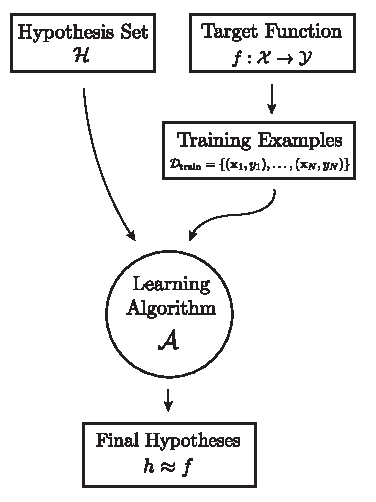
\includegraphics[width=0.9\textwidth]{figures/learning_problem/learning_problem.pdf}
  \caption[blabla.]
    {bla.
    }
  \label{fig:ml:learning_problem}
\end{marginfigure}



$\mathcal{X}$ \\
$\mathcal{Y}$ \\
$X \in \mathcal{X}$ \\
$(X, Y) \in \left(\mathcal{X} \times \mathcal{Y} \right)$ \\
$S = \{ (X_1, Y_1), \ldots, (X_n, Y_n) \}$ \\
$h: \mathcal{X} \mapsto \mathcal{Y}$ \\
$\mathcal{H} = \left\{h_1, h_2, \ldots, h_M  \right\}$ \\
$\ell(Y', Y)$ \\
$\hat{L}(h, S) = \frac{1}{2} \sum_{i=1}^{n} \ell(h(X_i, Y_i))$ \\
$L(h) = \mathbb{E} \left[\ell(h(X), Y) \right]$ \\
$\mathbb{P} \left[ |\nu-\mu| > \epsilon \right] \le 2 e^{-2\epsilon^2 N} \quad \text{for any } \epsilon > 0$  \\
$\mathbb{P} \left[ |E_\text{in}(g)-E_{out}(g)| > \epsilon \right] \le 2 M e^{-2\epsilon^2 N} \quad \text{for any } \epsilon > 0$  \\
$E_\text{out}(g) \le E_{in}(g) + \sqrt{\frac{1}{2N} \ln \frac{2M}{\delta}}$ \\ %  generalization bound
$E_\text{out}(g) \le E_{in}(g) + \sqrt{\frac{8}{2N} \ln \frac{4 m_\mathcal{H}(2N)}{\delta}}$ \\ % VC generalization bound
$E_\text{out}(g^{(\mathcal{D})}) = \mathbb{E}_\mathbf{x} \left[ \left(g^{(\mathcal{D})}(\mathbf{x}) - f(\mathbf{x}) \right)^2  \right]$ % out of sample error, bias-variance

$$\mathbb{E}_\mathcal{D} \left[ E_\text{out} \left( g^{\mathcal{D}} \right) \right] = \
\mathbb{E}_\mathbf{x} \biggl[\
\underbrace{\mathbb{E}_\mathcal{D} \left[ g^{\mathcal{D}}\left(\mathbf{x}\right)\right] - \bar{g}\left(\mathbf{x}\right)^2}_{\
\mathbb{E}_\mathcal{D} \left[g^{\mathcal{D}}\left(\mathbf{x}\right)\right] - \bar{g}\left(\mathbf{x}\right)^2} \
+ \underbrace{\bar{g}\left(\mathbf{x}\right)^2 - 2 \bar{g}\left(\mathbf{x}\right)f(\mathbf{x}) + f(\mathbf{x})^2}_{\
\left(\bar{g}(\mathbf{x}) - f(\mathbf{x}) \right)^2} \biggr]$$ \\

$$\prod_{n=1}^{N} P\left( y_n | x_n \right)$$ \\

$$\phi_i = \sum_{S \subseteq N \backslash \{i\}} \frac{|S|!(M-|S|-1)!}{M!} \left[ f_x(S \cup \{i\}) - f_x(S) \right]  $$

$$ g(z') = \phi_0 + \sum_{i=1}^{M} \phi_i {z'}_i $$


\begin{marginfigure}
  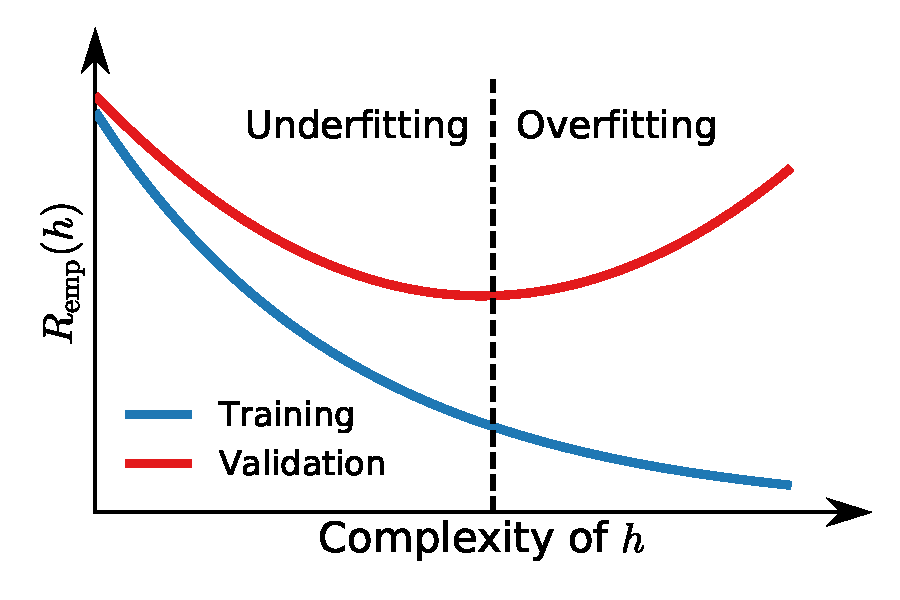
\includegraphics[width=0.9\textwidth]{figures/overfitting/overfitting_1.pdf}
  \caption[Illustration of the empirical risk as a function of model complexity.]
    {Illustration of the empirical risk as a function of model complexity. The \textcolor{blue}{training error} is shown in blue and \textcolor{red}{validation error} in red.
    }
  \label{fig:ml:empirical_risk}
\end{marginfigure}


\begin{figure}
  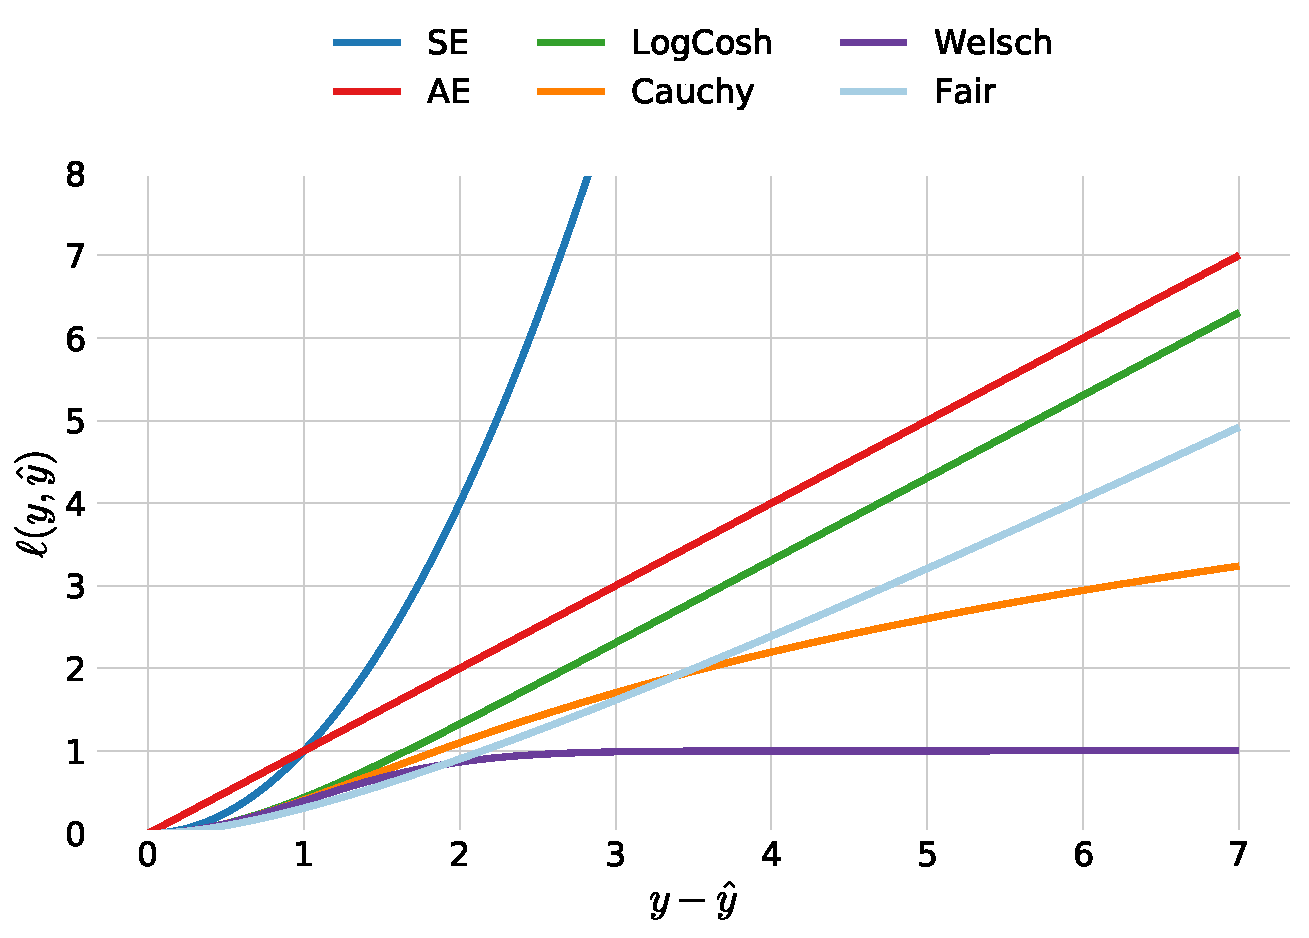
\includegraphics[width=0.9\textwidth]{figures/objective_functions/objective_functions.pdf}
  \caption[Comparison of different objective functions.]
    {Comparison of the the six objective functions MSE, MAE, LogCosh, Cauchy, Welsch, and Fair as a function of $|z|$. In the plot \textcolor{blue}{MSE} is shown in blue, \textcolor{red}{MAE} in red, \textcolor{green}{LogCosh} in green, \textcolor{orange}{Cauchy} in orange, \textcolor{purple}{Welsch} in purple, and \textcolor{light-blue}{Fair} in light blue. For the Cauchy and Welsch functions $C$ is set to 1 and for the Fair function $c$ is set to 1. For a zoom in of the inner region where $|z|<2$ see \figref{fig:ml:objective_funcs_zoom}. 
    }
  \label{fig:ml:objective_funcs}
\end{figure}


\begin{marginfigure}
  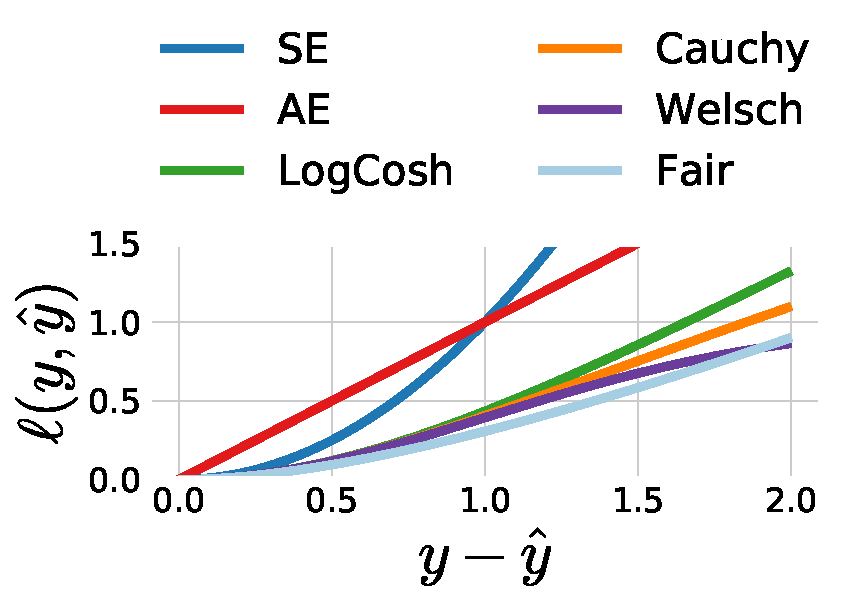
\includegraphics[width=0.9\textwidth]{figures/objective_functions/objective_functions_zoom.pdf}
  \caption[Comparison of different objective functions zoom in.]
    {Zoom in of \figref{fig:ml:objective_funcs}. 
    }
  \label{fig:ml:objective_funcs_zoom}
\end{marginfigure}





\begin{figure}
  \includestandalone[width=0.9\textwidth]{figures/decision_tree/decision_tree}%     without .tex extension
  % or use \input{mytikz}
  \caption{My TikZ picture 1}
  \label{fig:tikz:decision_tree_1}
\end{figure}

\begin{marginfigure}[-4cm]
  \includestandalone[width=0.9\textwidth]{figures/decision_tree/decision_tree}%     without .tex extension
  % or use \input{mytikz}
  \caption{My TikZ picture 2}
  \label{fig:tikz:decision_tree_2}
\end{marginfigure}



\begin{figure}
  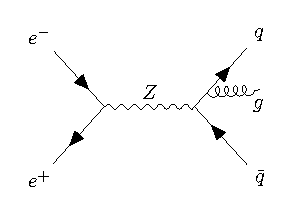
\includegraphics[width=0.9\textwidth]{figures/feynman_diagrams/eeZqqg.pdf}
  \caption[Feynman diagram for the jet production at LEP][6pt]{Feynman diagram showing the $e^+ e^- \rightarrow Z^0$ production at LEP. The $Z^0$ has several decay modes where the $Z \rightarrow q\bar{q}g$ is shown here.}
  \label{fig:feynman_3j_qqg}
  %\zsavepos{pos:textfig}
\end{figure}


\chapter{Housing Prices Analysis}
\label{ch:housing_price_analysis}

\begin{figure}
  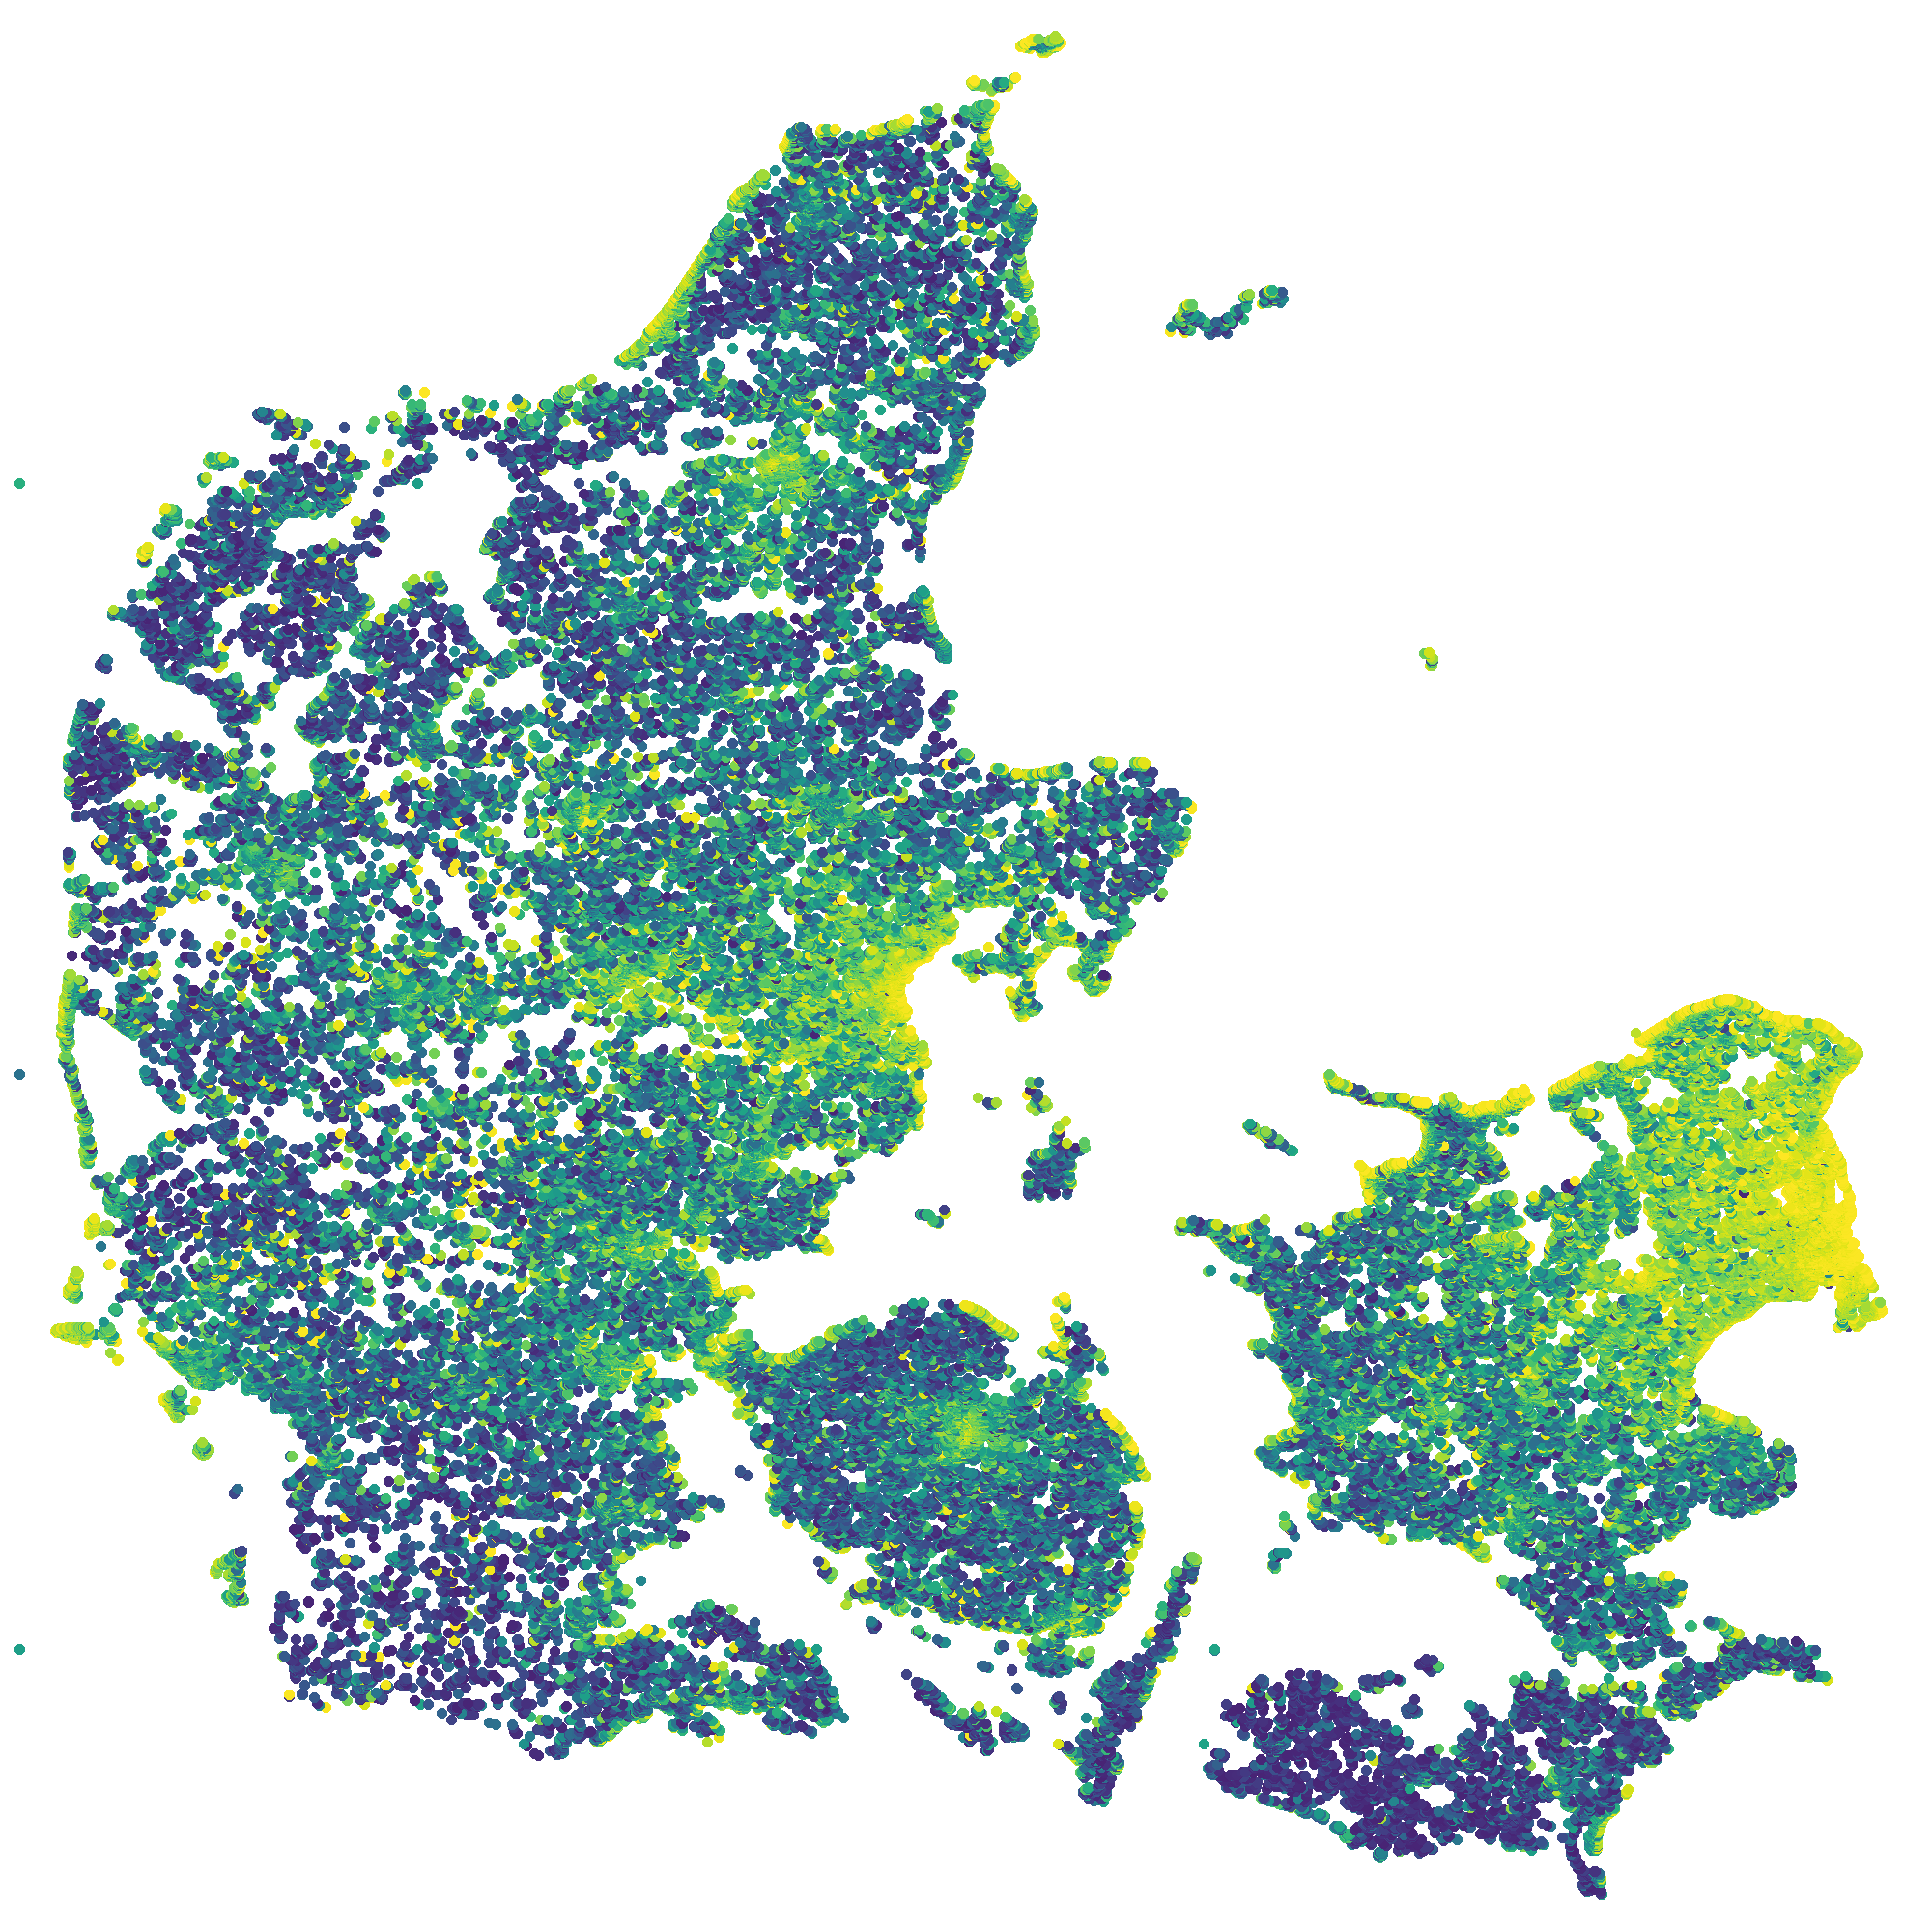
\includegraphics[width=0.9\textwidth, trim=0 0 0 0, clip]{figures/housing/Denmark_Overview_SqmPrice.png}
  \caption[Geographic overview of square meter price in Denmark][6pt]
          {Geographic overview of square meter prices for houses and apartments in Denmark (excluding Bornholm for visual purposes). Notice the strong correlation with the major cities and the shore line. Also notice the three outliers west of Jutland. }
  \label{fig:h:geo_overview}
\end{figure}



\begin{figure}
  \includegraphics[width=0.9\textwidth, page=2]{figures/housing/overview_fig.pdf}
  \caption[Histogram of prices of houses and apartments sold in Denmark][6pt]
          {Histogram of prices of houses and apartments sold in Denmark.}
  \label{fig:h:price_overview}
\end{figure}


\begin{figure*}[htb]
  \centering
  
  \vspace*{-\abovecaptionskip}
  
  \subfloat[\label{fig:h:variable_overview_a}]{\qquad}
  \includegraphics[width=0.4\textwidth, page=2]{figures/housing/overview_fig.pdf}\hfil
  \subfloat[\label{fig:h:variable_overview_b}]{\qquad}
  \includegraphics[width=0.4\textwidth, page=6]{figures/housing/overview_fig.pdf}

  \subfloat[\label{fig:h:variable_overview_c}]{\qquad}
  \includegraphics[width=0.4\textwidth, page=20]{figures/housing/overview_fig.pdf}\hfil
  \subfloat[\label{fig:h:variable_overview_d}]{\qquad}
  \includegraphics[width=0.4\textwidth, page=23]{figures/housing/overview_fig.pdf}
  
  \caption[Input paramater distributions for the housing prices dataset]{Distributions of the four out of the XXX input variables. Subplot ~\protect\subref{fig:h:variable_overview_a} shows the date of the sale, 
           Subplot ~\protect\subref{fig:h:variable_overview_b} shows the type of sale,
           Subplot ~\protect\subref{fig:h:variable_overview_c} shows the longitude,
           Subplot ~\protect\subref{fig:h:variable_overview_d} shows the area,}
  \label{fig:h:variable_overview}
  
  \vspace{\abovecaptionskip}
\end{figure*}


Outside referencing isn't different: In fig.~\ref{fig:h:variable_overview}: Two images --- fig.~\subref{fig:h:variable_overview_a} shows an "A", fig.~\subref{fig:h:variable_overview_b} shows a "B".



\begin{figure}
  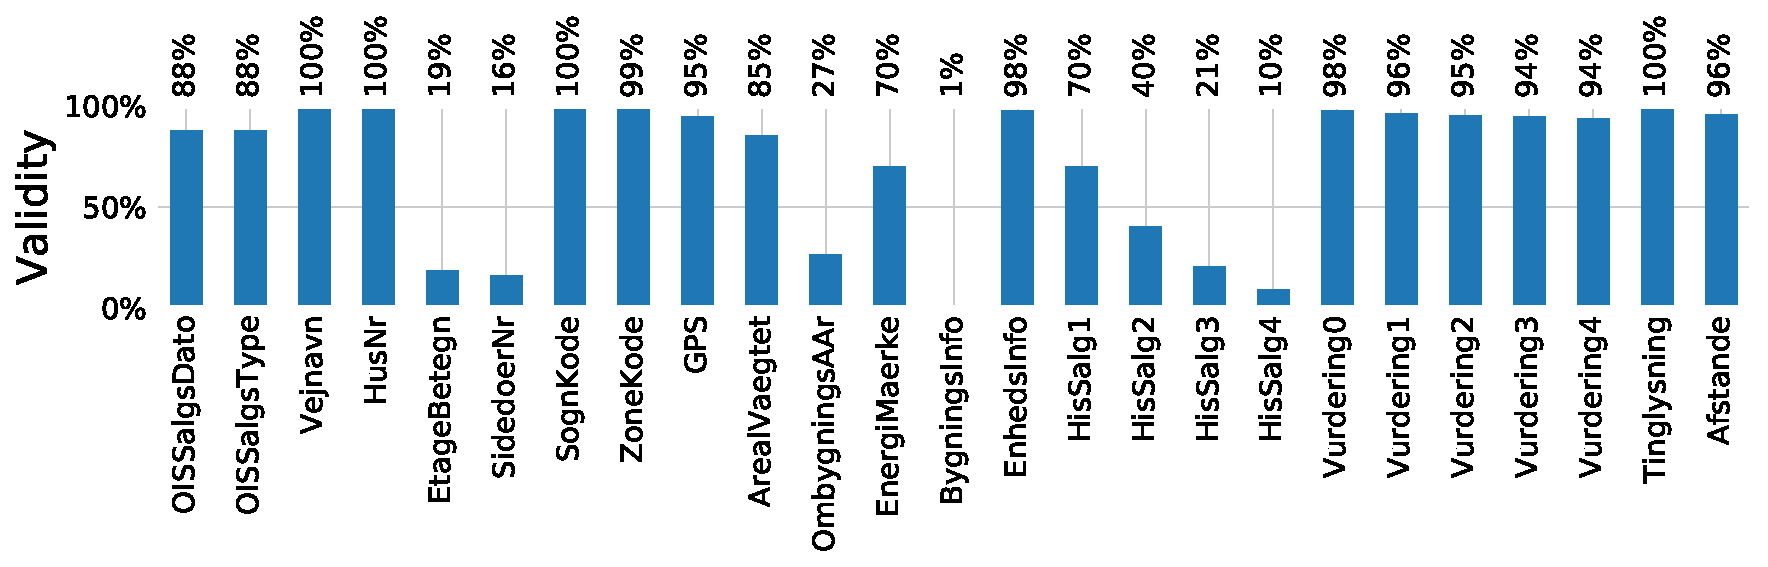
\includegraphics[width=0.9\textwidth, trim=0 0 0 40, clip]{figures/housing/missing_bar.pdf}
  \caption[Percentage of valid counts for each variable][6pt]
          {Percentage of valid counts for each variable grouped together in categories.}
  \label{fig:h:nans}
\end{figure}


\begin{figure}
  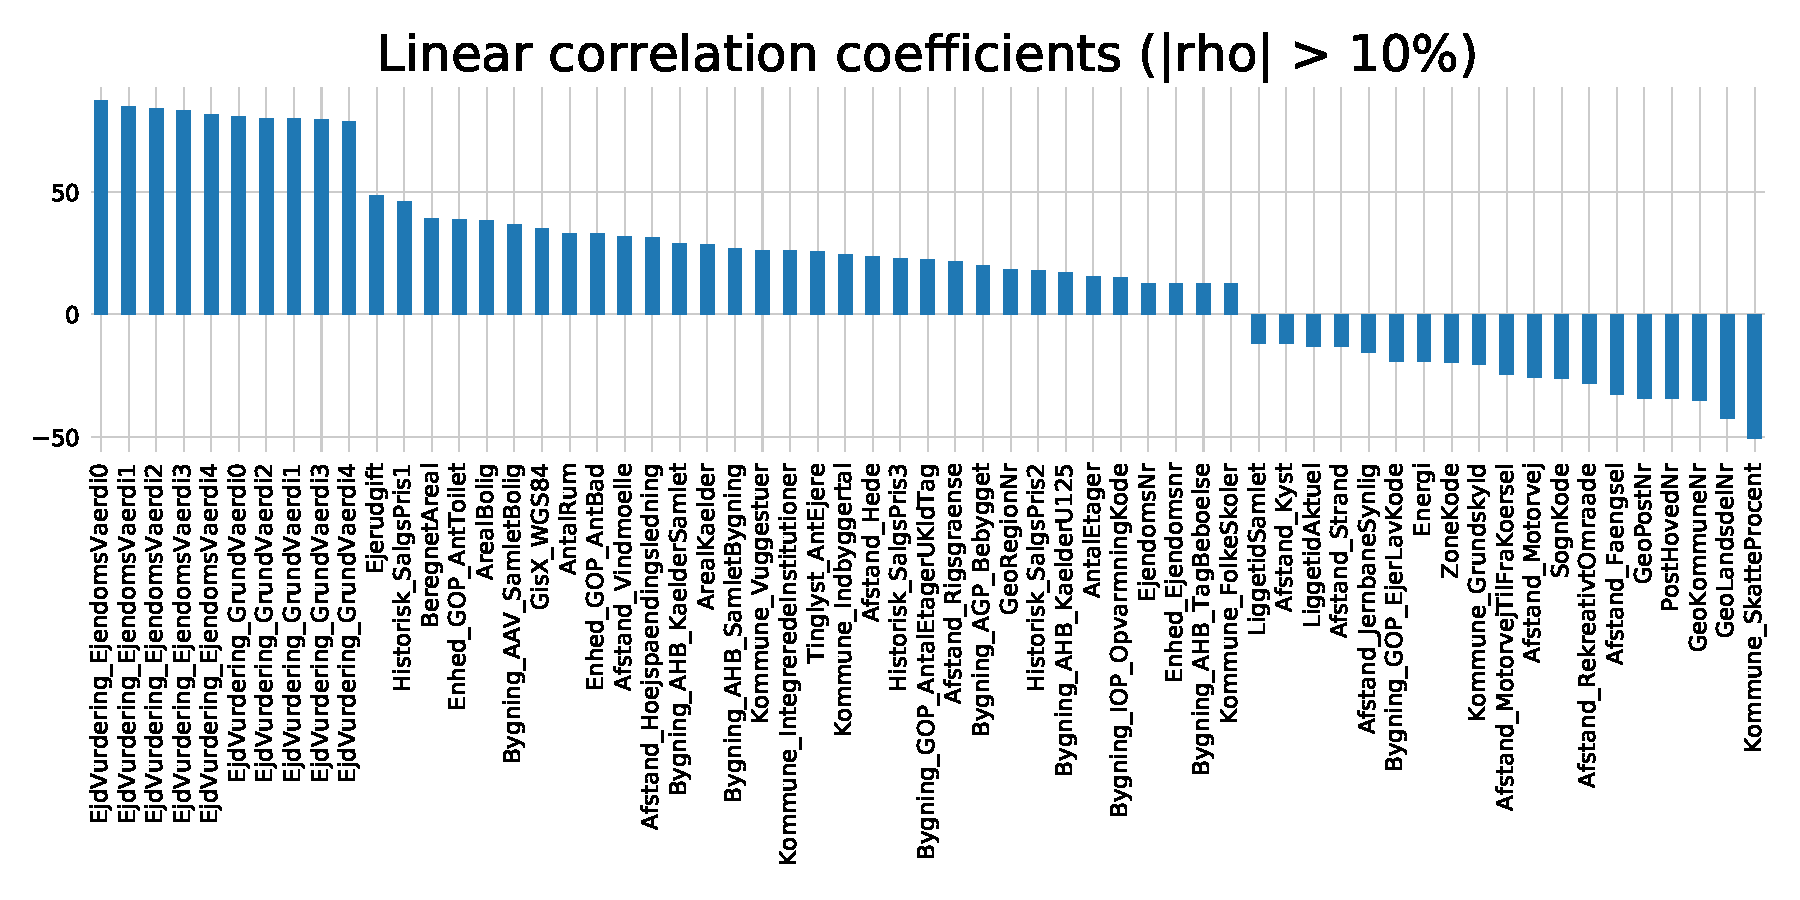
\includegraphics[width=0.9\textwidth, trim=0 0 0 40, clip]{figures/housing/lin_correlation.pdf}
  \caption[Linear correlation between variables and price][6pt]
          {Linear correlation between variables and price for variables where the correlation coefficient $\rho$ is $|\rho| > 10\%$.}
  \label{fig:h:corr_lin}
\end{figure}

\begin{figure}
  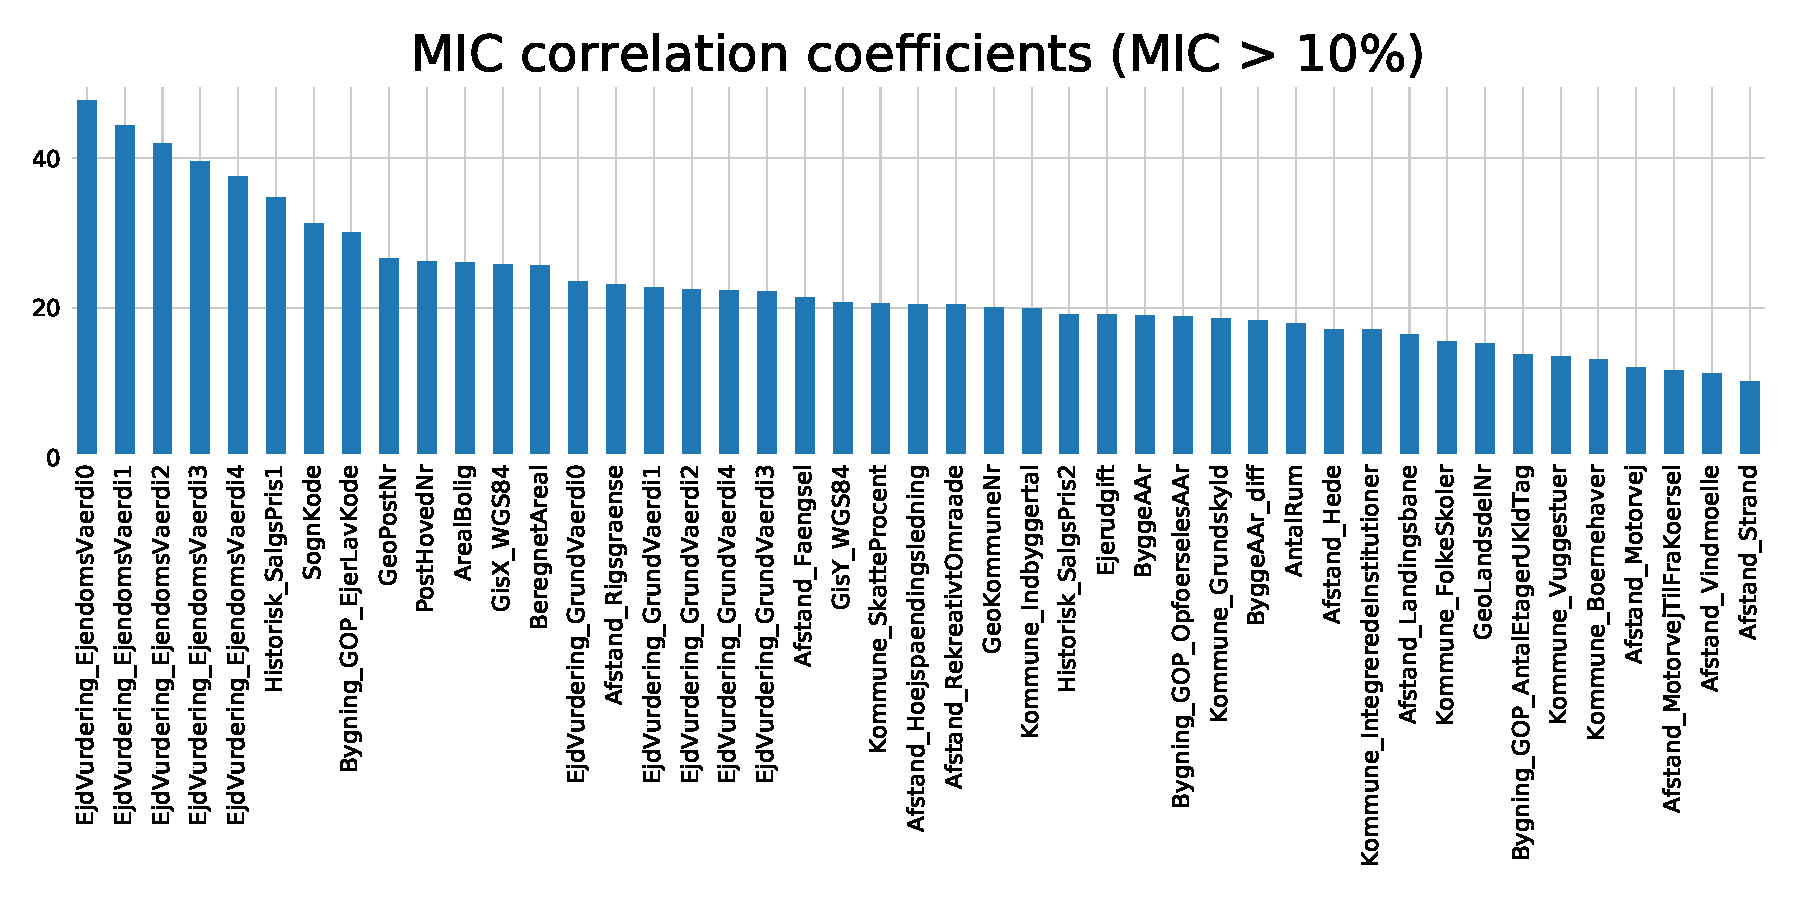
\includegraphics[width=0.9\textwidth, trim=0 0 0 40, clip]{figures/housing/MIC_plot.pdf}
  \caption[Non-linear correlation between variables and price][6pt]
          {Non-linear correlation between variables and price using Maximal Information Coefficient (MIC) for variables where $\text{MIC}>10\%$.}
  \label{fig:h:corr_MIC}
\end{figure}

\begin{figure}
  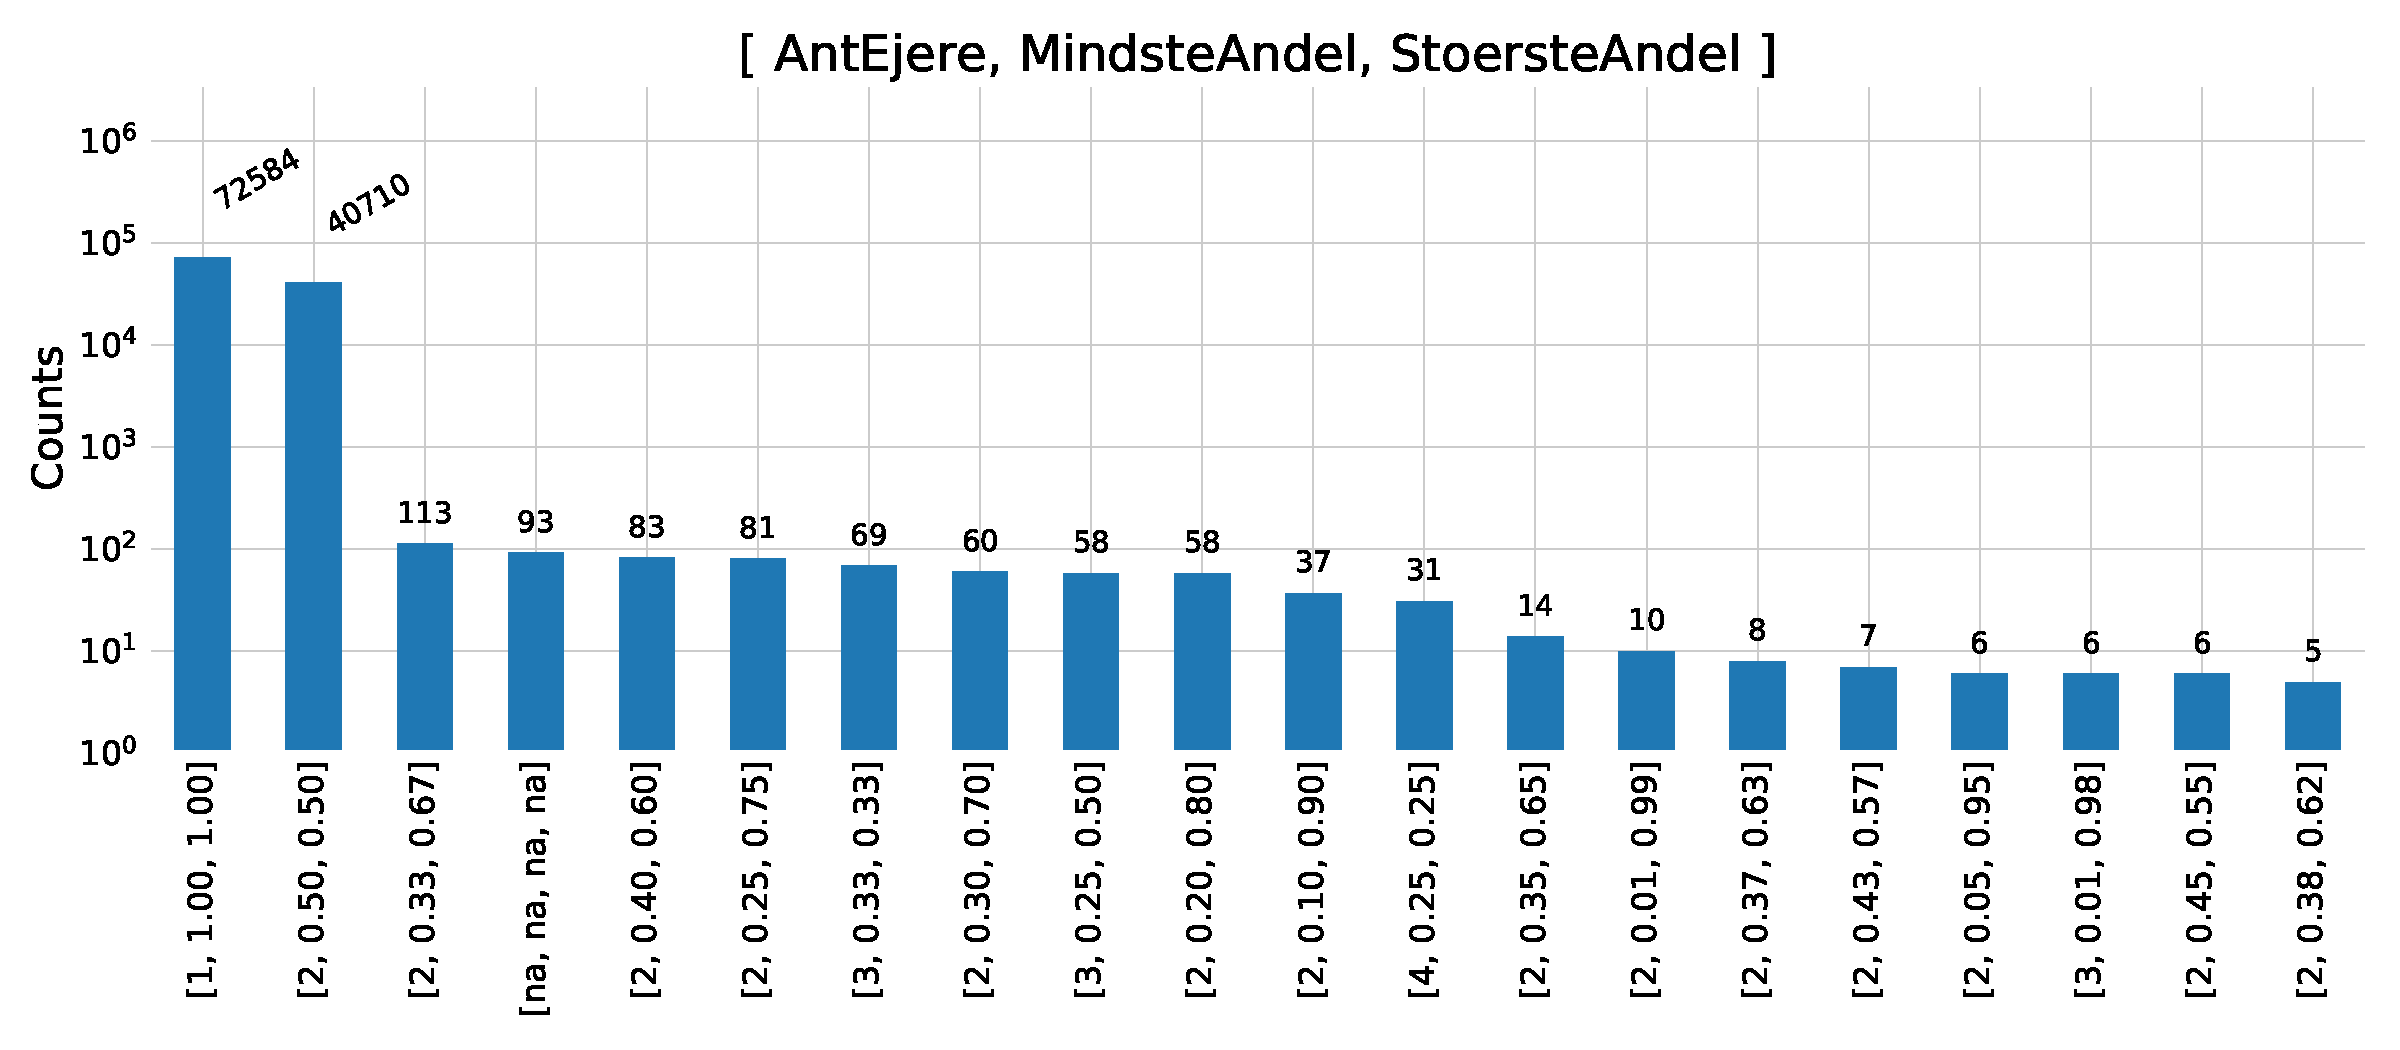
\includegraphics[width=0.9\textwidth]{figures/housing/tinglysning_fig.pdf}
  \caption[Registration of property][6pt]
          {Overview of registration of property as a function of amount of owners (\code{AntEjere}), lowest share (\code{MindsteAndel}) and biggest share (\code{StoersteAndel}) written as \code{[AntEjere, MindsteAndel, StoersteAndel]}.
          }
  \label{fig:h:tinglysning}
\end{figure}



\begin{figure}
  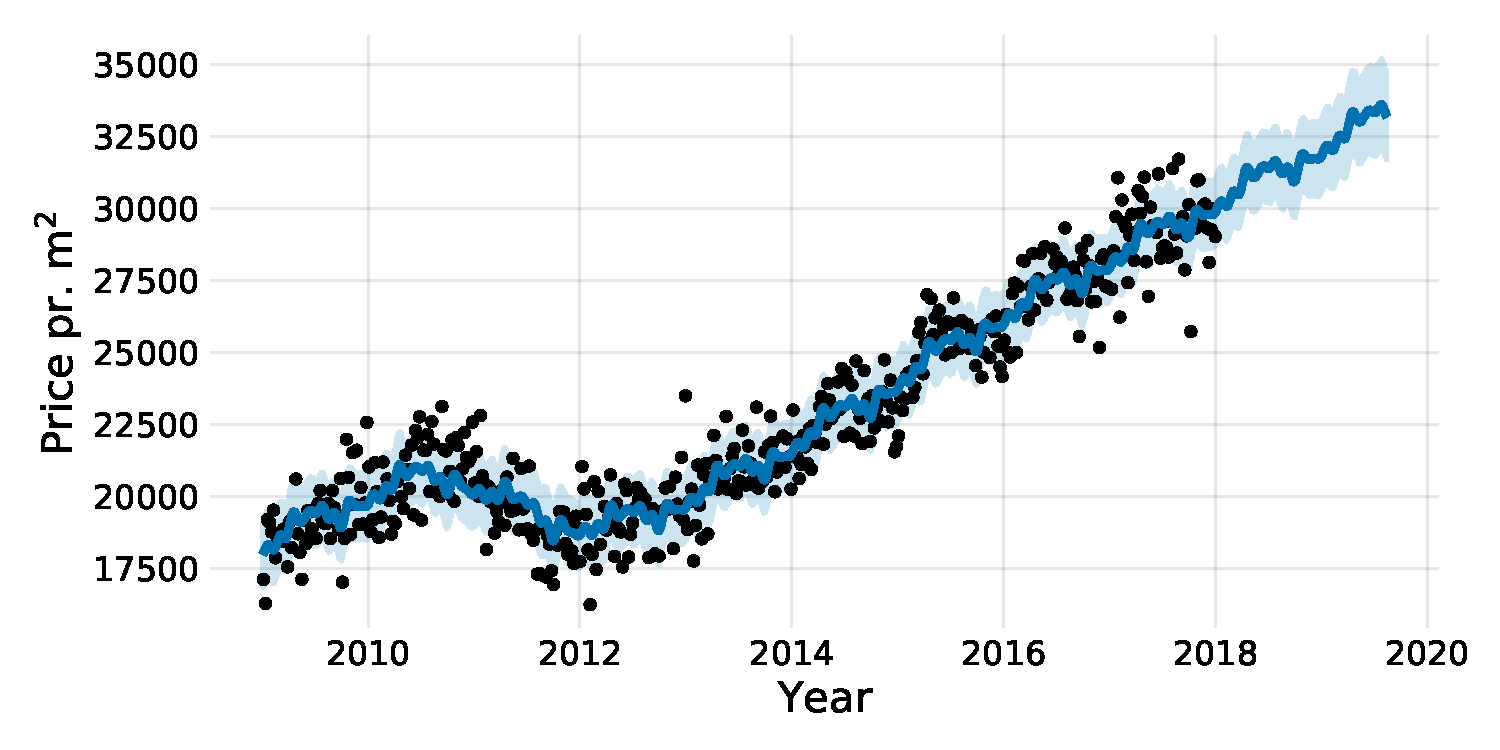
\includegraphics[width=0.9\textwidth]{figures/housing/Ejerlejlighed_v17_cut_all_Ncols_all_prophet_forecast.pdf}
  \caption[Prophet Forecast for apartments][6pt]
          {The predictions of the Facebook Prophet model trained on square meter prices for apartments sold before January 1st, 2018. The data is down-sampled to weekly bins where the median of each week is used as in input to the Prophet model. This can be seen as black dots in the figure. The \textcolor{blue}{model's forecasts} for 2018 and 2019 are shown in blue with a light blue \textcolor{light-blue}{error band} showing the 1-sigma confidence interval.
          }
  \label{fig:h:prophet_forecast}
\end{figure}


\begin{figure}
  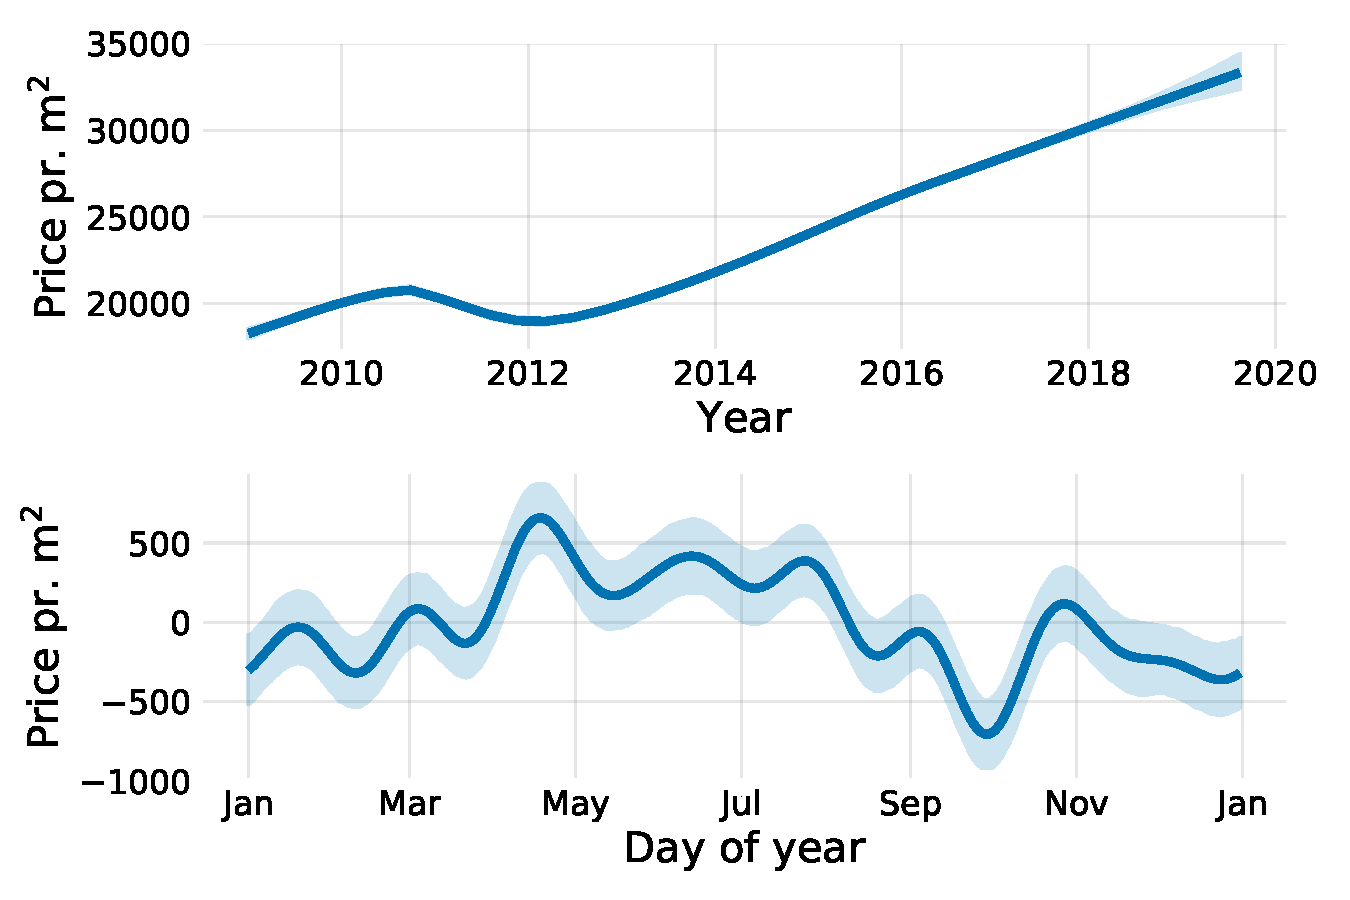
\includegraphics[width=0.9\textwidth]{figures/housing/Ejerlejlighed_v17_cut_all_Ncols_all_prophet_trends.pdf}
  \caption[Prophet Trends][6pt]
          {The trends of the Facebook Prophet model trained on square meter prices for apartments sold before January 1st, 2018. In the top plot is the overall trend as a function of year and in the bottom plot is the yearly variation as a function of day of year. It can be seen that the square meter price is higher during the Summer months compared to the Winter months, however, compared to the overall trend this effect is minor ($<10\%$). 
          }
  \label{fig:h:prophet_trends}
\end{figure}



% \begin{table}[]
  % \begin{tabular}{@{}lllll@{}}

\begin{table}[]
  \begin{tabular}{@{}llrrl@{}}
    \toprule
  Halflife & $\log_{10}$ & $N_\mathrm{trees}$ & Time [$s$]   & MAD    \\ \midrule
  2.5 & True & 210 & 81  & 0.1651 \\
  2.5 & False & 217 & 64  & 0.1791 \\
  5   & True & 209 & 78  & 0.1647 \\
  5   & False & 100 & 41  & 0.1950  \\
  \textbf{10}  & \textbf{True} & \textbf{375} & \textbf{118} & \textbf{0.1563} \\
  10  & False & 411 & 97   & 0.1739 \\
  20  & True & 333 & 106 & 0.1639 \\
  20  & False & 125 & 44  & 0.1925 \\
  $\infty$   & True & 371 & 112 & 0.1596 \\
  $\infty$   & False & 79  & 30  & 0.2062 \\ \bottomrule
  \end{tabular}
  \caption{\label{tab:h:HPO_initial_RMSE}RMSE.}
  \end{table}
  
  \begin{table}[]
  \begin{tabular}{@{}llrrl@{}}
    \toprule
  Halflife & $\log_{10}$ & $N_\mathrm{trees}$ & Time [$s$]   & MAD    \\ \midrule
  2.5 & True & 180 & 57  & 0.1650  \\
  \textbf{2.5} & \textbf{False} & \textbf{682} & \textbf{111} & \textbf{0.1500}   \\
  5   & True & 198 & 62  & 0.1647 \\
  5   & False & 892 & 139 & 0.1514 \\
  10  & True & 244 & 68  & 0.1627 \\
  10  & False & 381 & 65  & 0.1608 \\
  20  & True & 396 & 95  & 0.1612 \\
  20  & False & 302 & 53   & 0.1626 \\
  $\infty$   & True & 239 & 60  & 0.1639 \\
  $\infty$   & False & 303 & 50   & 0.1620  \\ \bottomrule
  \end{tabular}
  \caption{\label{tab:h:HPO_initial_LogCosh}LogCosh.}
  \end{table}
  
  % \begin{table}[]
  % \begin{tabular}{@{}llrrl@{}}
  %   \toprule
  % Halflife & $\log_{10}$ & $N_\mathrm{trees}$ & Time [$s$]   & MAD    \\ \midrule
  % 2.5 & True & 267  & 75  & 0.1866 \\
  % 2.5 & False & 712  & 113 & 0.2794 \\
  % \textbf{5}   & \textbf{True} & \textbf{386}  & \textbf{91}  & \textbf{0.1843} \\
  % 5   & False & 394  & 60   & 0.2995 \\
  % 10  & True & 88   & 39  & 0.2426 \\
  % 10  & False & 215  & 39  & 0.3668 \\
  % 20  & True & 159  & 51  & 0.2152 \\
  % 20  & False & 604  & 89  & 0.3340  \\
  % $\infty$   & True & 326  & 82  & 0.1982 \\
  % $\infty$   & False & 1146 & 161 & 0.2963 \\ \bottomrule
  % \end{tabular}
  % \caption{\label{tab:h:HPO_initial_Cauchy}Cauchy.}
  % \end{table}
  
  % \begin{table}[]
  % \begin{tabular}{@{}llrrl@{}}
  %   \toprule
  % Halflife & $\log_{10}$ & $N_\mathrm{trees}$ & Time [$s$]   & MAD    \\ \midrule
  % 2.5    & True & 227  & 69  & 0.1973 \\
  % 2.5 & False & 621  & 99  & 0.4257 \\
  % 5   & True & 205  & 61  & 0.2128 \\
  % 5   & False & 320  & 53  & 0.4048 \\
  % \textbf{10}  & \textbf{True} & \textbf{286}  & \textbf{78}  & \textbf{0.1960}  \\
  % 10  & False & 1109 & 153 & 0.4045 \\
  % 20  & True & 171  & 53  & 0.2069 \\
  % 20  & False & 809  & 108  & 0.3698 \\
  % $\infty$   & True & 215  & 63  & 0.2194 \\
  % $\infty$   & False & 558  & 81  & 0.3933 \\ \bottomrule
  % \end{tabular}
  % \caption{\label{tab:h:HPO_initial_Welsch}Welsch.}
  % \end{table}
  
  % \begin{table}[]
  % \begin{tabular}{@{}llrrl@{}}
  %   \toprule
  % Halflife & $\log_{10}$ & $N_\mathrm{trees}$ & Time [$s$]   & MAD    \\ \midrule
  % 2.5 & True & 209 & 62 & 0.1631 \\
  % 2.5 & False & 170 & 37 & 0.1702 \\
  % 5   & True & 360 & 94 & 0.1623 \\
  % 5   & False & 252 & 49 & 0.1698 \\
  % \textbf{10}  & \textbf{True} & \textbf{368} & \textbf{93}  & \textbf{0.1574} \\
  % 10  & False & 322 & 53 & 0.1711 \\
  % 20  & True & 257 & 66 & 0.1614 \\
  % 20  & False & 313 & 50 & 0.1706 \\
  % $\infty$   & True & 351 & 85 & 0.1602 \\
  % $\infty$   & False & 360 & 57 & 0.1740  \\ \bottomrule
  % \end{tabular}
  % \caption{\label{tab:h:HPO_initial_Fair}Fair.}
  % \end{table}



\begin{figure}
  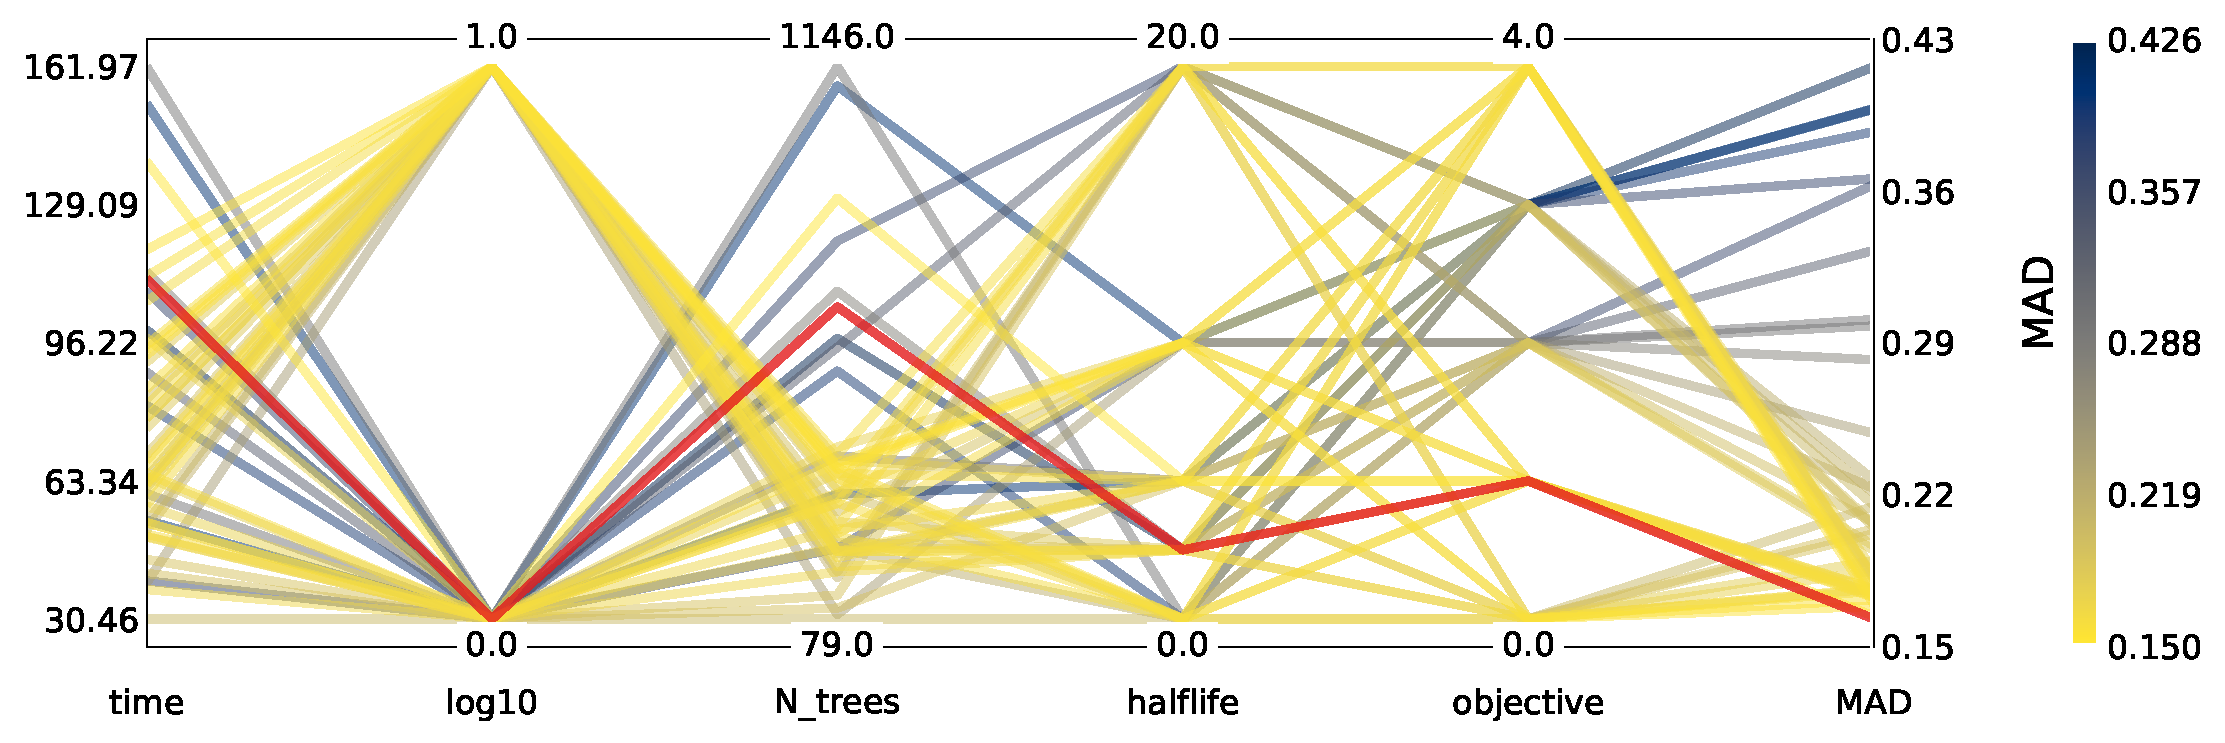
\includegraphics[width=0.95\textwidth, trim=0 0 0 0, clip]{figures/housing/Ejerlejlighed_v17_cut_all_Ncols_all_CV_viz_initial_HPO.pdf}
  \caption[Overview of initial hyperparamater optimization of the housing model for apartments][6pt]
          {Hyperparameter optimization results of the housing model for apartments. The results are shown as parallel coordinates with each hyperparameter along the x-axis and the value of that parameter on the y-axis. Each line is an event in the 4-dimensional space colored according to the performance of that hyperparameter as measured by MAD from \textcolor{viridis-dark}{highest} MAD in dark blue to \textcolor{viridis-light}{lowest} AUC in yellow. The \textcolor{red}{single best hyperparameter} is shown in red. For the hyperparamater \code{log10} \code{0} means False and \code{1} means True, for \code{objektive} the functions RMSE (0), LogCosh (1), Cauchy (2), Welsch (3), and Fair (4) are mapped to the integers in the parentheses.   
          } 
  \label{fig:h:CV_res_parallel_coords}
\end{figure}



\begin{figure}
  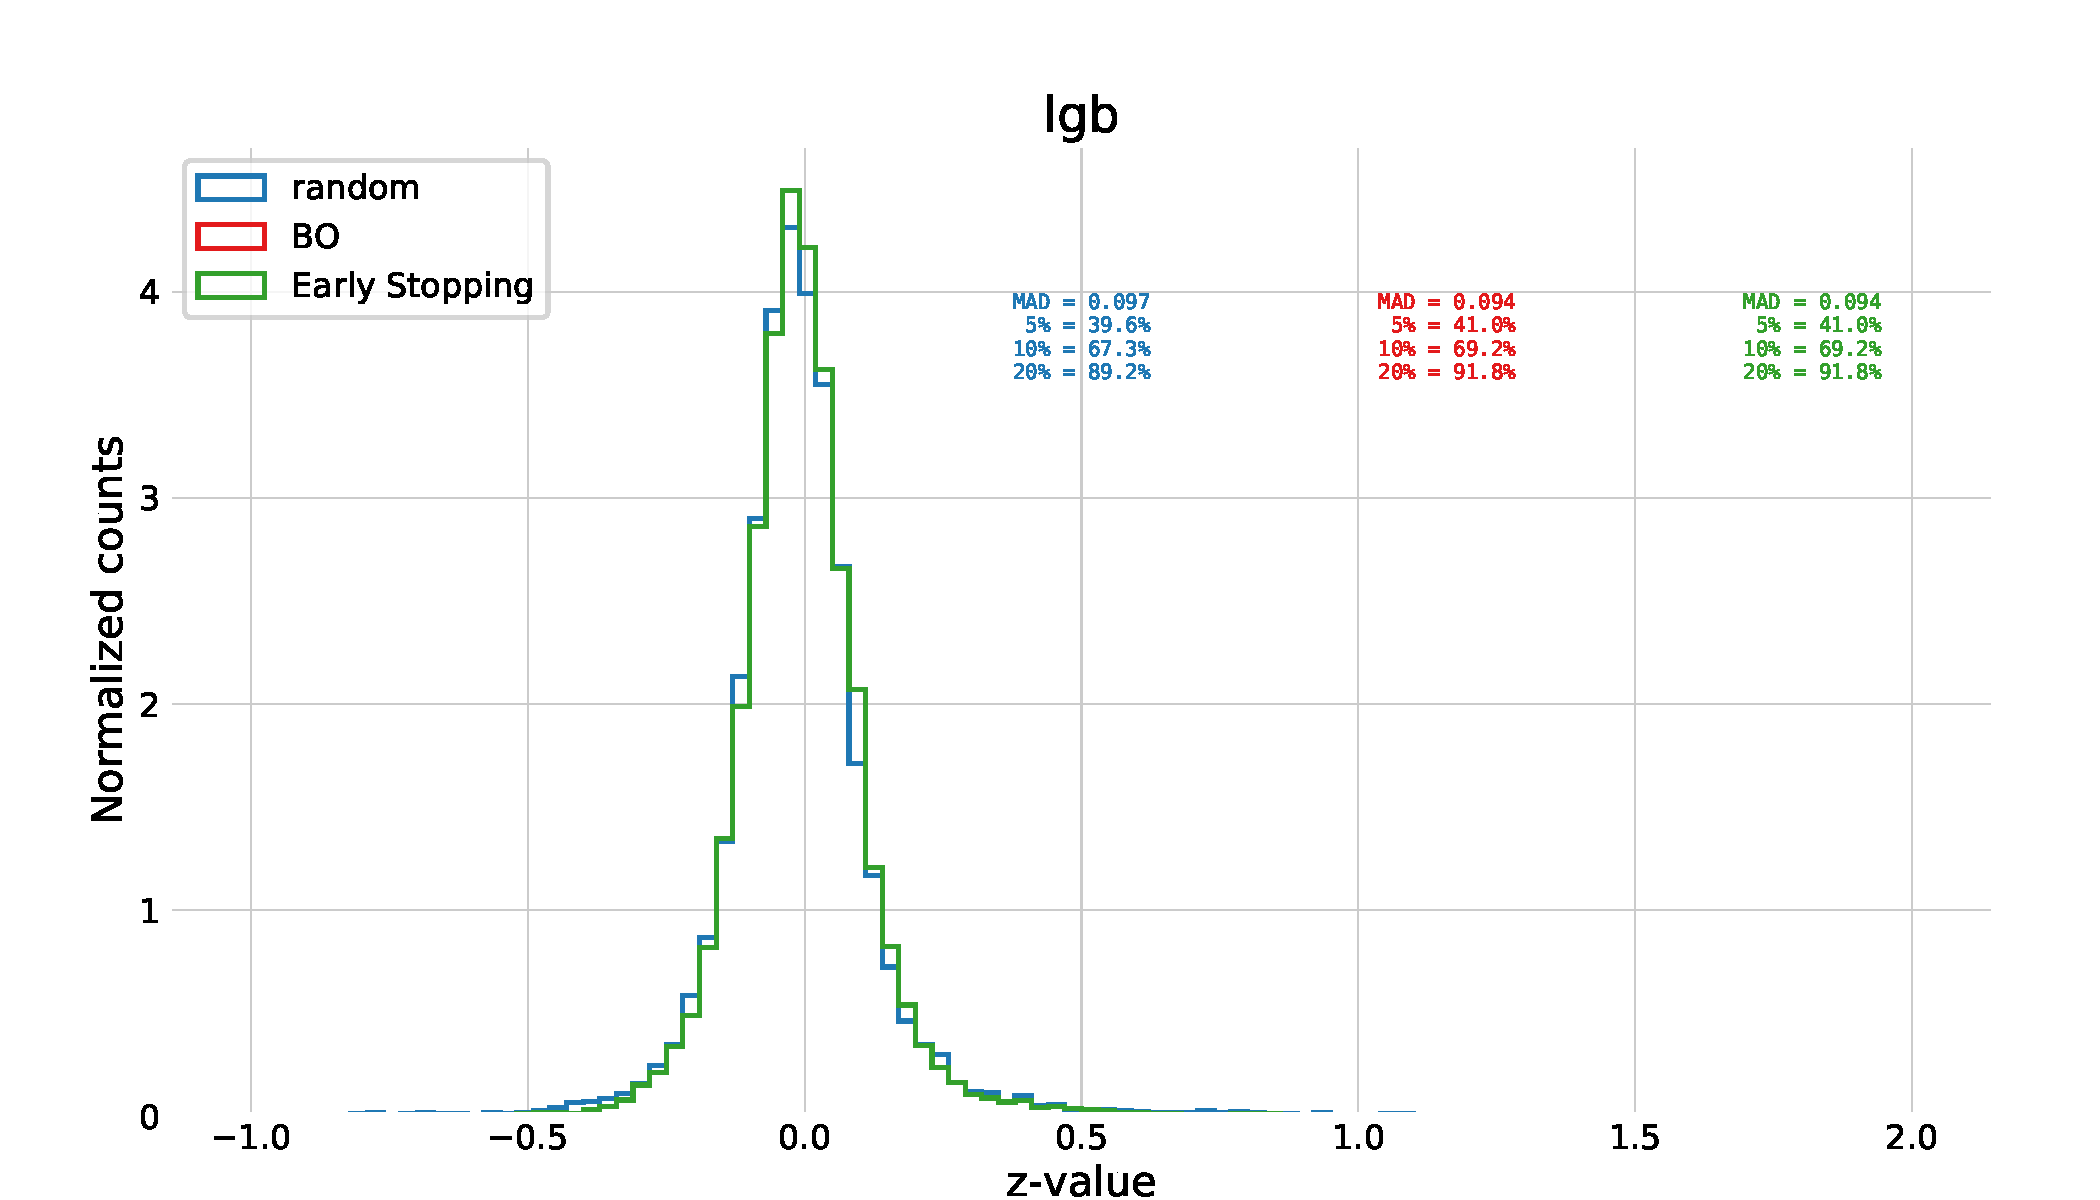
\includegraphics[width=0.9\textwidth, trim=0 0 0 70, clip]{figures/housing/Ejerlejlighed_v17_cut_all_Ncols_all_lgb_z_hist_metrics.pdf}
  \caption[Performance of LGB-model on apartment prices][6pt]
          {Histogram of $z$-values of the LGB-model trained on apartments. The performance after hyperparameter optimization (HPO) using \textcolor{blue}{Random Search} (RS) is shown in blue, for \textcolor{red}{Bayesian Optimization} (BO) in red. After finding the best model, BO in this case, the model is retrained using \textcolor{green}{early stopping}, the performance of which is shown in green.}
  \label{fig:h:performance_lgb}
\end{figure}


\begin{figure}
  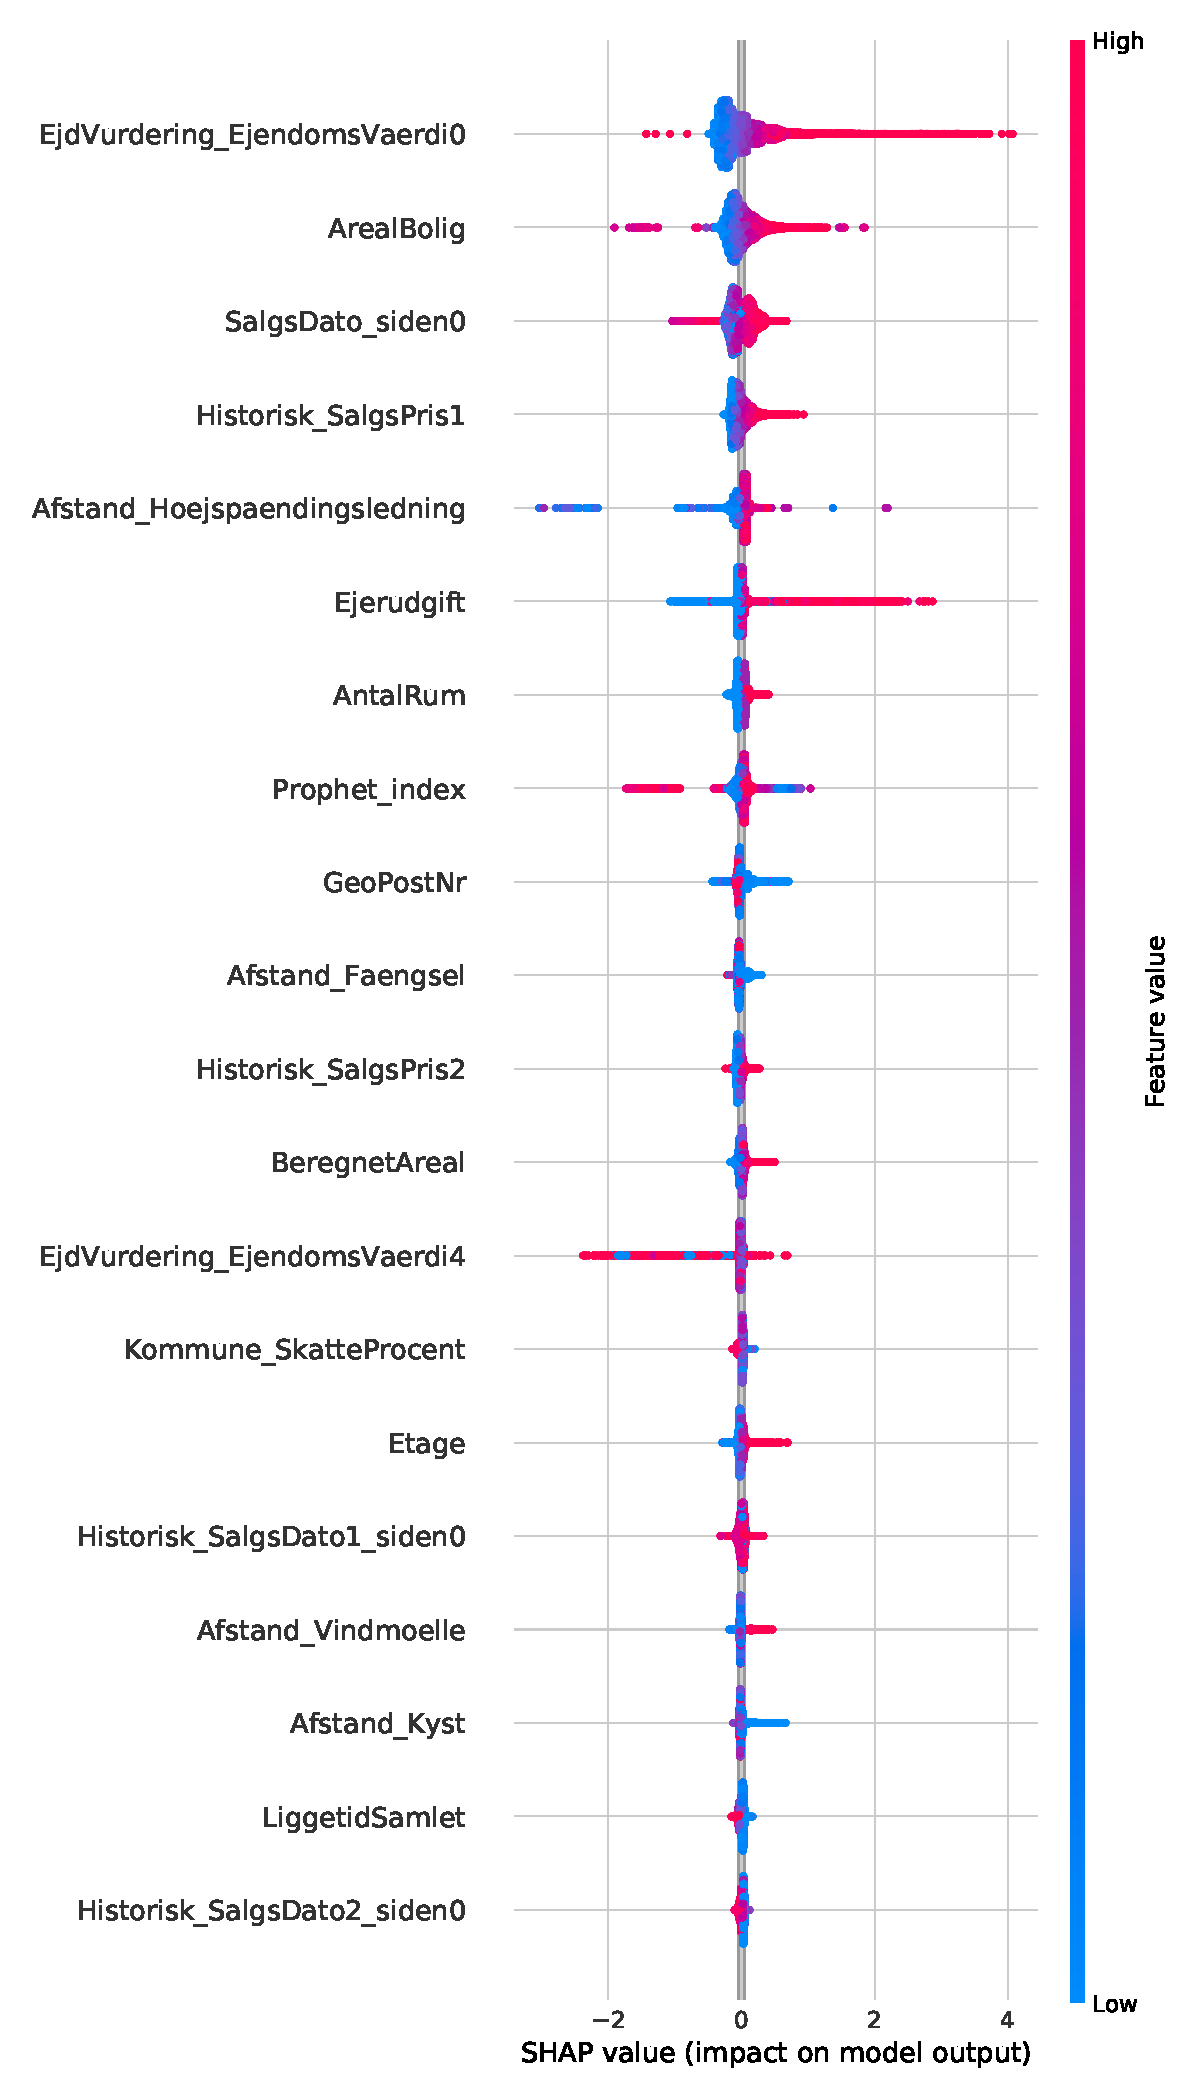
\includegraphics[width=0.9\textwidth, trim=0 0 0 1, clip]{figures/housing/Ejerlejlighed_v17_cut_all_Ncols_all_lgb_tight_SHAP_vals_summary.pdf}
  \caption[Feature importance of apartments prices using LGB][6pt]
          {Feature importance of apartment prices using the LGB-model. The feature importance is measured using SHAP-values. The variables are sorted top to bottom according to their overall feature importance, i.e. the previous public property valuation \code{EjdVurdering_EjendomdsVaerdi0} is the most important single feature. Along the x-axis is the impact on model output, in this example the price in XXX. This axes is colored by the value of the feature, from \textcolor{blue}{low} (blue) to \textcolor{red}{high} (red). In this particular example we see that high values of the previous public property valuation has high, positive impact on the model prediction -- exactly as expected. This is exactly opposite the total days on market (DOM) described by the variable \code{LiggetidSamlet} where a high value has a negative impact.  
          } 
  \label{fig:h:shap_overview}
\end{figure}

\begin{figure}
  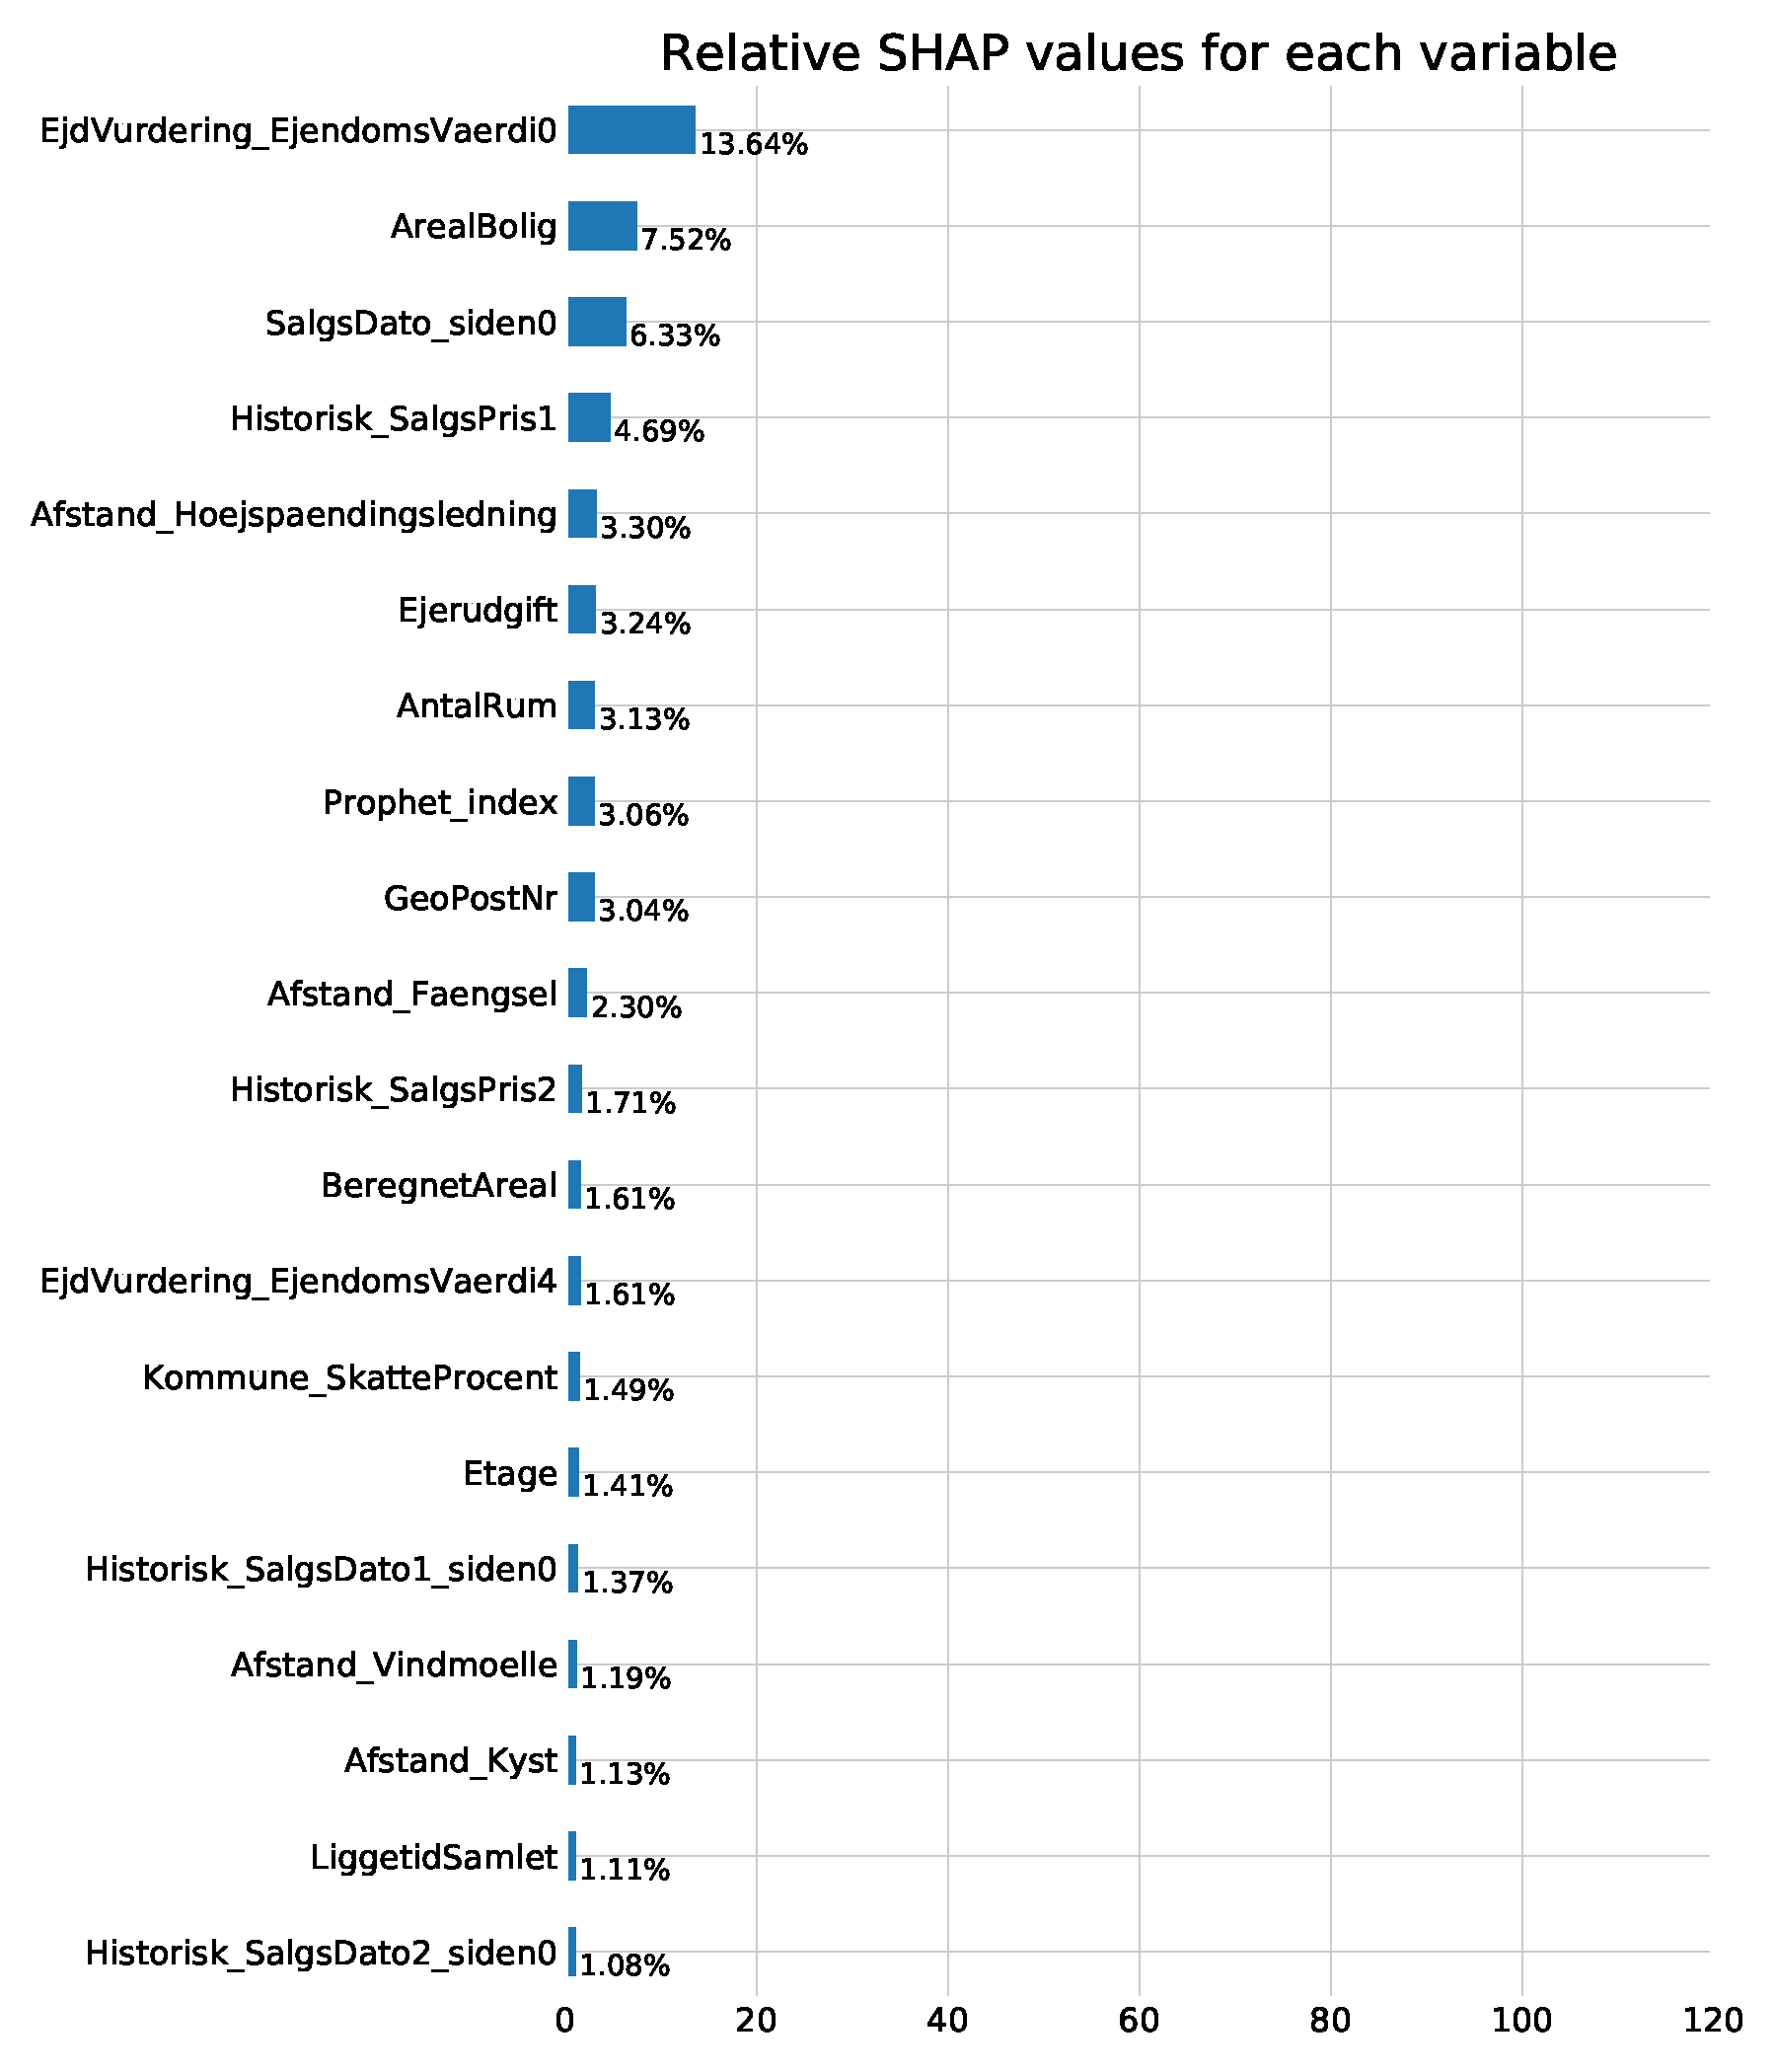
\includegraphics[width=0.9\textwidth, trim=0 0 0 40, clip]{figures/housing/Ejerlejlighed_v17_cut_all_Ncols_all_lgb_tight_SHAP_vals_summary_all.pdf}
  \caption[Total feature importance of apartment prices using LGB][6pt]
          {Total feature importance of apartment prices using the LGB-model. The total feature importance is measured using SHAP-values, more specifically the mean of the absolute SHAP-values for each variable. This allows a ranking of all of the features ordered after the total importance. Here the total feature importance is scaled such that they sum to 1 when summing over all variables. The absolute total feature importance is in itself not important, but the relative values indicate the difference in feature importance. 
          } 
  \label{fig:h:shap_overview_total}
\end{figure}


\begin{figure}
  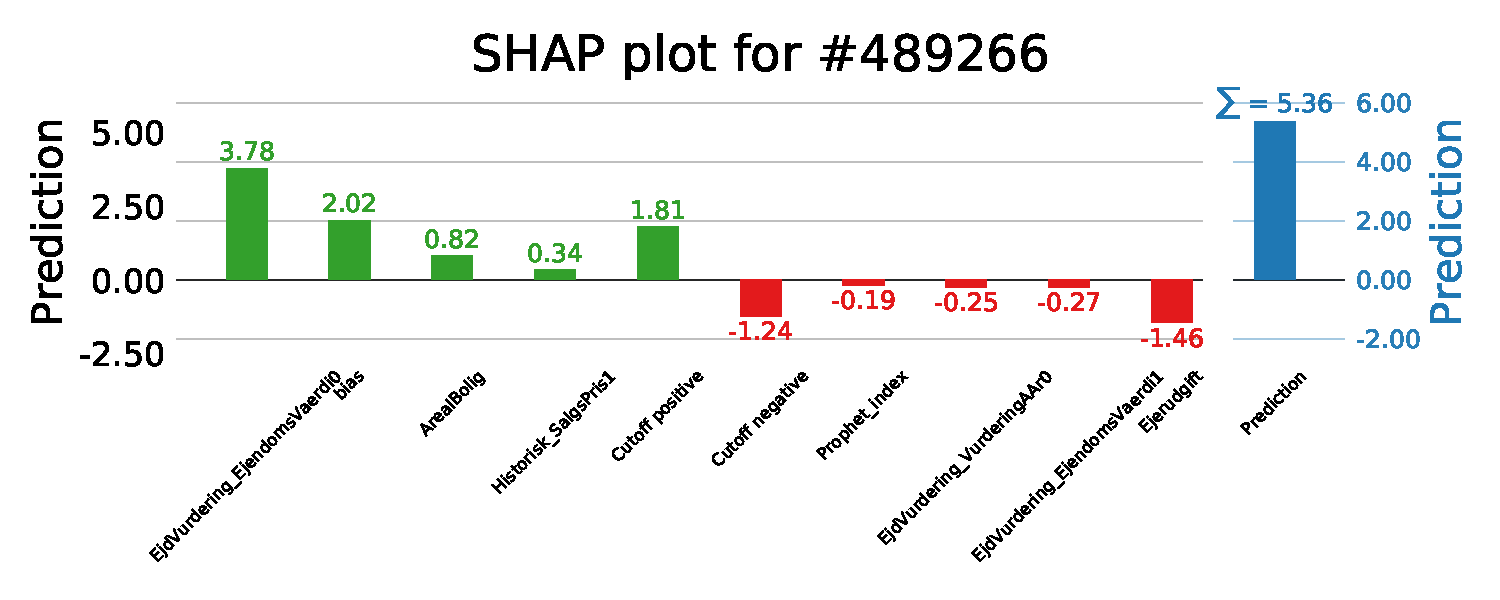
\includegraphics[width=0.95\textwidth, trim=0 0 0 40, clip]{figures/housing/Ejerlejlighed_v17_cut_all_Ncols_all_SHAP_fig_loc=489266.pdf}
  \caption[SHAP Prediction Explanation for apartment][6pt]
          {Model explanation for LGB model for a specific apartment. The bars are the variables in the dataset that the model found most important sorted after their importance for this particular apartment. The bias bar refers to the expected value of the model, which is simply the mean of the training set which acts as the naive prediction baseline. The \q{cutoff positive (negative)} bars are the sum of the remaining positive (negative) values that are not shown. On the right hand side of the plot is the model prediction shown. The model prediction is the sum of all of the bars in the left par (5.36 in this example) calculated in $10^6$ DKK. The \textcolor{red}{negative} values are shown in red, \textcolor{green}{positive} ones in green, and the \textcolor{blue}{prediction value} in blue. 
          } 
  \label{fig:h:shap_single_apartment}
\end{figure}


\begin{figure}
  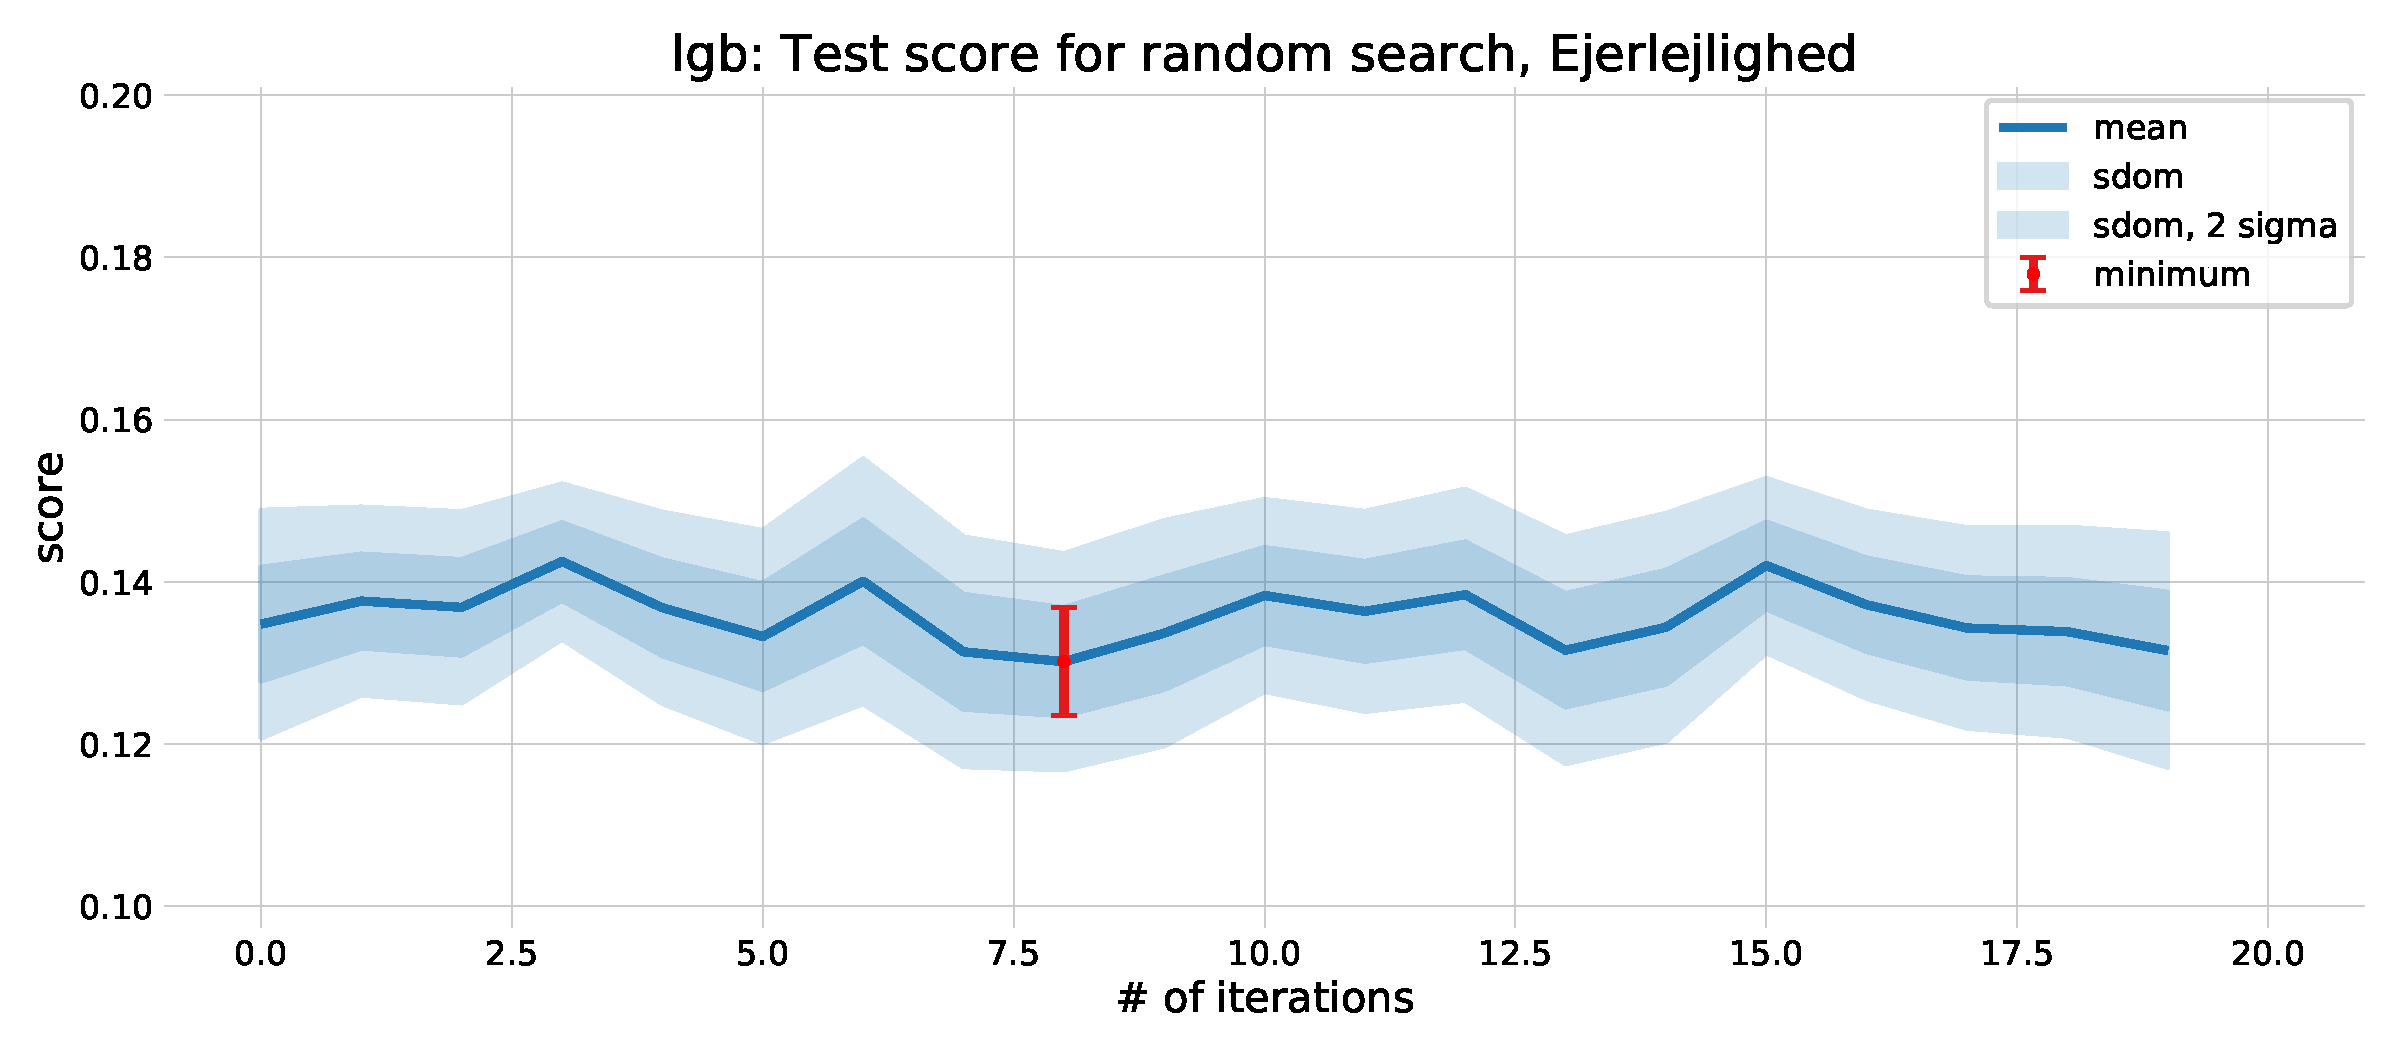
\includegraphics[width=0.9\textwidth, trim=0 0 0 40, clip]{figures/housing/Ejerlejlighed_v17_cut_all_Ncols_all_lgb_score_over_time_random.pdf}
  \caption[Hyperparameter optimization: random search results][6pt]
          {The results of running random search (RS) as hyperparameter optimization (HPO) on apartments using the LGB-model. The \textcolor{red}{minimum (mean) loss} along with its uncertainty is shown in red, the \textcolor{blue}{means} for the different iterations of RS in blue, and as light blue bands are the \textcolor{blue}{one (and two) standard deviation(s) of the means (SDOM)}, all as a a function of iteration number.  
          } 
  \label{fig:h:RS_lgb_apartment}
\end{figure}


\begin{figure}
  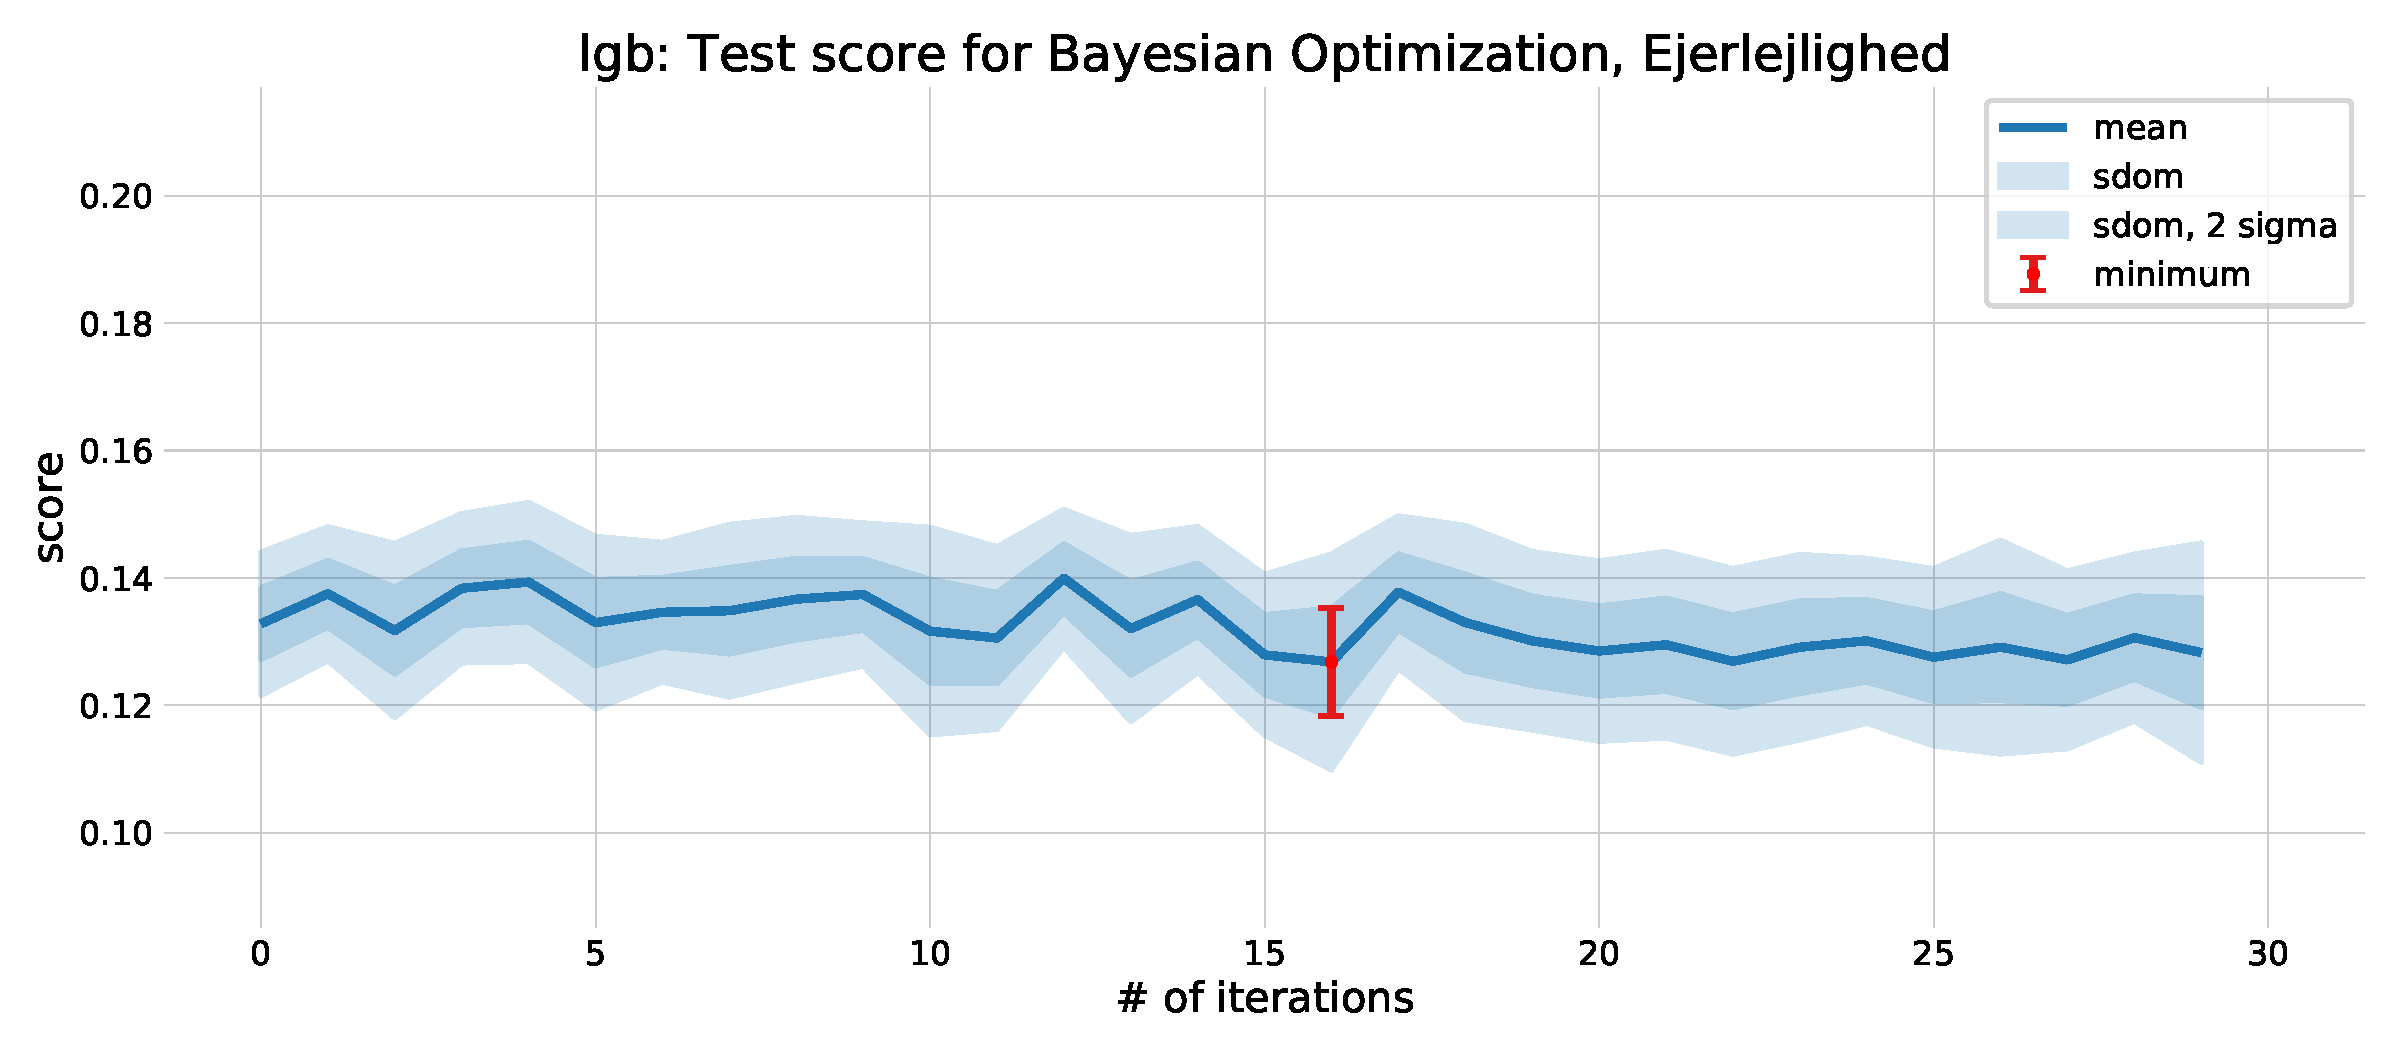
\includegraphics[width=0.9\textwidth, trim=0 0 0 40, clip]{figures/housing/Ejerlejlighed_v17_cut_all_Ncols_all_lgb_score_over_time_BO.pdf}
  \caption[Hyperparameter optimization: Bayesian optimization results][6pt]
          {The results of running Bayesian optimization (BO) as hyperparameter optimization (HPO) on apartments using the LGB-model. The \textcolor{red}{minimum (mean) loss} along with its uncertainty is shown in red, the \textcolor{blue}{means} for the different iterations of RS in blue, and as light blue bands are the \textcolor{blue}{one (and two) standard deviation(s) of the means (SDOM)}, all as a a function of iteration number. The first XXX iterations are run as RS for use as input to the internal optimization algorithm, the last XX iterations are thus the \q{smart} BO guesses.
          } 
  \label{fig:h:BO_lgb_apartment}
\end{figure}


\begin{figure}
  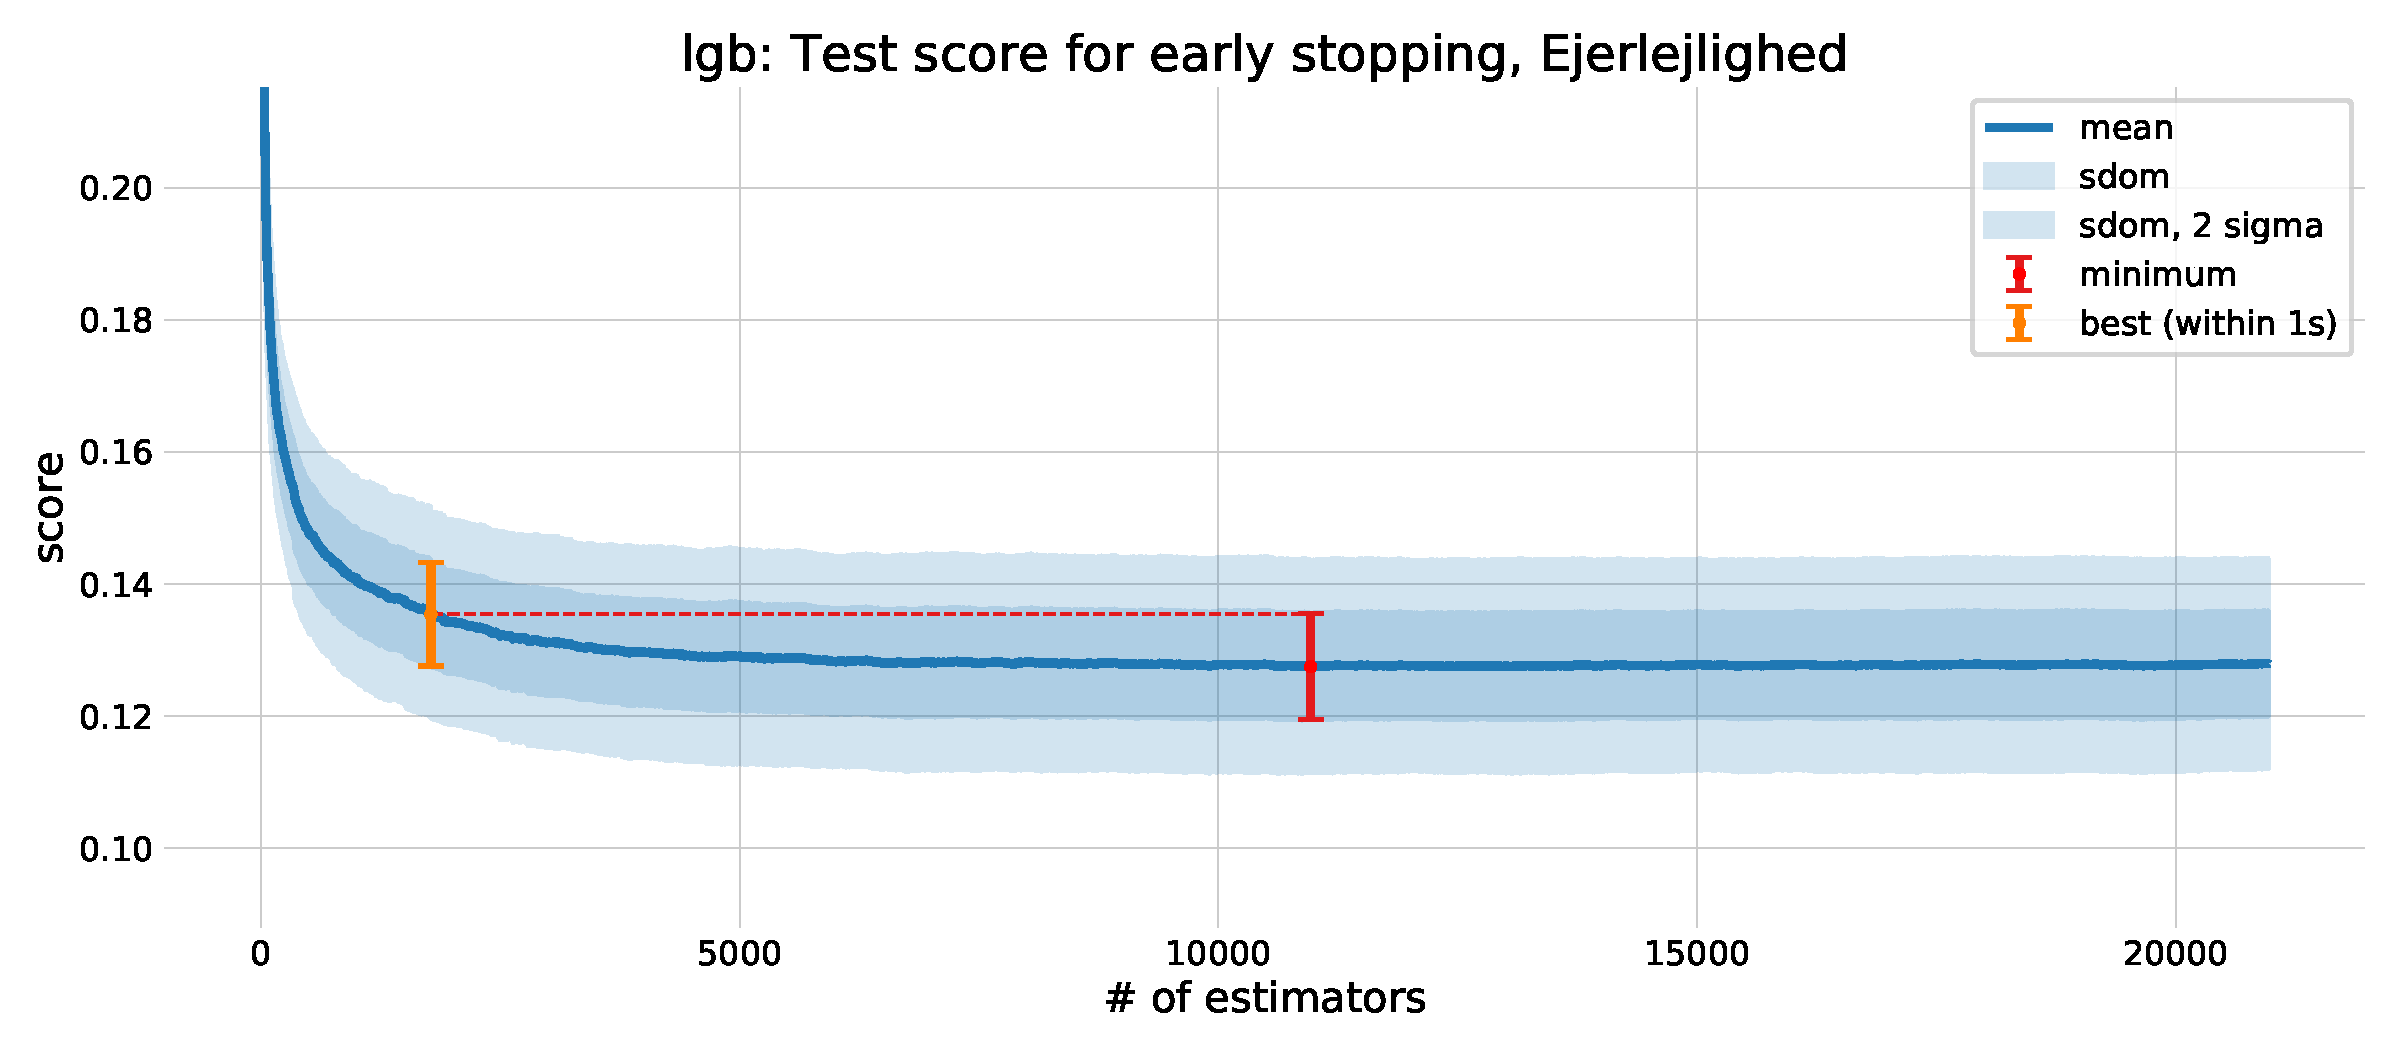
\includegraphics[width=0.9\textwidth, trim=0 0 0 40, clip]{figures/housing/Ejerlejlighed_v17_cut_all_Ncols_all_lgb_early_stopping_fig.pdf}
  \caption[Early Stopping results][6pt]
          {The results of early stopping on apartments using the LGB-model. The \textcolor{red}{minimum (mean) loss} along with its uncertainty is shown in red, the \textcolor{blue}{means} for the different iterations of RS in blue, and as light blue bands are the \textcolor{blue}{one (and two) standard deviation(s) of the means (SDOM)}, all as a a function of number of estimators (trees). In orange the \textcolor{orange}{\q{best} number of estimators} is shown, defined as the lowest number of estimators which are still within 1 SDOM of the minimum value. This leads to a model that has a performance that is within 1 SDOM of the best model, but a lot simpler and faster.  
          } 
  \label{fig:h:early_stopping}
\end{figure}


\begin{figure}
  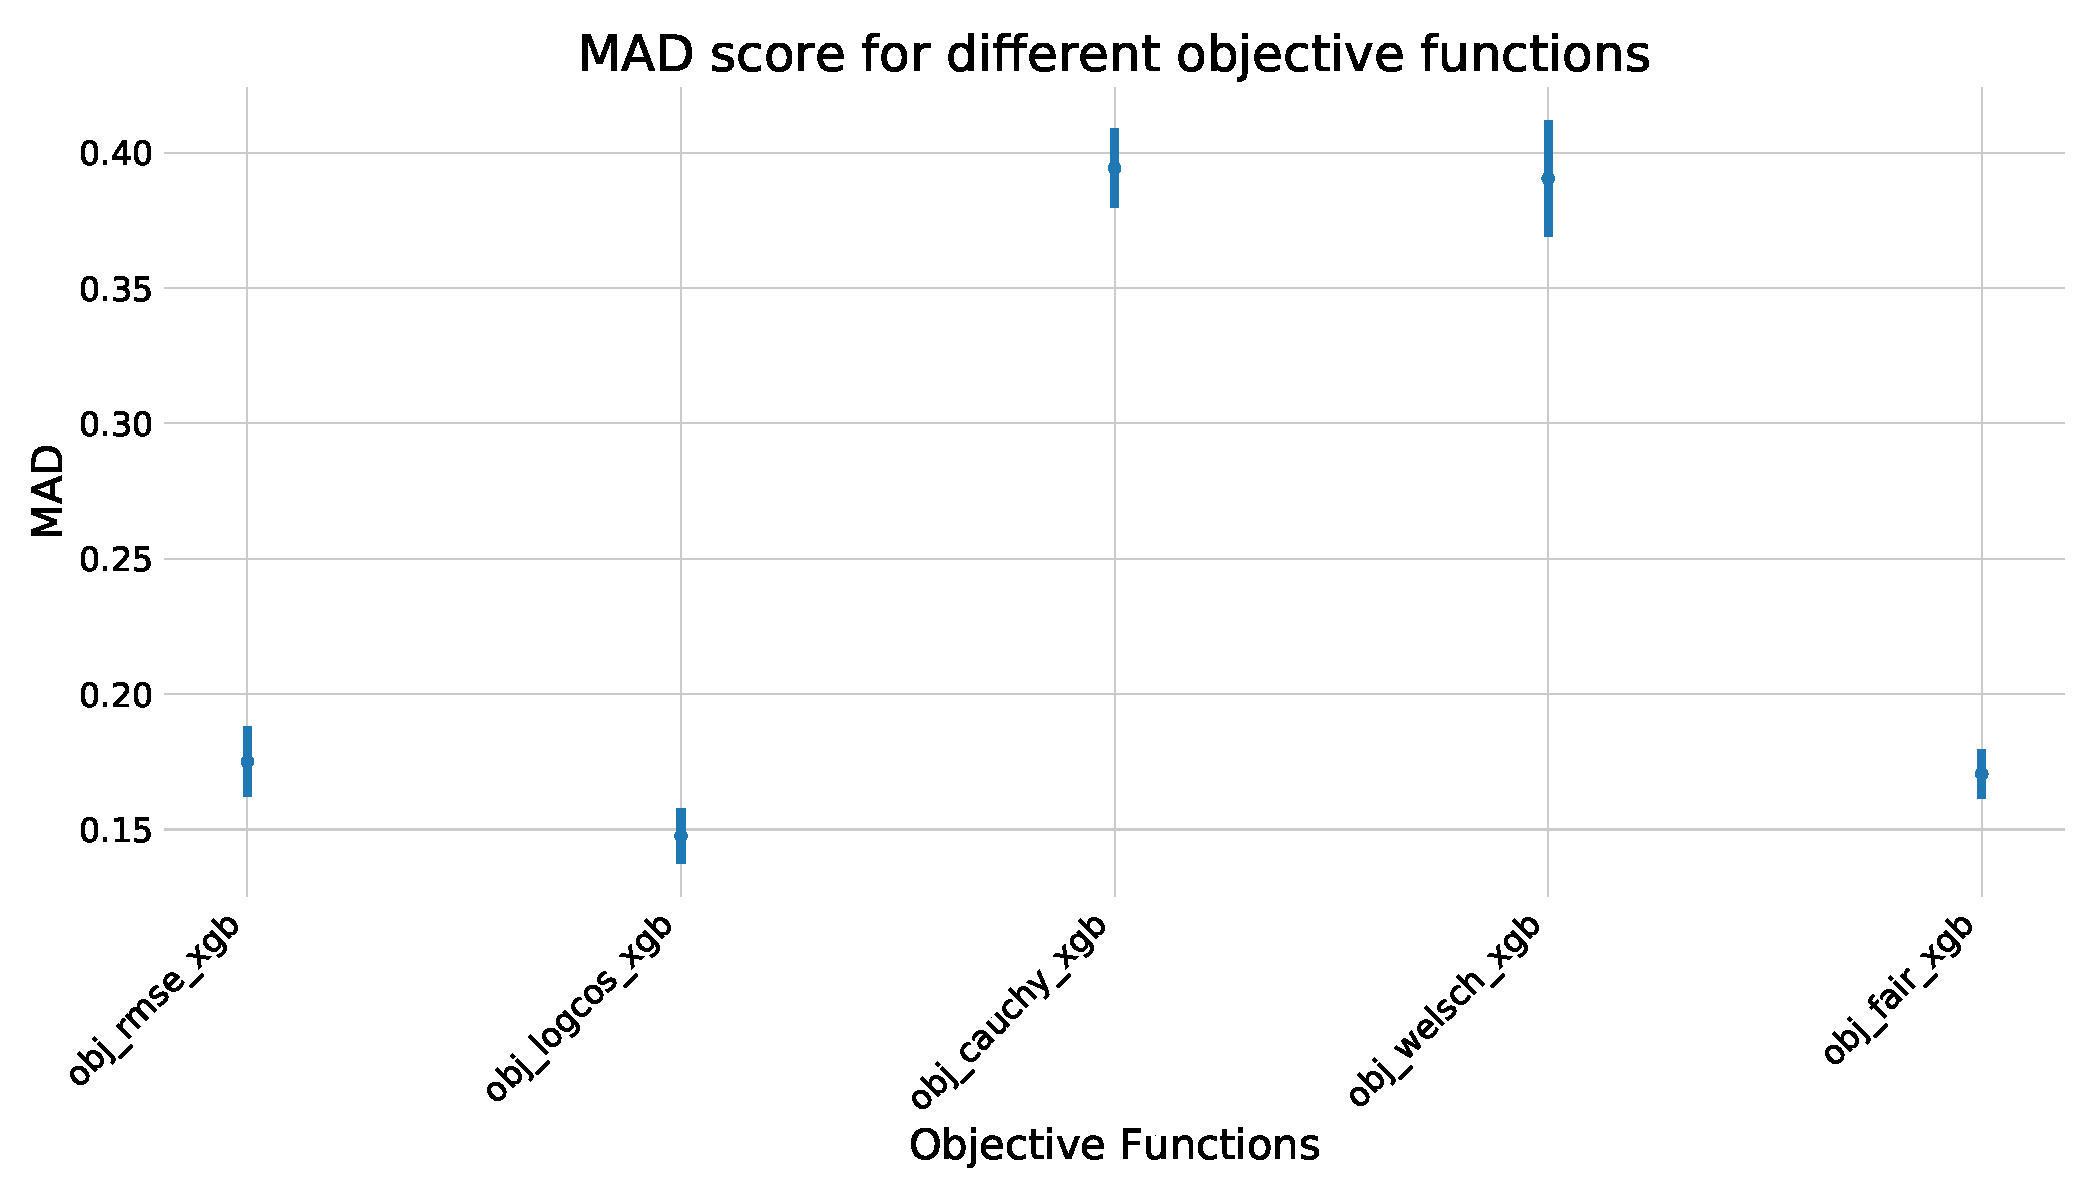
\includegraphics[width=0.9\textwidth, trim=0 35 0 40, clip]{figures/housing/Ejerlejlighed_v17_cut_all_Ncols_all__MAD_gridsearch_obj.pdf}
  \caption[Comparison of different objective functions][6pt]
          {Comparison of performance (measured using the median of the absolute deviation, MAD, for apartments) of the five different objective functions: RMSE, LogCosh, Cauchy, Welsch, and Fair. We see that the default objective function, RMSE, does a reasonable job, however, the LogCosh function is a clear improvement.
          } 
  \label{fig:h:objective_functions_performance}
\end{figure}



\begin{figure}
  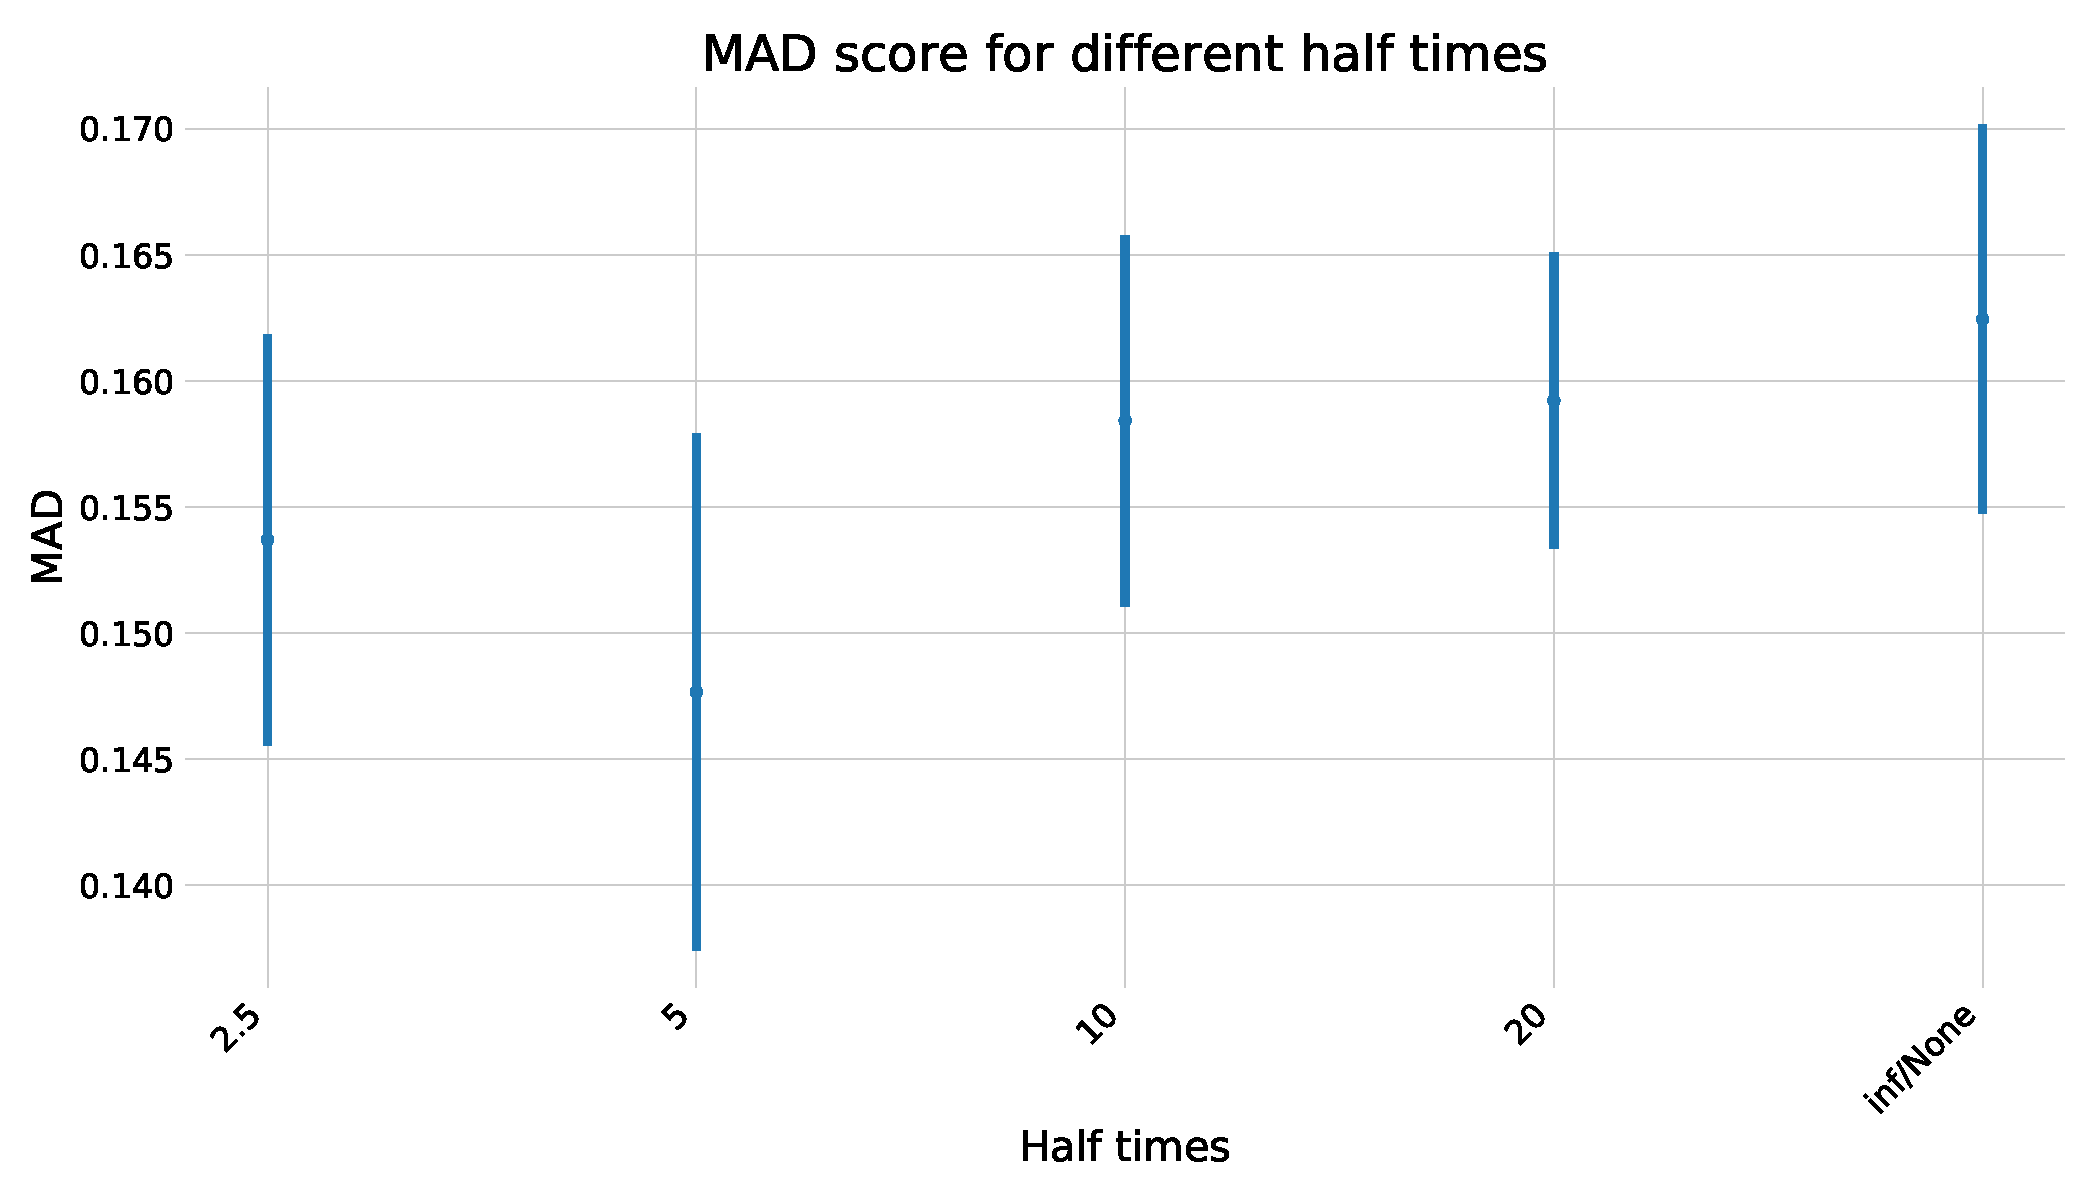
\includegraphics[width=0.9\textwidth, trim=0 0 0 40, clip]{figures/housing/Ejerlejlighed_v17_cut_all_Ncols_all__MAD_gridsearch_half.pdf}
  \caption[Comparison of different half times weights][6pt]
          {Comparison of performance (measured using the median of the absolute deviation, MAD, on apartments) of the five different half time weights: 2.5, 5, 10, 20, inf/None. We see that using no half time weights does has the worst performance, whereas a 5-year half time weight has the best performance (although with a very high uncertainty).
          } 
  \label{fig:h:half_time_performance}
\end{figure}



\begin{figure}
  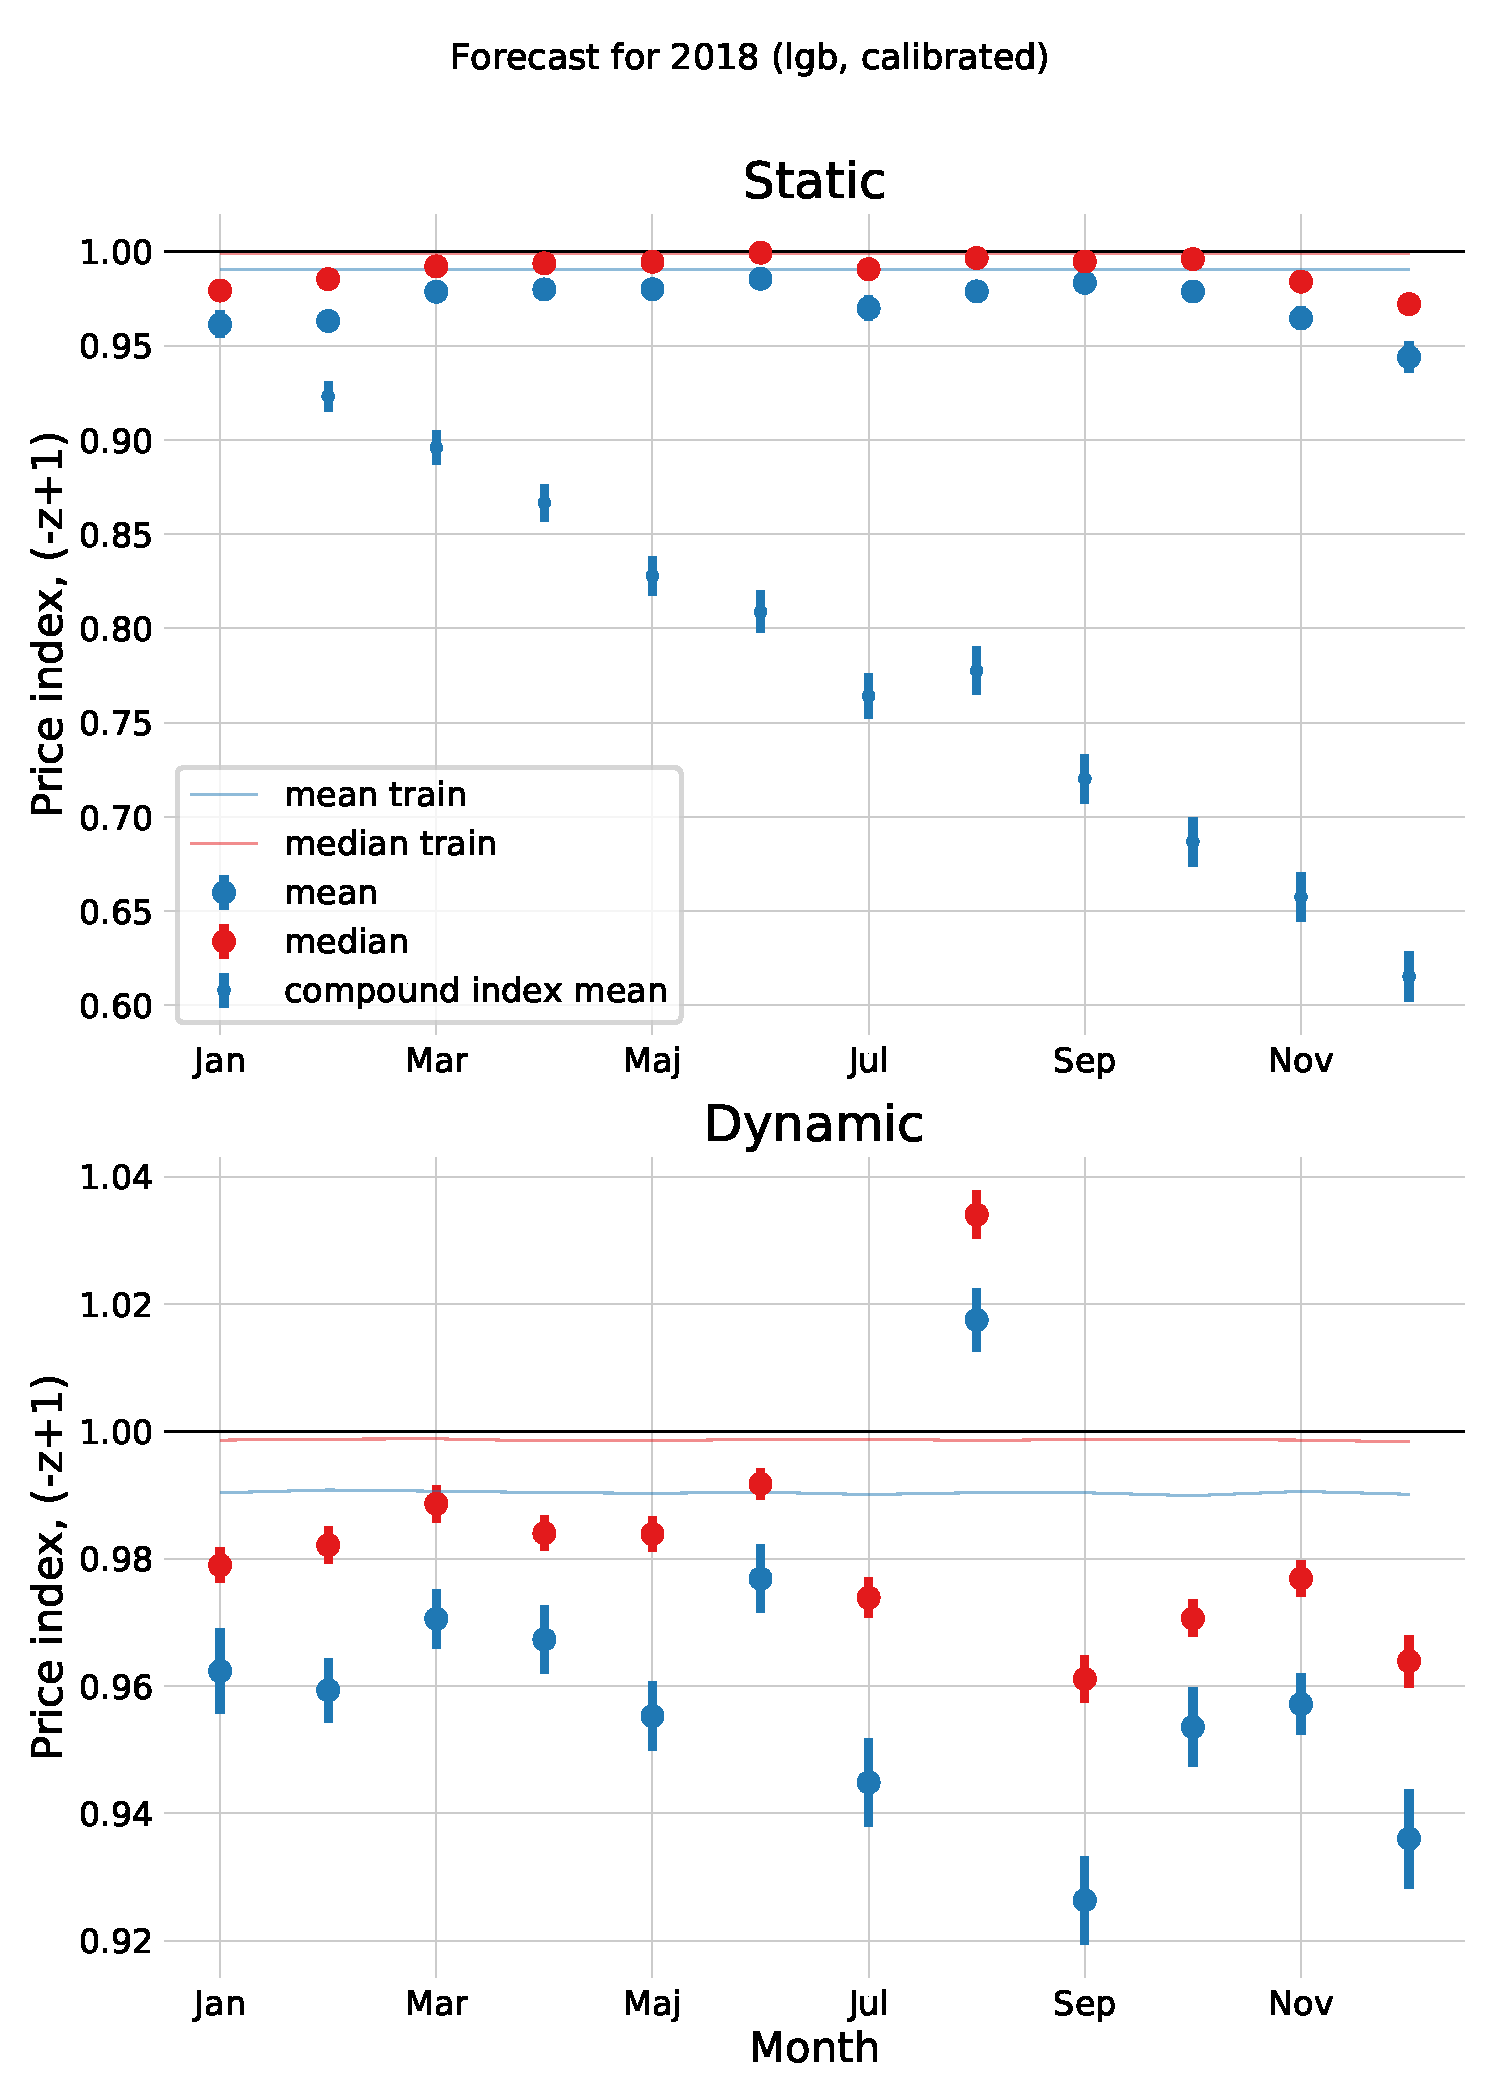
\includegraphics[width=0.9\textwidth, trim=0 0 0 70, clip]{figures/housing/Ejerlejlighed_v17_cut_all_Ncols_all__lgb_forecast_prediction_2018.pdf}
  \caption[2018 LGB Forecast][6pt]
          {Performance of 1-month forecasts for 2018 for apartments. For both plots the LGM model is trained on data up to (but excluding) 2018. Top) The performance of the static model's prediction on sales in the individual months of 2018 is shown for both the \textcolor{blue}{mean} and \textcolor{red}{median} of the $z$-scores. Bottom) Same as above, however this time based a dynamic model, i.e. a model which is retrained after every month to include the previous month's sales.
          } 
  \label{fig:h:forecast_2018_lgb}
\end{figure}









\section{Headings}\label{sec:headings1}\index{headings}

Tufte's books include the following heading levels: parts,
chapters,\sidenote{Parts and chapters are defined for the \texttt{tufte-book}
class only.}  sections, subsections, and paragraphs.  Not defined by default
are: sub-subsections and subparagraphs.

\begin{table}[h]
  \begin{center}
    \footnotesize%
    \begin{tabular}{lcr}
      \toprule
      Heading & Style & Size \\
      \midrule
      Part & roman & \measure{24}{36}{40} \\
      Chapter & italic & \measure{20}{30}{40} \\
      Section & italic & \measure{12}{16}{26} \\
      Subsection & italic & \measure{11}{15}{26} \\
      Paragraph & italic & 10/14 \\
      \bottomrule
    \end{tabular}
  \end{center}
  \caption{Heading styles used in \BE.}
  \label{tab:heading-styles}
\end{table}

\paragraph{Paragraph} Paragraph headings (as shown here) are introduced by
italicized text and separated from the main paragraph by a bit of space.

\chapter{Particle Physics and LEP}
\label{ch:particle_physcis_LEP}
% \immediate\write{./quote.sh \the\value{chapter}}
% \epigraph{\input{/tmp/fortune-\the\value{chapter}}}{--- \textup{\texttt{/usr/bin/fortune}}}

The \TL document classes define a style similar to the
style Edward Tufte uses in his books and handouts.  Tufte's style is known
for its extensive use of sidenotes, tight integration of graphics with
text, and well-set typography.  This document aims to be at once a
demonstration of the features of the \TL document classes
and a style guide to their use.

\section{Page Layout}\label{sec:page-layout}
\subsection{Headings}\label{sec:headings}\index{headings}
This style provides \textsc{a}- and \textsc{b}-heads (that is,
\Verb|\section| and \Verb|\subsection|), demonstrated above.

If you need more than two levels of section headings, you'll have to define
them yourself at the moment; there are no pre-defined styles for anything below
a \Verb|\subsection|.  As Bringhurst points out in \textit{The Elements of
Typographic Style}, 
% \cite{Bringhurst2005} 
you should ``use as many levels of
headings as you need: no more, and no fewer.''

The \TL classes will emit an error if you try to use
\linebreak\Verb|\subsubsection| and smaller headings.

% let's start a new thought -- a new section
\newthought{In his later books}, 
% \cite{Tufte2006}
 Tufte
starts each section with a bit of vertical space, a non-indented paragraph,
and sets the first few words of the sentence in \textsc{small caps}.  To
accomplish this using this style, use the \doccmddef{newthought} command:
\begin{docspec}
  \doccmd{newthought}\{In his later books\}, Tufte starts\ldots
\end{docspec}



\chapter{Quark Gluon Analysis}
\label{ch:quark_gluon_analysis}

\section{Sidenotes}\label{sec:sidenotes}
One of the most prominent and distinctive features of this style is the
extensive use of sidenotes.  There is a wide margin to provide ample room
for sidenotes and small figures.  Any \doccmd{footnote}s will automatically
be converted to sidenotes.\footnote{This is a sidenote that was entered
using the \texttt{\textbackslash footnote} command.}  If you'd like to place ancillary
information in the margin without the sidenote mark (the superscript
number), you can use the \doccmd{marginnote} command.\marginnote{This is a
margin note.  Notice that there isn't a number preceding the note, and
there is no number in the main text where this note was written.}





\begin{figure}
  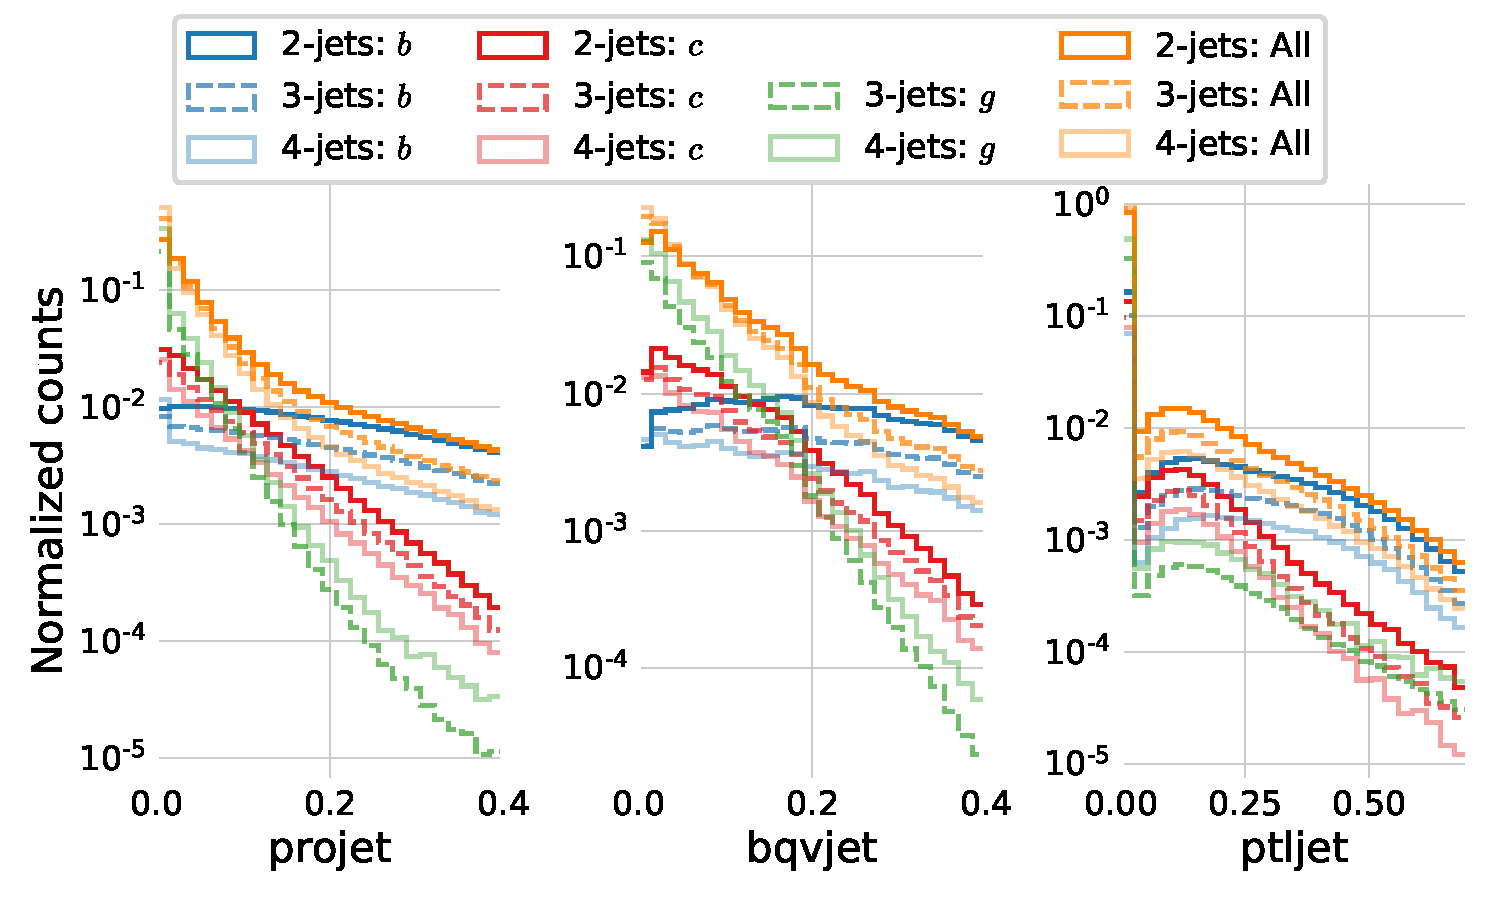
\includegraphics[width=0.95\textwidth, trim=0 0 0 0, clip]{figures/quarks/btagging_variables_hist-down_sample=1.00-ML_vars=vertex-selection=b-ejet_min=4-n_iter_RS_lgb=99-n_iter_RS_xgb=9-cdot_cut=0.90-version=19.pdf}
  \caption[Histograms of the vertex variables][6pt]
          {Histograms of the three vertex variables, \code{projet}, \code{bqvjet}, and \code{ptljet}, used as input variables in the b-tagging models. In blue colors the variables are shown for \textcolor{blue}{true b-jets}, in red for \textcolor{red}{true c-jets}, in green for \textcolor{green}{true g-jets}, and in orange for \textcolor{orange}{all of the jets} (including non q-matched). In fully opaque color are shown the distributions for 2-jet events, in dashed (and lighter color) 3-jet events, and in semi-transparent 4-jet events. Notice the logarithmic y-axis, that there are no g-jets for 2-jet events (as expected), and that all of the distributions are very similar not matter how many jets.
          } 
  \label{fig:q:vertex_variables}
\end{figure}



\begin{figure}
  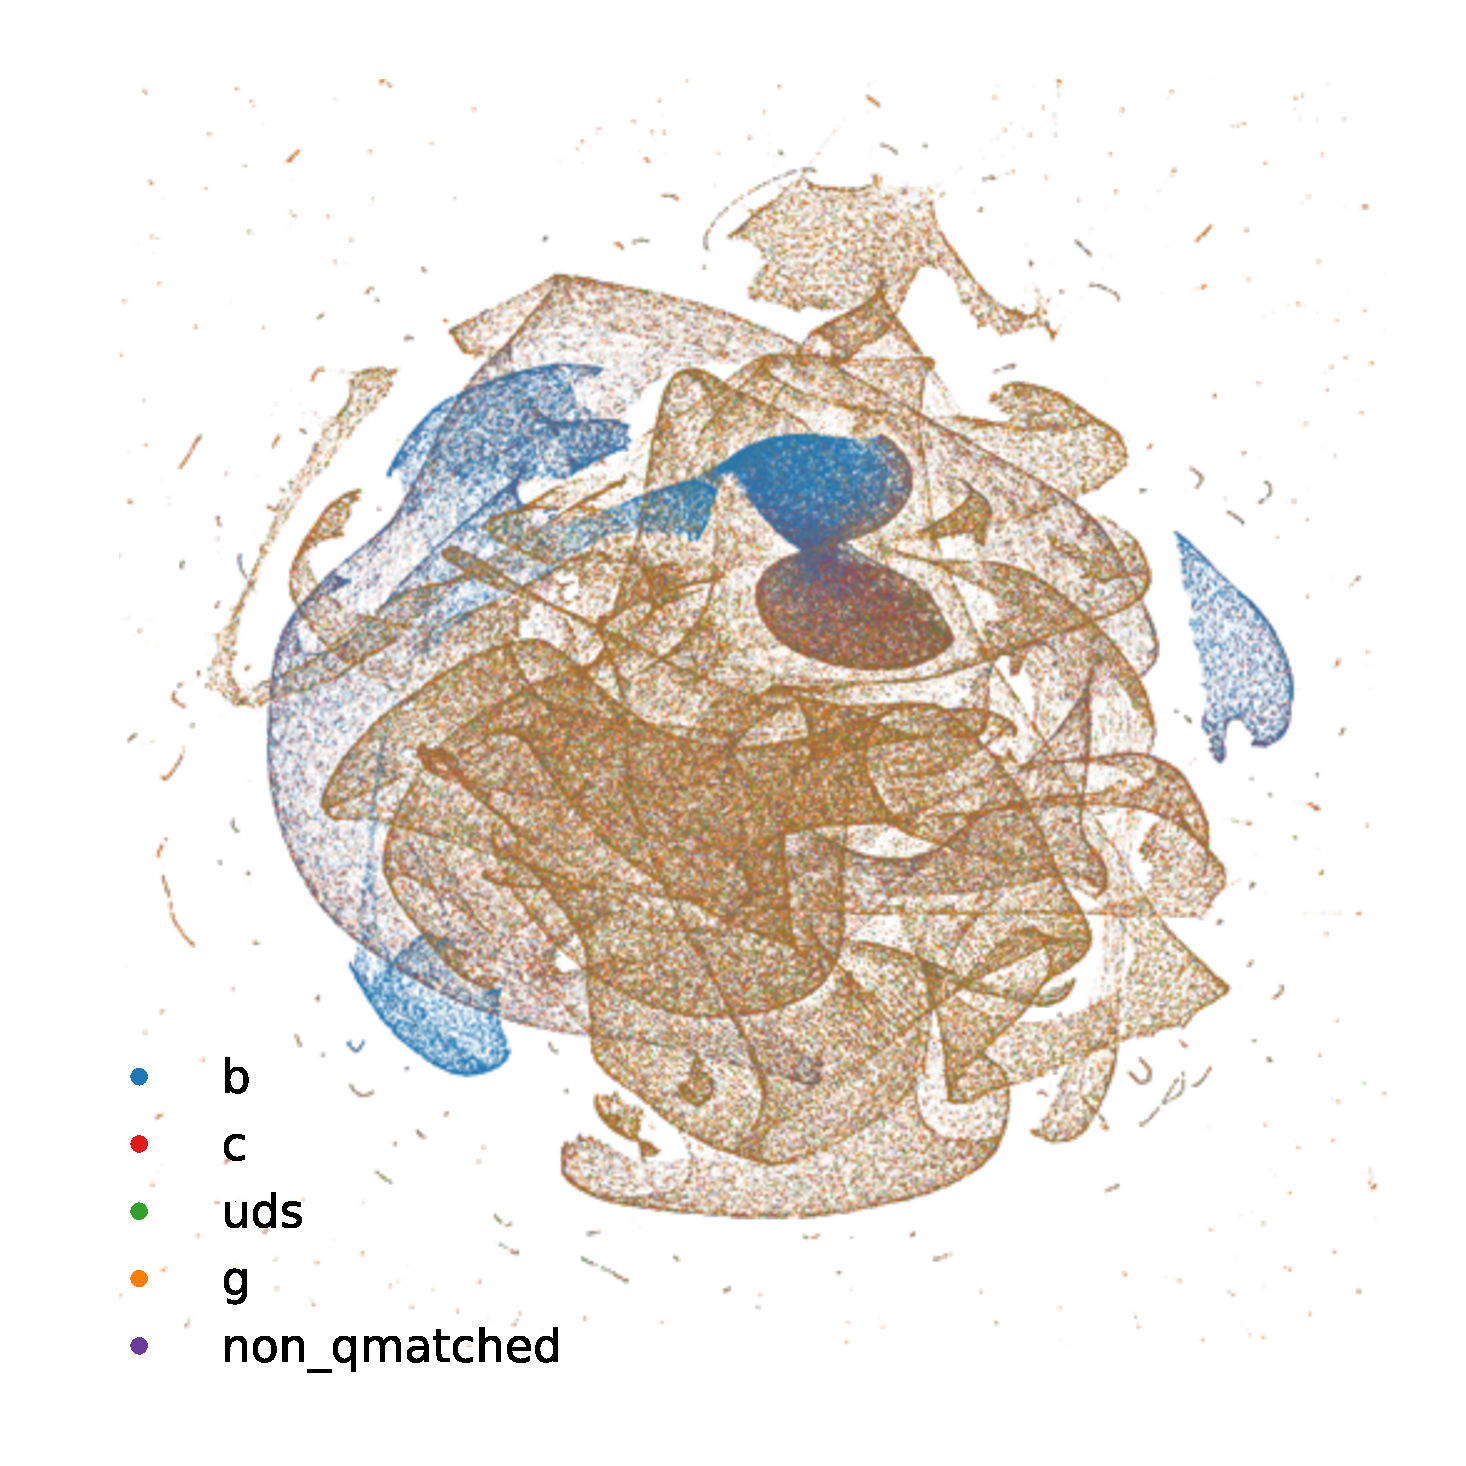
\includegraphics[width=0.95\textwidth, trim=20 20 50 50, clip]{figures/quarks/df_UMAP-X=1120952-n_neighbors=250-min_dist=0.2-metric=euclidean-input2b_njet=4_algorithm=UMAP_single.pdf}
  \caption[UMAP vizualisation of vertex variables][6pt]
          {Vizualisation of the vertex variables for the different categories: \textcolor{blue}{true b-jets} in blue, \textcolor{red}{true c-jets} in red, \textcolor{green}{true uds-jets} in green, \textcolor{orange}{true g-jets} in orange, and \textcolor{purple}{non q-matched}. The clustering is performed with the UMAP algorithm which outputs a 2D-projection. This projection is then visualized using the Datashader which takes takes care of point size, avoids over- and under-plotting, and color intensity. 
          } 
  \label{fig:q:UMAP_vertex}
\end{figure}



\begin{figure}
  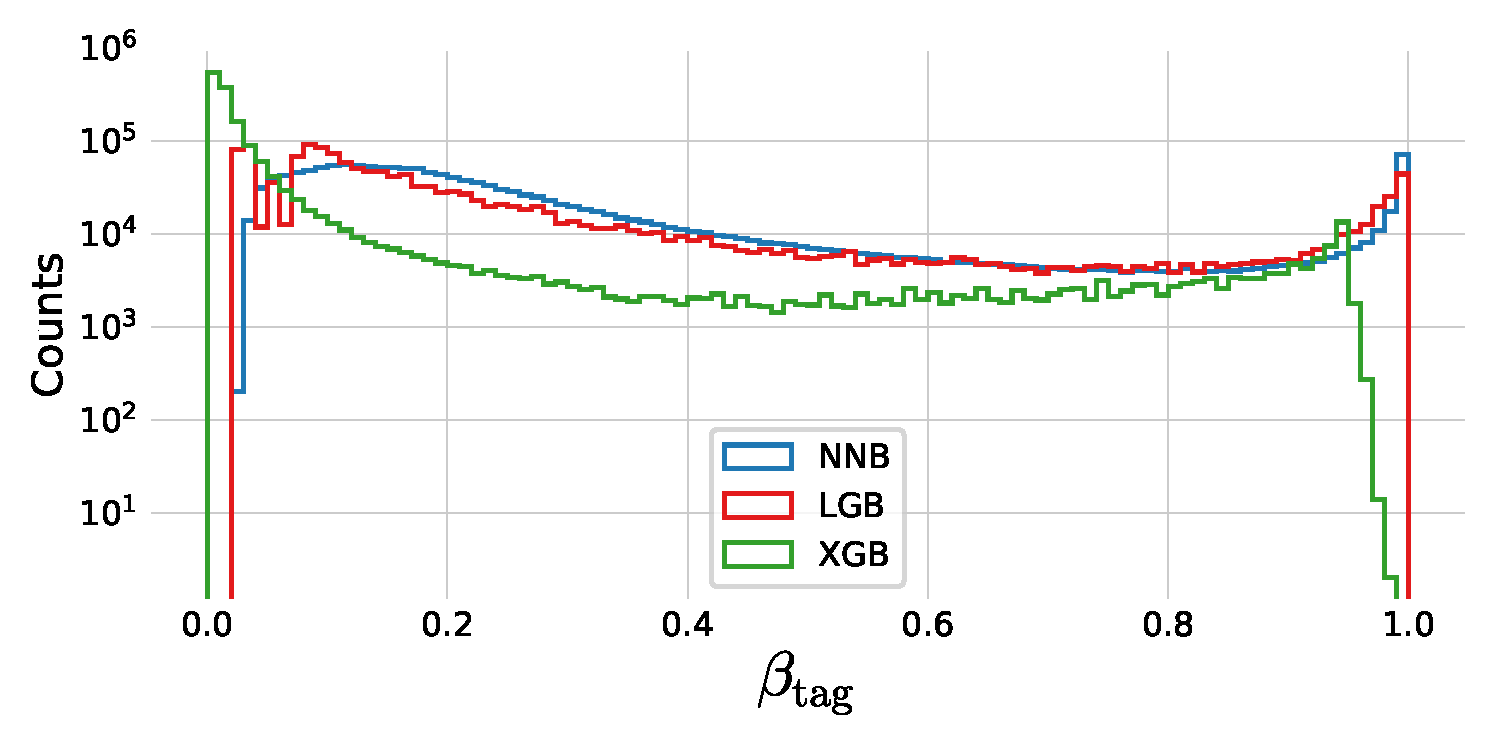
\includegraphics[width=0.95\textwidth, trim=0 0 0 30, clip]{figures/quarks/y_pred_3_jet_hist-down_sample=1.00-ML_vars=vertex-selection=b-ejet_min=4-n_iter_RS_lgb=99-n_iter_RS_xgb=9-cdot_cut=0.90-version=19.pdf}
  \caption[b-tag scores in 3-jet events][6pt]
          {Histogram of b-tag scores (model prediction) in 3-jet events for \textcolor{blue}{NNB} (the neural network trained by ATLAS, also called \code{nnbjet}) in blue, \textcolor{red}{LGB} in red, and \textcolor{green}{XGB} in green. We see that the LGB predictions closely match those of NNB which is a good confirmation of a successful fit.  
          } 
  \label{fig:q:btag_scores_3j}
\end{figure}




\begin{figure}
  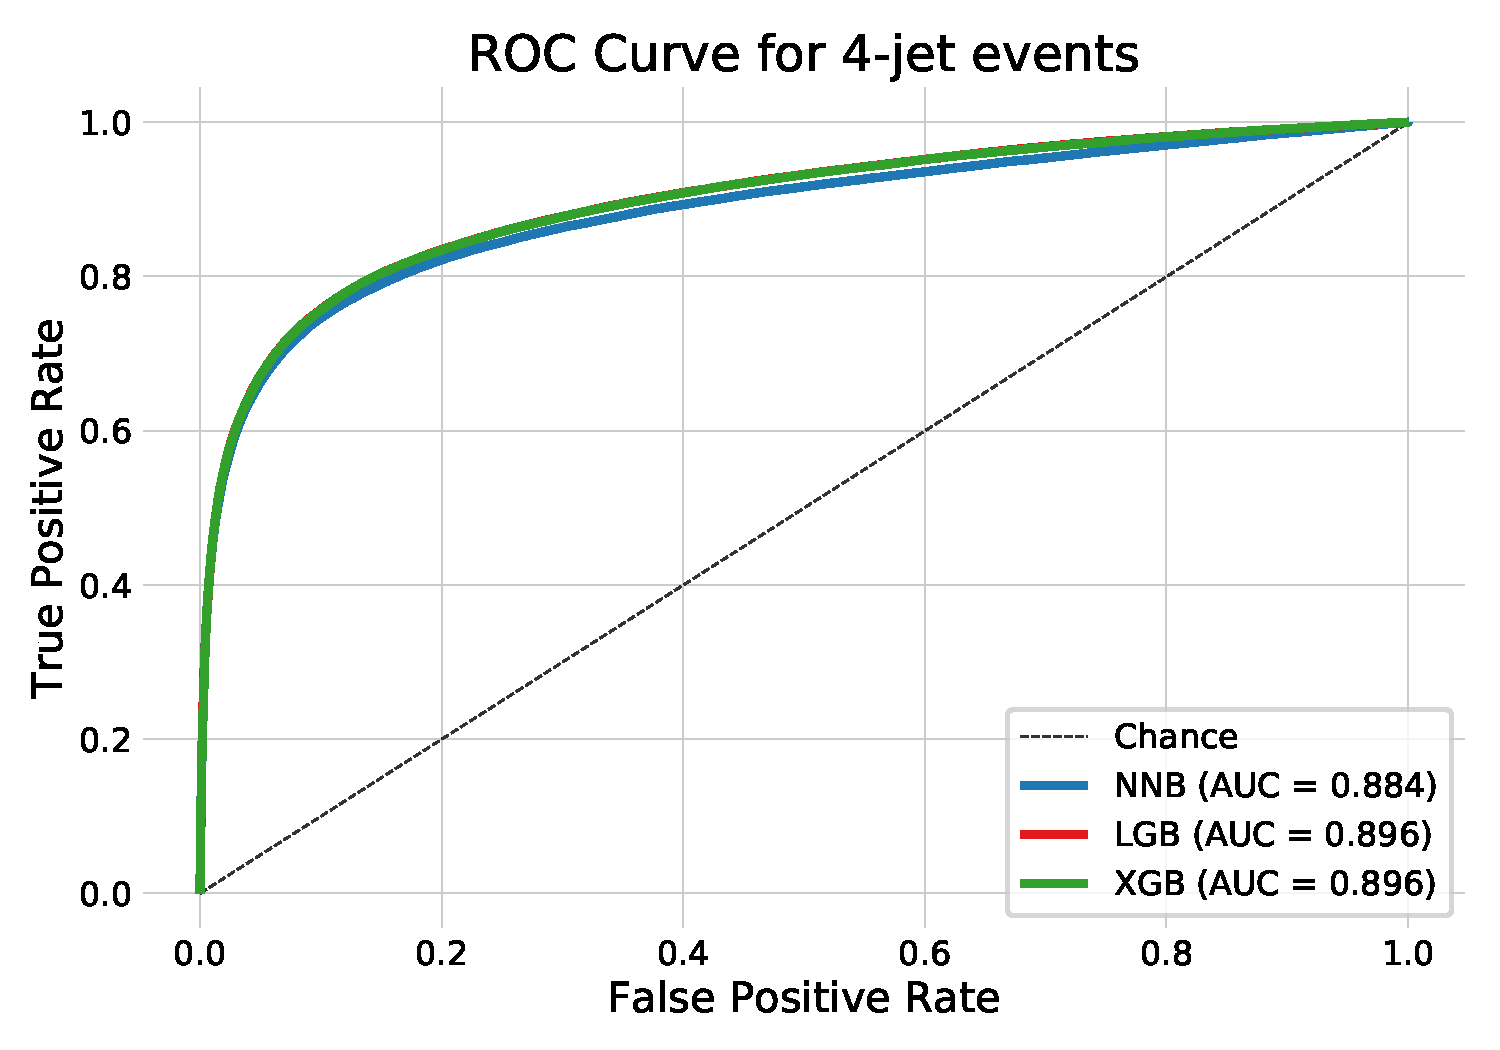
\includegraphics[width=0.95\textwidth, trim=10 10 10 40, clip]{figures/quarks/ROC_4_jet-down_sample=1.00-ML_vars=vertex-selection=b-ejet_min=4-n_iter_RS_lgb=99-n_iter_RS_xgb=9-cdot_cut=0.90-version=19.pdf}
  \caption[ROC curve for b-tag in 4-jet events][6pt]
          {ROC curve of the three b-tag models in 3-jet events for \textcolor{blue}{NNB} (the neural network trained by ATLAS, also called \code{nnbjet}) in blue, \textcolor{red}{LGB} in red, and \textcolor{green}{XGB} in green. In the legend the Area Under Curve (AUC) is also shown. Notice that the LGB and XGB models share performance and it is thus due to overplotting that only the green line for XGB can be seen. In the particle physics community False Positive Rate (FPR) is sometimes better known as background efficiency and True Positive Rate (TPR) as signal efficiency.  
          } 
  \label{fig:q:roc_btag_4j}
\end{figure}




\begin{figure}
  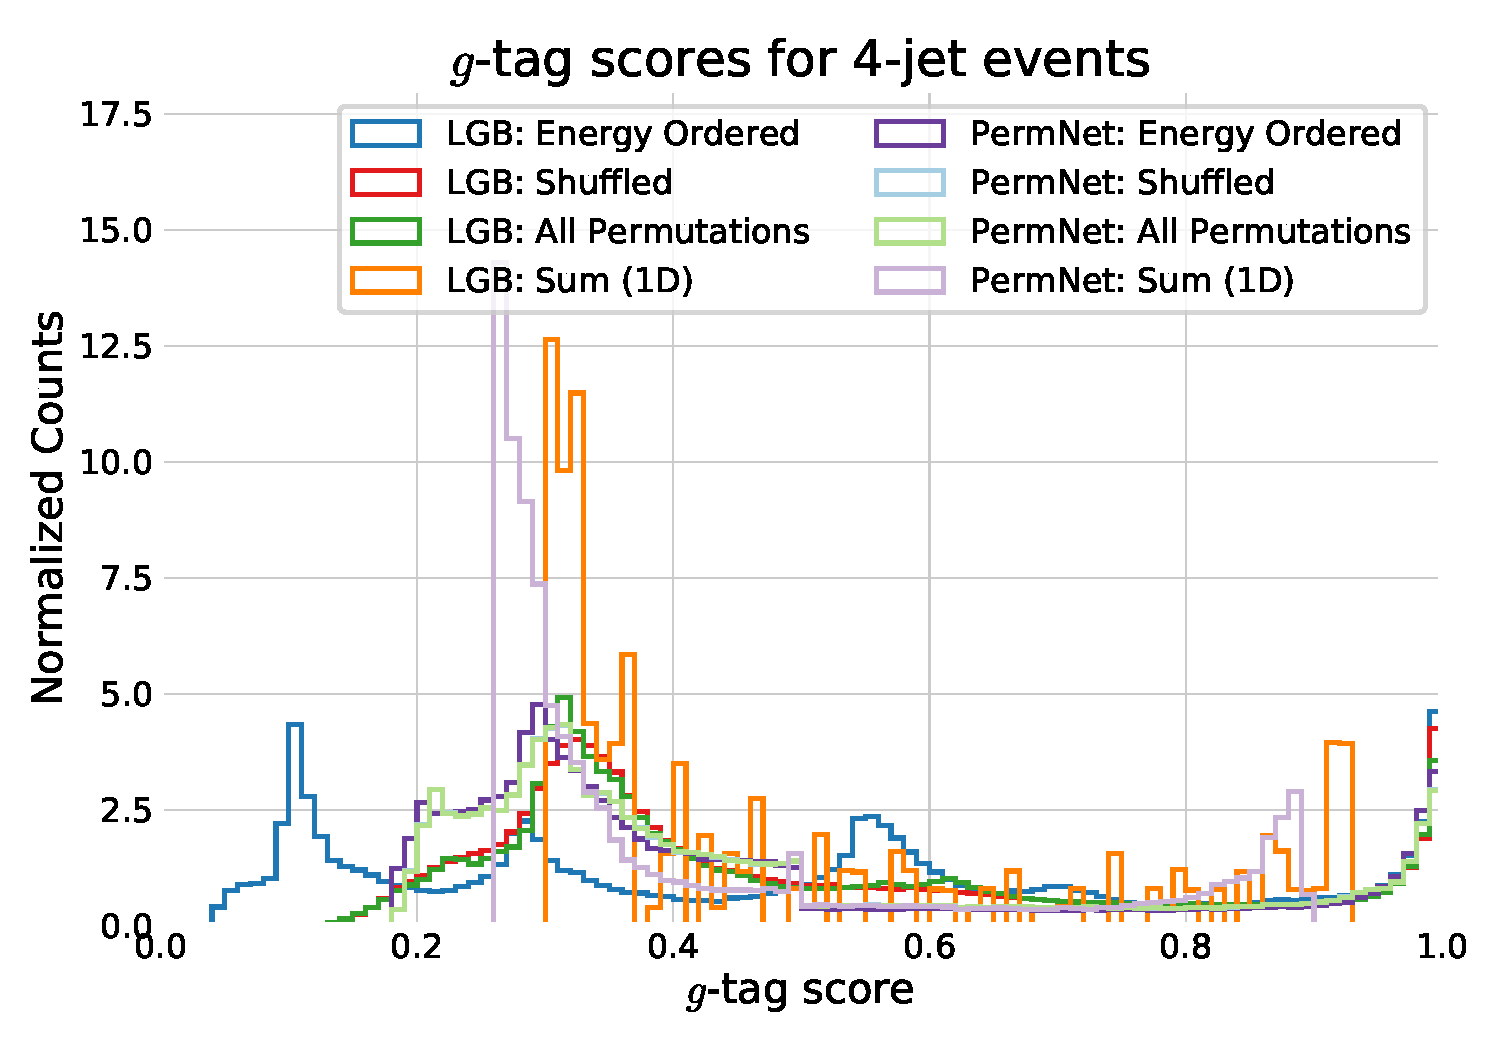
\includegraphics[width=0.95\textwidth, trim=10 10 10 40, clip]{figures/quarks/gtag_y_pred_4_jet_hist-down_sample=1.00-ML_vars=vertex-selection=b-ejet_min=4-n_iter_RS_lgb=99-n_iter_RS_xgb=9-cdot_cut=0.90-version=19.pdf}
  \caption[g-tag scores in 4-jet events][6pt]
          {
            Histogram of g-tag scores (model prediction) in 4-jet events for \textcolor{blue}{LGB: Energy Ordered} in blue, \textcolor{red}{LGB: Shuffled} in red, \textcolor{green}{LGB: All Permutations} in green, \textcolor{orange}{LGB: Sum 1D} in orange, \textcolor{purple}{PermNet: Energy Ordered} in purple, \textcolor{light-blue}{PermNet: Shuffled} in light-blue, \textcolor{light-green}{PermNet: All Permutations} in light-green, \textcolor{light-purple}{PermNet: Sum 1D} in light-purple.  Here LGB and PermNet are the two different type of models and \q{Energy Ordered}, \q{Shuffled}, \q{All Permutations}, and \q{Sum 1D} are the different methods used for making the input data permutation invariant.  
          }   
  \label{fig:q:gtag_scores_4j}
\end{figure}


\begin{figure}
  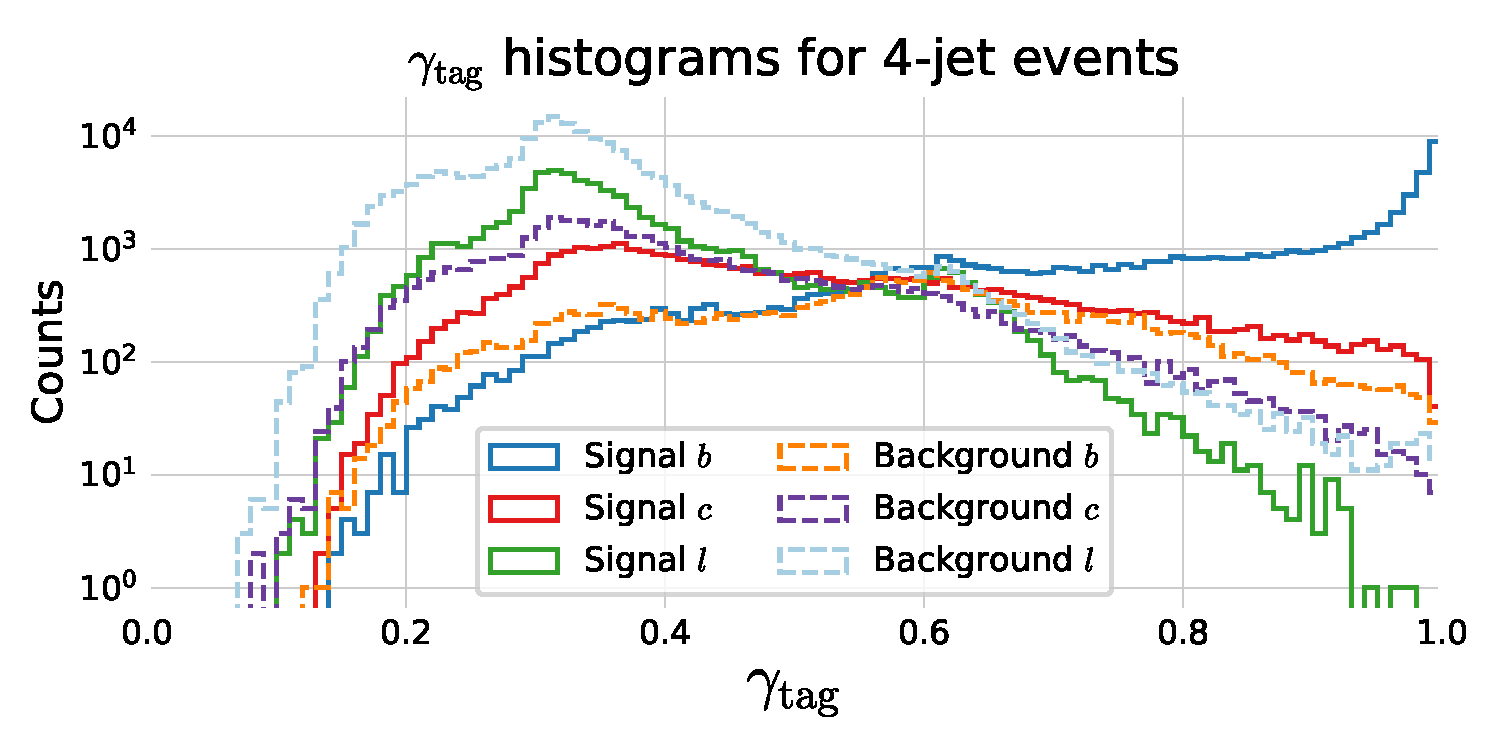
\includegraphics[width=0.95\textwidth, trim=10 10 10 40, clip]{figures/quarks/gtag-histogram-sigbkg-down_sample=1.00-ML_vars=vertex-selection=b-ejet_min=4-n_iter_RS_lgb=99-n_iter_RS_xgb=9-cdot_cut=0.90-version=19-njet=4.pdf}
  \caption[g-tag scores in 4-jet events for signal and background][6pt]
          {Histogram of g-tag scores (model prediction) from the LGB-model in 4-jet events for \textcolor{blue}{b signal} in blue, \textcolor{red}{c signal} in red, \textcolor{green}{l signal} in green, \textcolor{orange}{b background} in orange, \textcolor{purple}{c background} in purple, \textcolor{light-blue}{l background} in light-blue.
          } 
  \label{fig:q:gtag_scores_4j_sig_bkg}
\end{figure}





\begin{figure}
  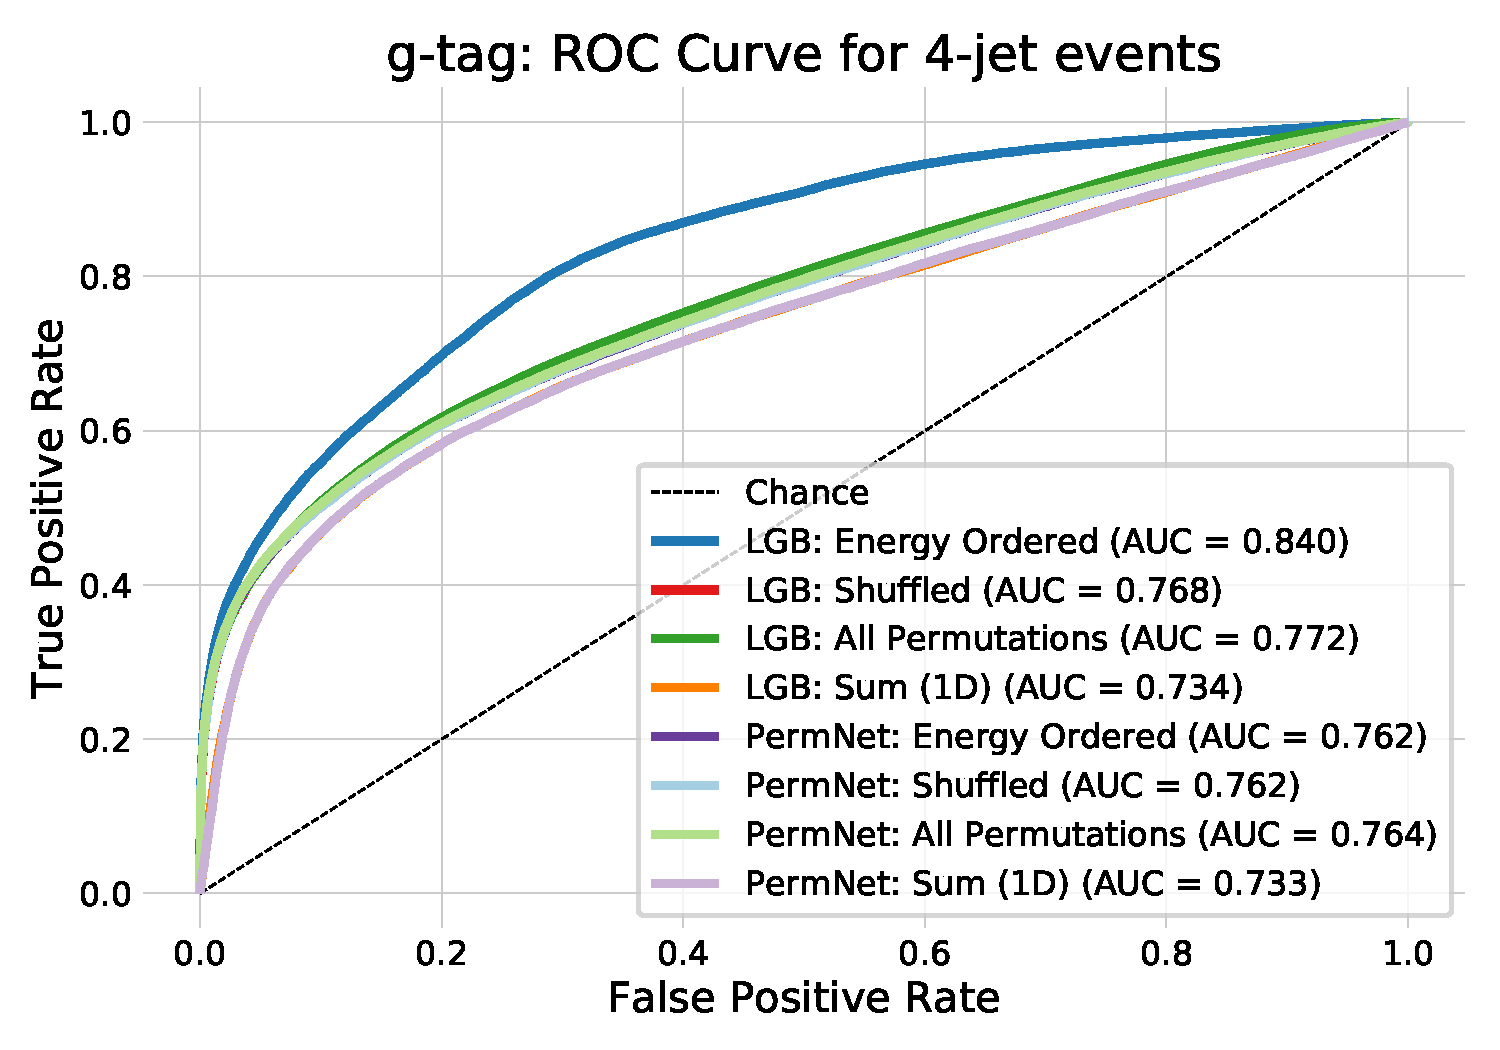
\includegraphics[width=0.95\textwidth, trim=10 10 10 40, clip]{figures/quarks/gtag_ROC_4_jet-down_sample=1.00-ML_vars=vertex-selection=b-ejet_min=4-n_iter_RS_lgb=99-n_iter_RS_xgb=9-cdot_cut=0.90-version=19.pdf}
  \caption[ROC curve for g-tag in 4-jet events][6pt]
          {ROC curve of the eight g-tag models in 4-jet events. First one in dashed black is the ROC curve that you get by random chance. The colors are the same as in \figref{fig:q:gtag_scores_4j} and in the legend also the Area Under the ROC curve (AUC) is shown. 
          Notice that the LGB model which uses the energy ordered data produced the best model, however, this model is not permutation invariant. Of the permutation invariant models (the rest), the LGB model trained on all permutations of the b-tags performs highest. The lowest performing models are the two models trained only on the 1-dimensional sum of b-tags, as expected, however, still with a better performance than expected by the author.  
          } 
  \label{fig:q:roc_gtag_4j}
\end{figure}





\begin{figure}
  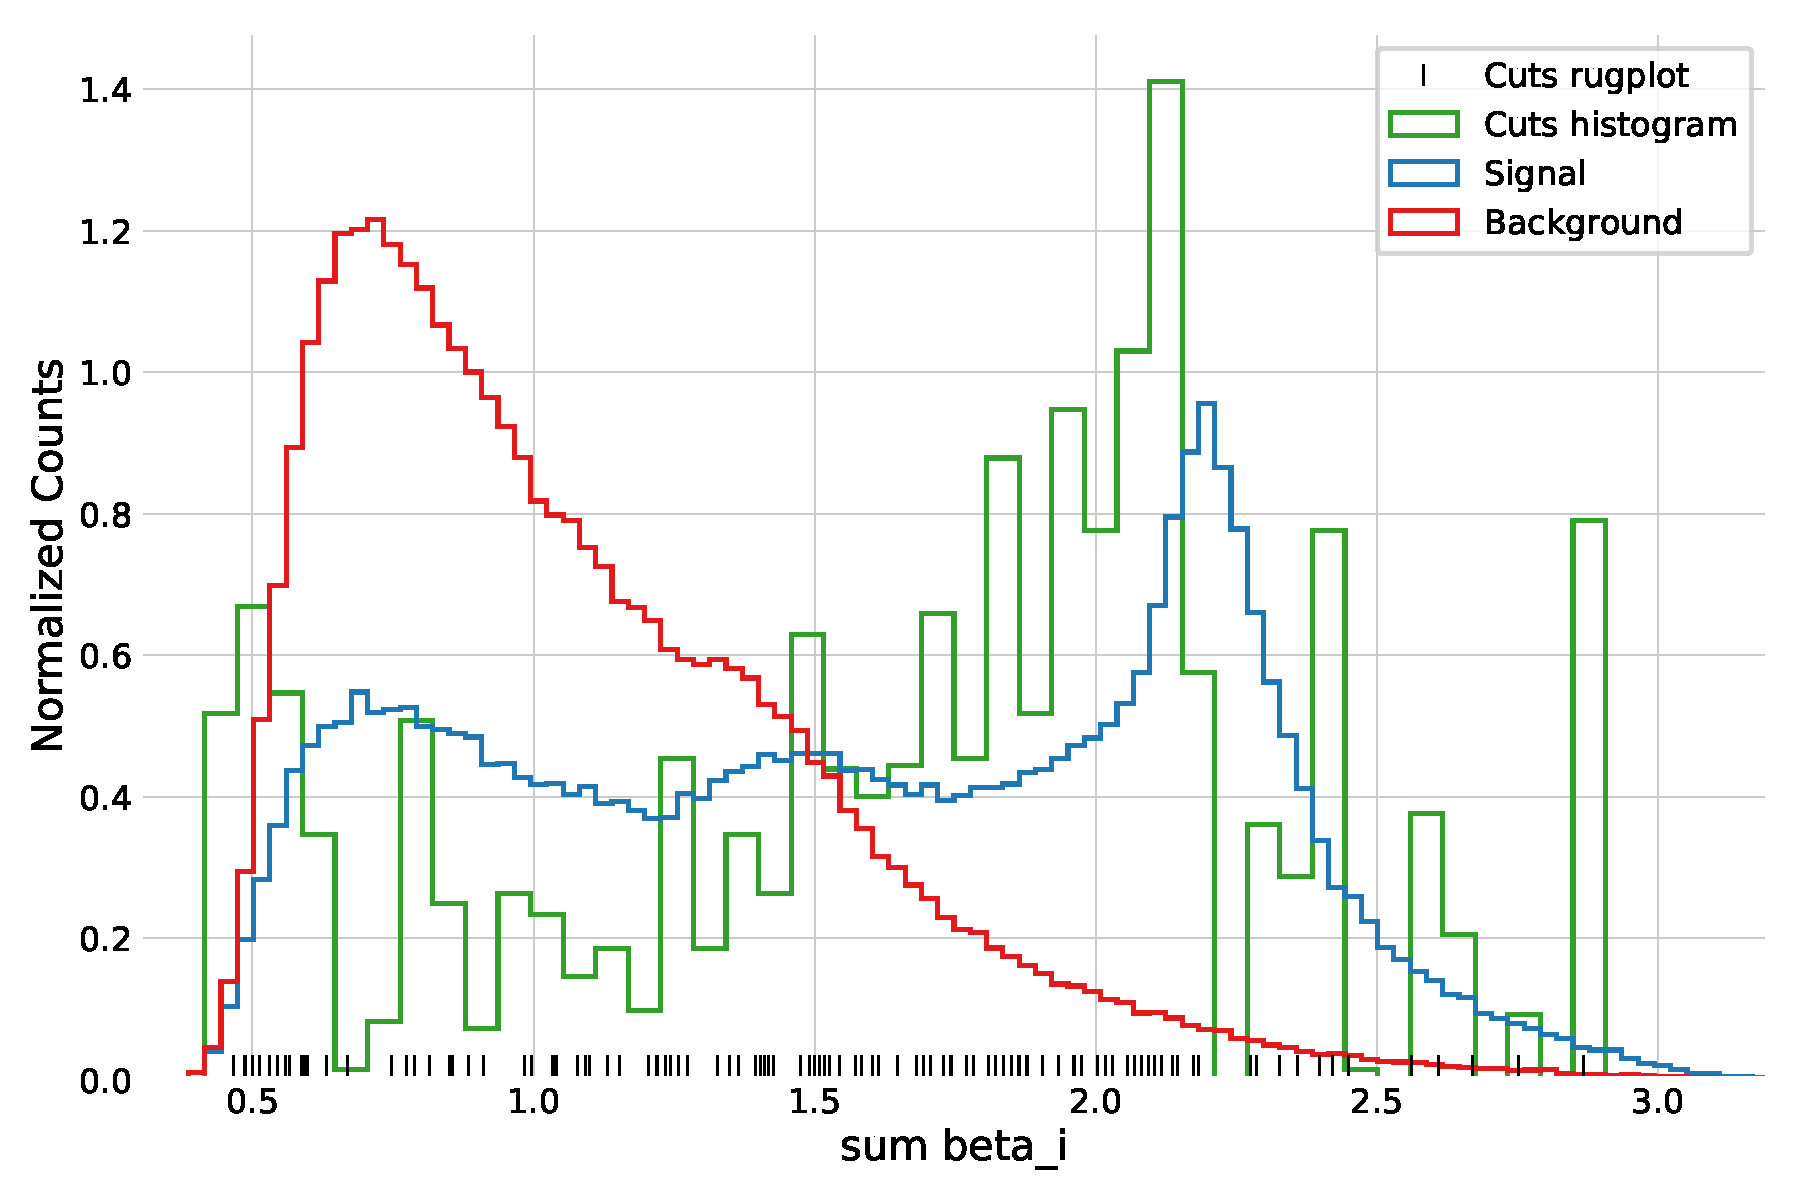
\includegraphics[width=0.95\textwidth, trim=10 10 10 20, clip]{figures/quarks/gtag_sum_method_njet=4-down_sample=1.00-ML_vars=vertex-selection=b-ejet_min=4-n_iter_RS_lgb=99-n_iter_RS_xgb=9-cdot_cut=0.90-version=19.pdf}
  \caption[1D Sum Model Cuts for 4-jets][6pt]
          {Histogram of the distribution of \textcolor{blue}{signal} in blue and \textcolor{red}{background} in red for 1-dimensional sum of b-tags training data. A histogram of the \textcolor{green}{cut values} from the LGB model trained on this data is shown in green together with a rug plot of the cut values in black. Notice how most of the cuts match up with the signal peak at around a $\sum \beta_i \sim 2.1$, however, there are also quite a lot of cuts around $\sum \beta_i \sim 0.5$.
          } 
  \label{fig:q:1d_sum_model_cuts_4j}
\end{figure}


\begin{figure}
  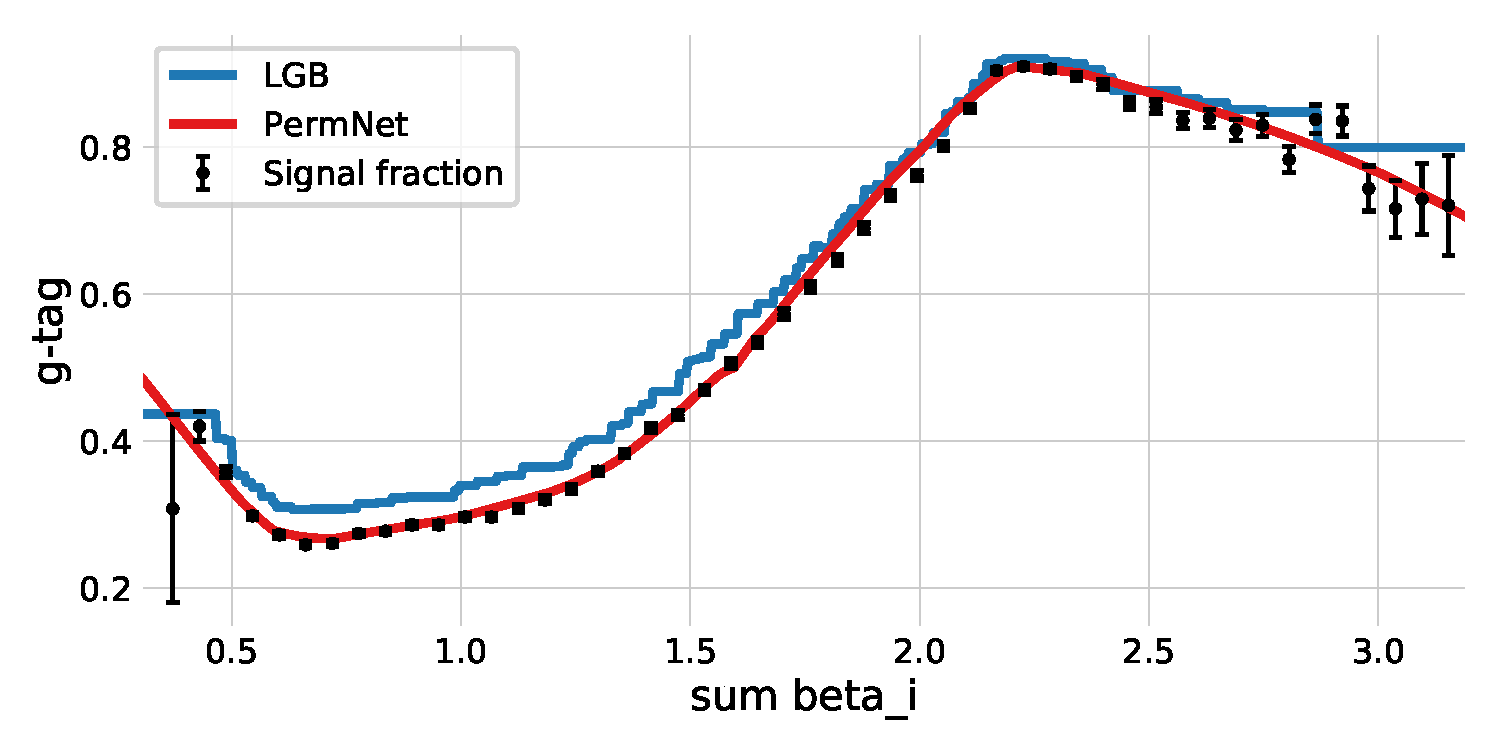
\includegraphics[width=0.95\textwidth, trim=10 10 10 20, clip]{figures/quarks/gtag_sum_models_njet=4-down_sample=1.00-ML_vars=vertex-selection=b-ejet_min=4-n_iter_RS_lgb=99-n_iter_RS_xgb=9-cdot_cut=0.90-version=19.pdf}
  \caption[1D Sum Models Predictions and Signal Fraction for 4-jets][6pt]
          {Plot of the (1D) g-tag scores as a function of $\sum \beta_i$ for the \textcolor{blue}{LGB} model in blue and the \textcolor{red}{PermNet} model in red. Here the g-tag scores are just the models' output values when input a uniformly spaced grid of $\sum \beta_i$ values between 0 and 4. The signal fraction (based on the signal and background histograms in \figref{fig:q:1d_sum_model_cuts_4j}) is plotted as black error bars where the size of the error bars is based on the propagated uncertainties of the signal and background histogram assuming Poissonian statistics. Notice how both models capture the overall trend of the signal fraction with the PermNet being particularly close. 
          } 
  \label{fig:q:1d_sum_models_signal_fraction_4j}
\end{figure}




\begin{figure}
  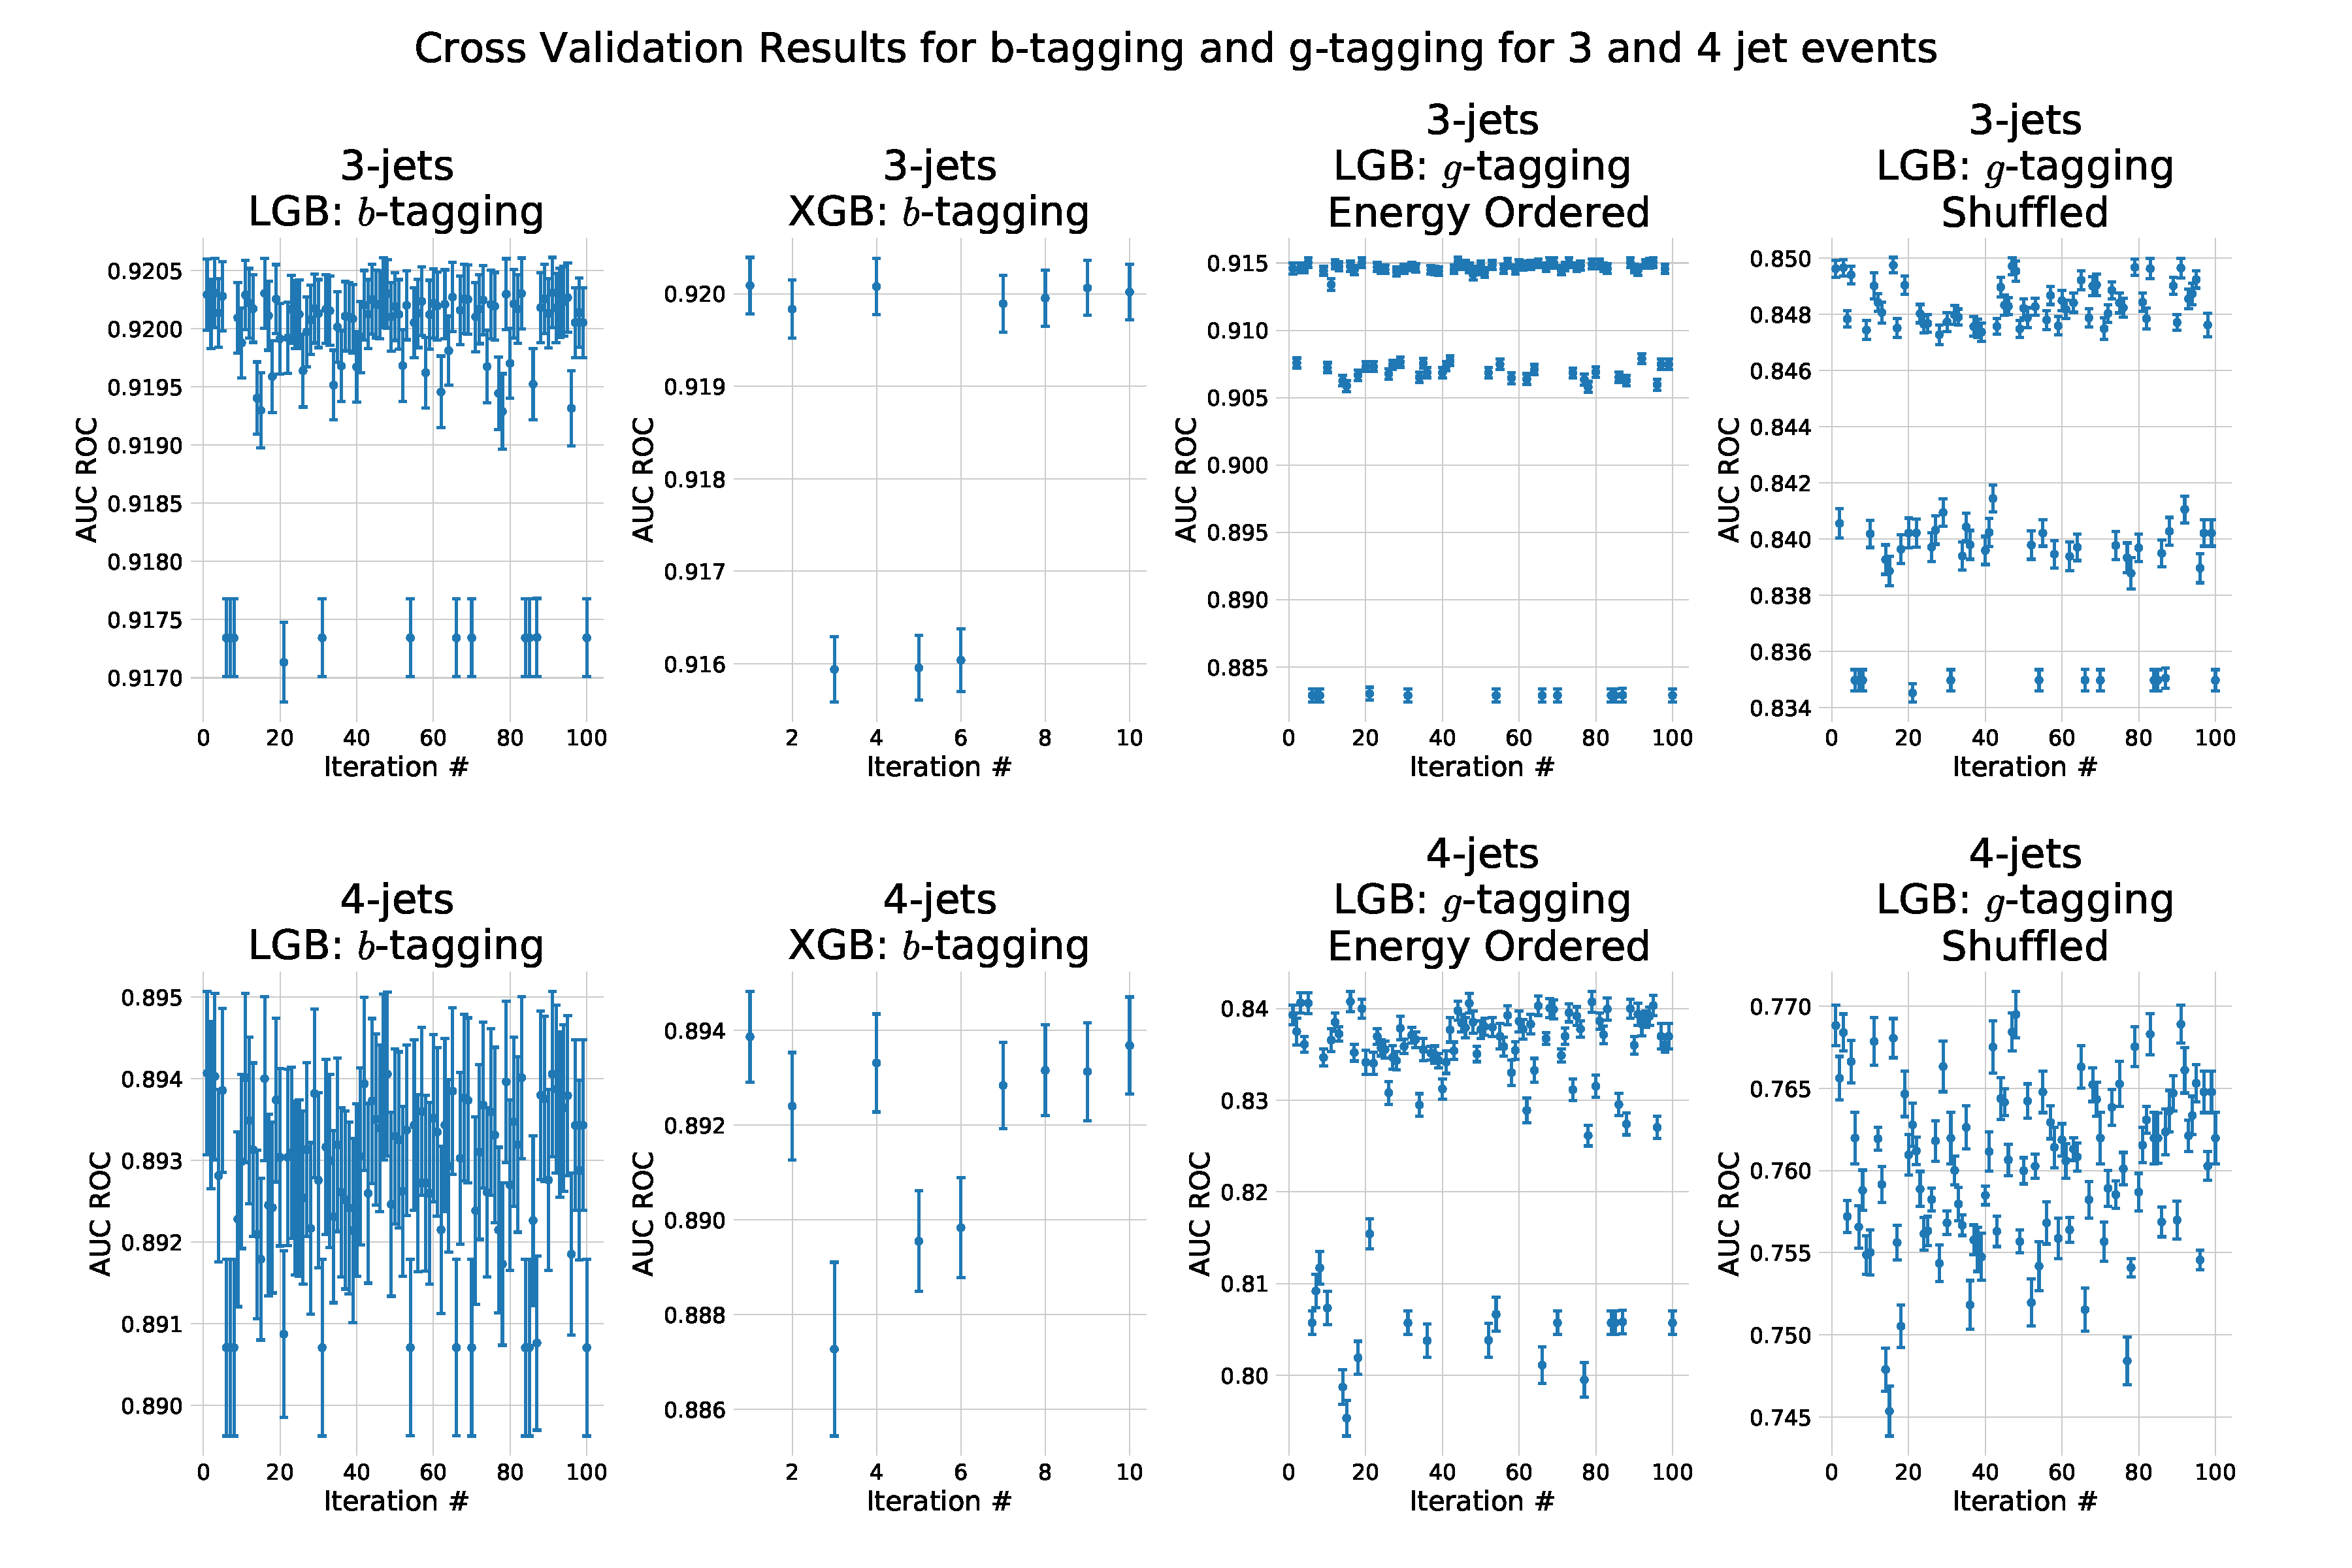
\includegraphics[width=0.95\textwidth, trim=10 10 10 60, clip]{figures/quarks/cv_res_lgb-down_sample=1.00-ML_vars=vertex-selection=b-ejet_min=4-n_iter_RS_lgb=99-n_iter_RS_xgb=9-cdot_cut=0.90-version=19.pdf}
  \caption[Hyperparameter Optimization of b- and g-tagging][6pt]
          {Hyperparameter Optimization (HPO) results after running 100 iterations of Random Search (only 10 for XGB). In the top row are the results of the 3-jet models and in the bottom row the results of the 4-jet models. From left to right, we have first) the b-tagging results of LGB, second) the b-tagging results of XGB using only 10 iterations of RS, third) the g-tagging results of LGB fit on the Energy Ordered b-tags, and forth) the g-tagging results of LGB fit on the shuffled b-tags. Notice the different ranges on the y-axes.
          } 
  \label{fig:q:CV_res_iterations}
\end{figure}


\begin{figure}
  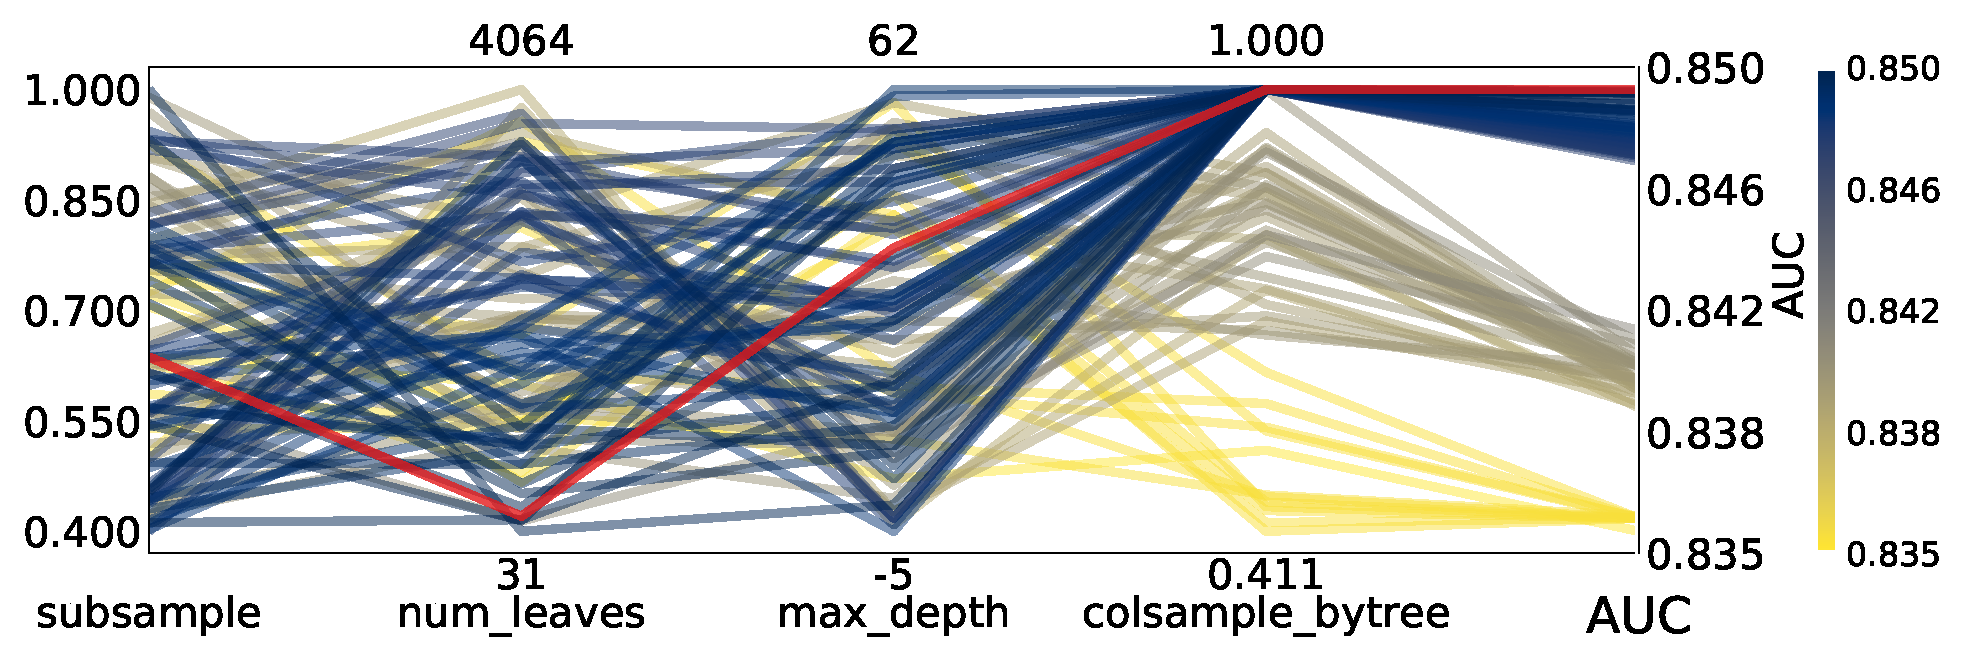
\includegraphics[width=0.95\textwidth, trim=0 0 0 0, clip]{figures/quarks/CV_viz-njet=3-name=lf_gtag_shuffled_lgb_down_sample=1.00-ML_vars=vertex-selection=b-ejet_min=4-n_iter_RS_lgb=99-n_iter_RS_xgb=9-cdot_cut=0.90-version=19.pdf}
  \caption[Overview of Hyperparamaters of g-tagging for 3-jet shuffled events][6pt]
          {Hyperparameter optimization results of g-tagging for 3-jet shuffled events. The results are shown as parallel coordinates with each hyperparameter along the x-axis and the value of that parameter on the y-axis. Each line is an event in the 4-dimensional space colored according to the performance of that hyperparameter as measured by AUC from \textcolor{viridis-dark}{highest} AUC in dark blue to \textcolor{viridis-light}{lowest} AUC in yellow. The \textcolor{red}{single best hyperparameter} is shown in red. 
          } 
  \label{fig:q:CV_res_parallel_coords}
\end{figure}



\begin{figure}
  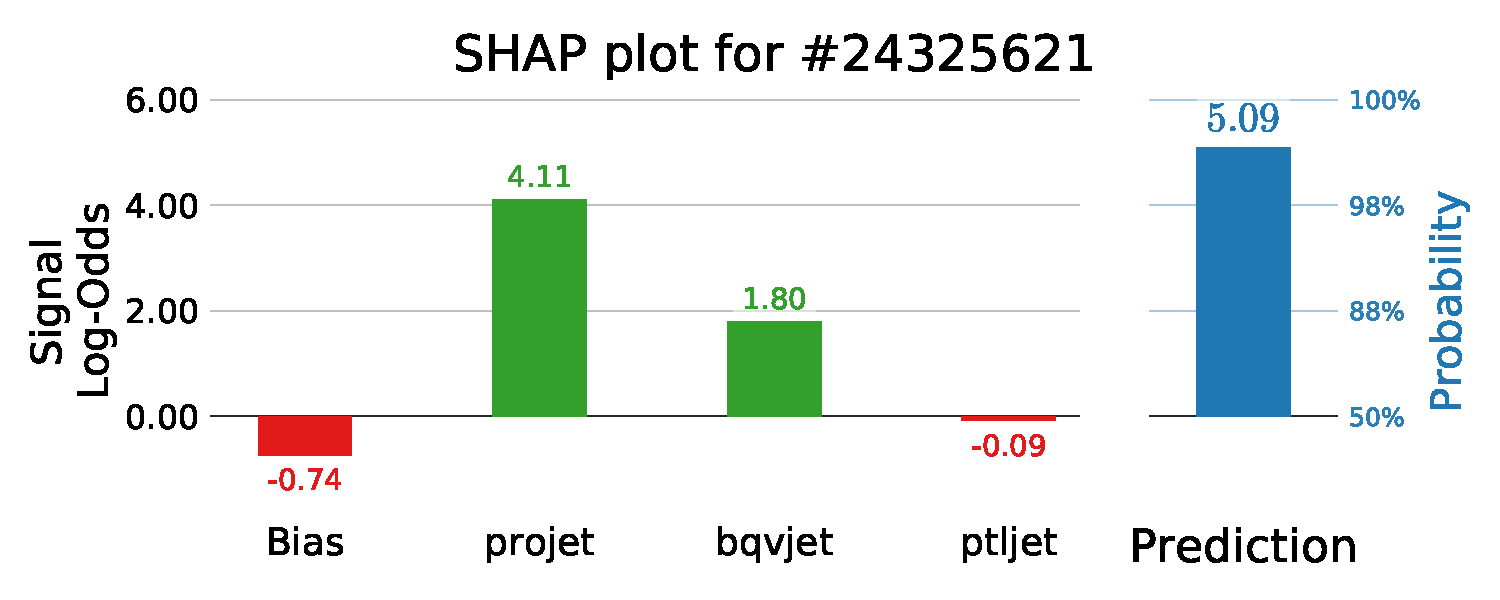
\includegraphics[width=0.95\textwidth, trim=0 0 0 40, clip]{figures/quarks/shap_values-down_sample=1.00-ML_vars=vertex-selection=b-ejet_min=4-n_iter_RS_lgb=99-n_iter_RS_xgb=9-cdot_cut=0.90-version=19-njet=3loc=24325621.pdf}
  \caption[SHAP Prediction Explanation for b-like jet][6pt]
          {Model explanation for the 3-jet b-tagging model for a b-like jet. The first column is the bias of the training set which acts as the naive prediction baseline, the rest are the input data variables. On the right hand side of the plot is the model prediction shown. The left part of the plot is shown in log-odds space, the right part in probability space. The model prediction is the sum of the log-odds (5.09 in this example) transformed into probability space. The \textcolor{red}{negative} log-odd values are shown in red, \textcolor{green}{positive} ones in green, and the \textcolor{blue}{prediction value} in blue. 
          } 
  \label{fig:q:shap_signal}
\end{figure}


\begin{figure}
  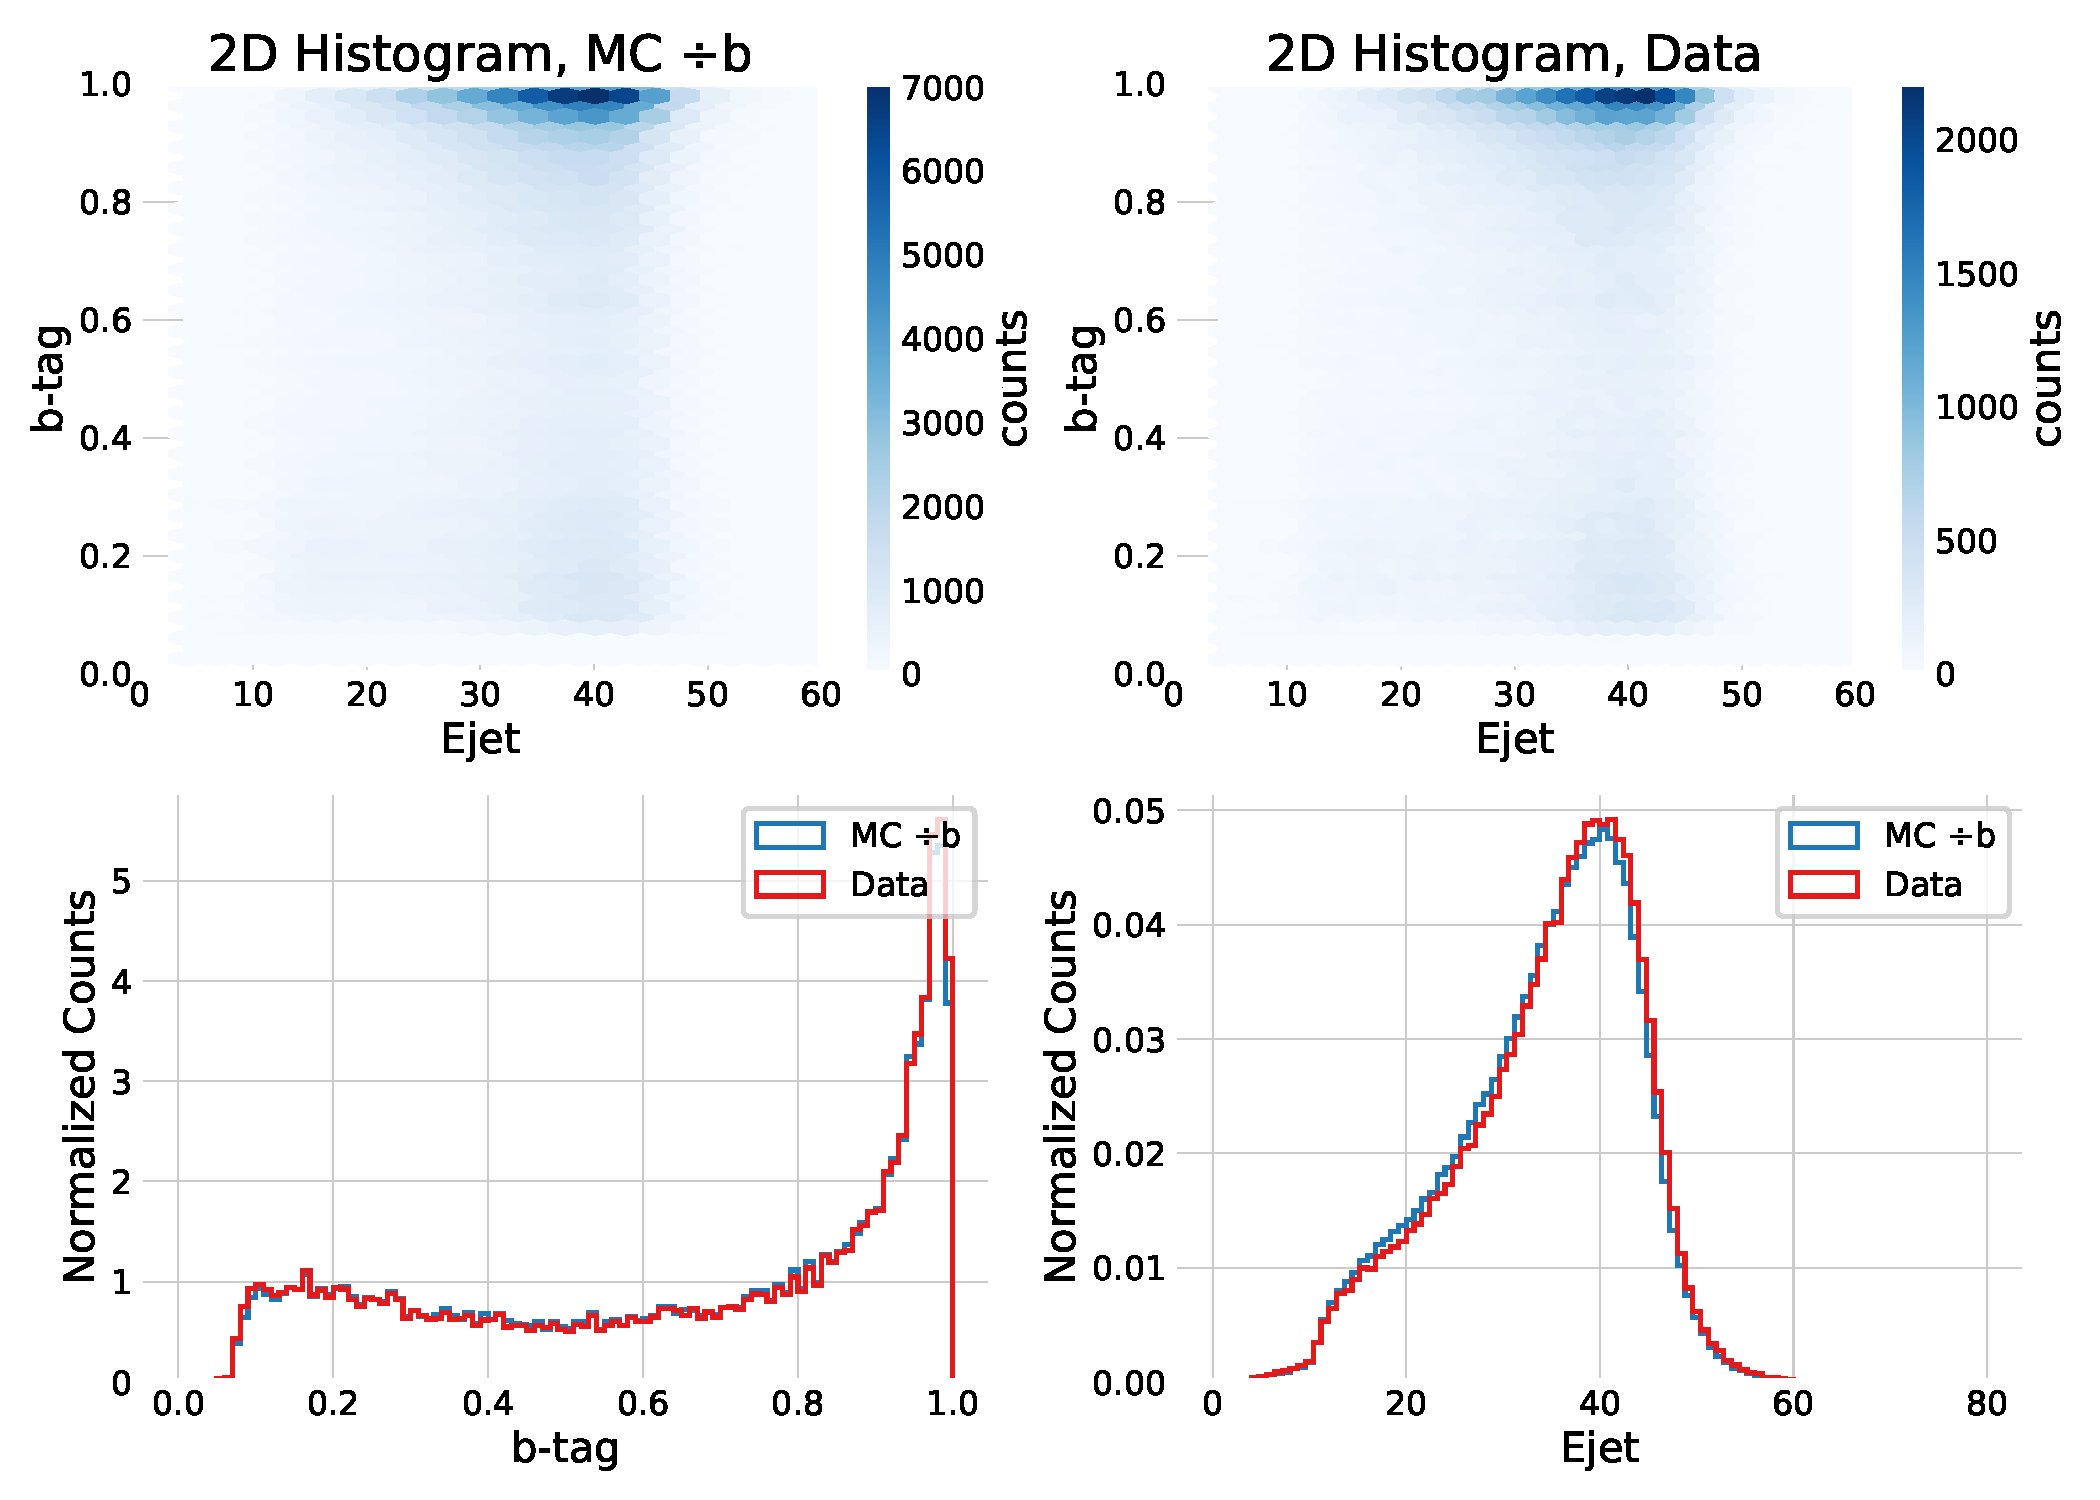
\includegraphics[width=0.95\textwidth, trim=0 0 0 40, clip]{figures/quarks/2d-histograms-ejet-btag-comparison-down_sample=1.00-ML_vars=vertex-selection=b-ejet_min=4-n_iter_RS_lgb=99-n_iter_RS_xgb=9-cdot_cut=0.90-version=19-njet=3.pdf}
  \caption[Monte Carlo -- Data bias for b-tags and jet energy][6pt]
          {Comparison of the b-tag and jet energy (\code{Ejet}) distributions for Monte Carlo (MC) versus data. In the top row the 2D-distributions are shown for MC on the left (without the extra MCb samples) and data on the right. In the bottom row the 1D marginal distrubtions are shown for the b-tag and the jet energy with \textcolor{red}{data} in red and \textcolor{blue}{Monte Carlo} ones in blue. Notice the the almost identical distributions in b-tag. 
          } 
  \label{fig:q:btag_Ejet_comparison}
\end{figure}

\begin{figure}
  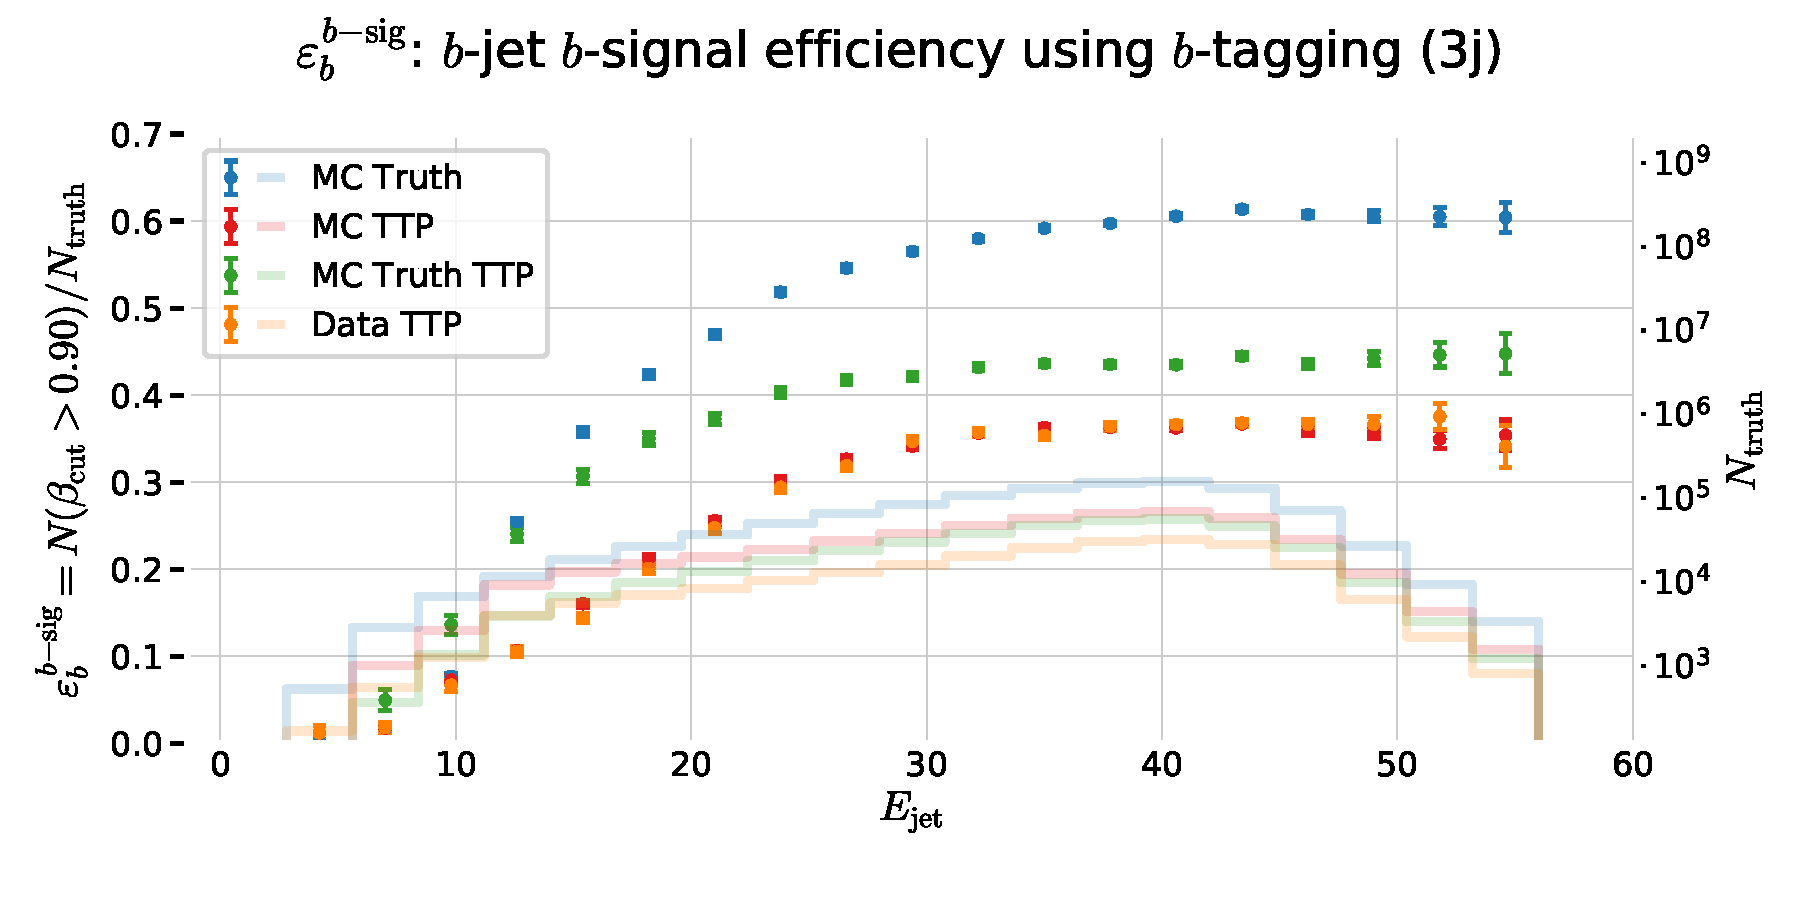
\includegraphics[width=0.95\textwidth, trim=0 0 0 40, clip]{figures/quarks/eff_b_bsig-down_sample=1.00-ML_vars=vertex-selection=b-ejet_min=4-n_iter_RS_lgb=99-n_iter_RS_xgb=9-cdot_cut=0.90-version=19.pdf}
  \caption[b-Tagging Efficiency $\varepsilon_b^{b\mathrm{-sig}}$ as a function of jet energy][6pt]
          {Efficiency of the b-tags for b-jets in the b-signal region for 3-jet events, $\varepsilon_b^{b\mathrm{-sig}}$, as a function of jet energy \code{Ejet}. The b-signal region is defined as $\beta > 0.9$. In the plot the efficiencies are shown for \textcolor{blue}{MC Truth} in blue, \textcolor{red}{MC TTP} in red, \textcolor{green}{MC Truth TTP} in green, and \textcolor{orange}{Data TTP} in orange. The efficiencies (the errorbars) can be read off on the left y-axis and the counts (histograms) on the right y-axis. The abbreviation TTP is short for \q{Tag, Tag, Probe} where two jets in a event are used as tags and the probe is then used for further analysis. Notice how both MC TTP and Data TTP follow each other closely.  
          } 
  \label{fig:q:effiency_btag_bjet_bsig}
\end{figure}


\begin{figure}
  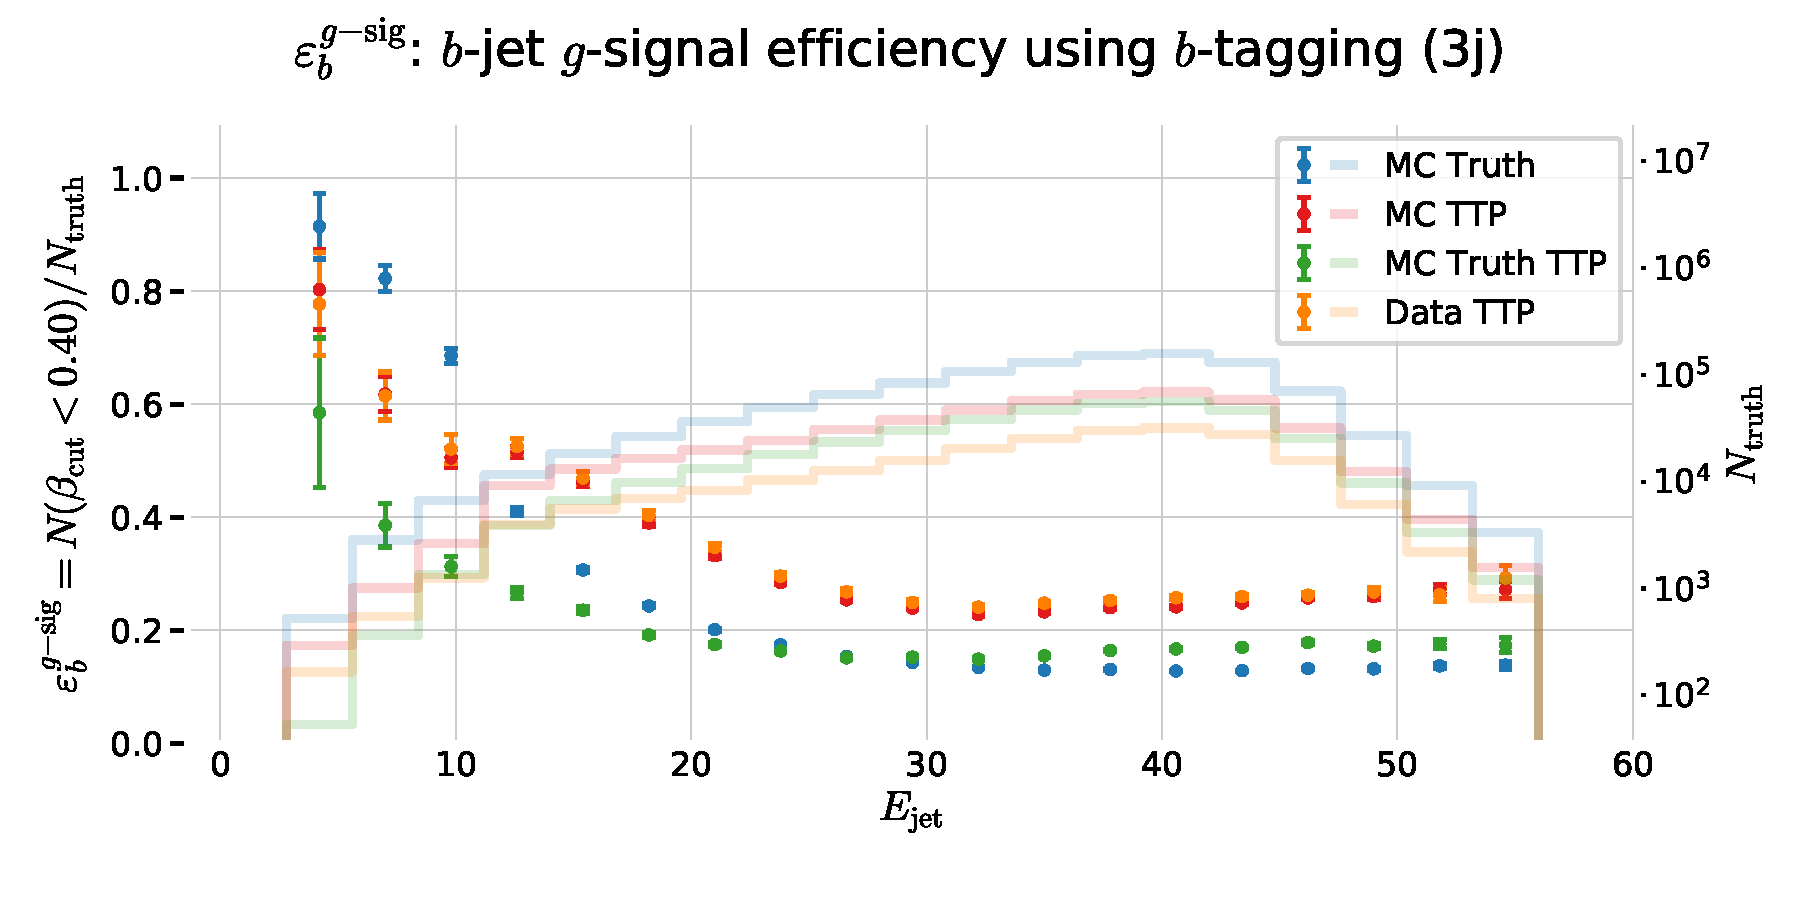
\includegraphics[width=0.95\textwidth, trim=0 0 0 40, clip]{figures/quarks/eff_b_gsig-down_sample=1.00-ML_vars=vertex-selection=b-ejet_min=4-n_iter_RS_lgb=99-n_iter_RS_xgb=9-cdot_cut=0.90-version=19.pdf}
  \caption[b-Tagging Efficiency $\varepsilon_b^{g\mathrm{-sig}}$ as a function of jet energy][6pt]
          {Efficiency of the b-tags for b-jets in the g-signal region for 3-jet events, $\varepsilon_b^{g\mathrm{-sig}}$, as a function of jet energy \code{Ejet}. The g-signal region is defined as $\beta < 0.4$. In the plot the efficiencies are shown for \textcolor{blue}{MC Truth} in blue, \textcolor{red}{MC TTP} in red, \textcolor{green}{MC Truth TTP} in green, and \textcolor{orange}{Data TTP} in orange. The efficiencies (the errorbars) can be read off on the left y-axis and the counts (histograms) on the right y-axis. The abbreviation TTP is short for \q{Tag, Tag, Probe} where two jets in a event are used as tags and the probe is then used for further analysis. Notice how both MC TTP and Data TTP follow each other closely.  
          } 
  \label{fig:q:effiency_btag_bjet_gsig}
\end{figure}


\begin{figure}
  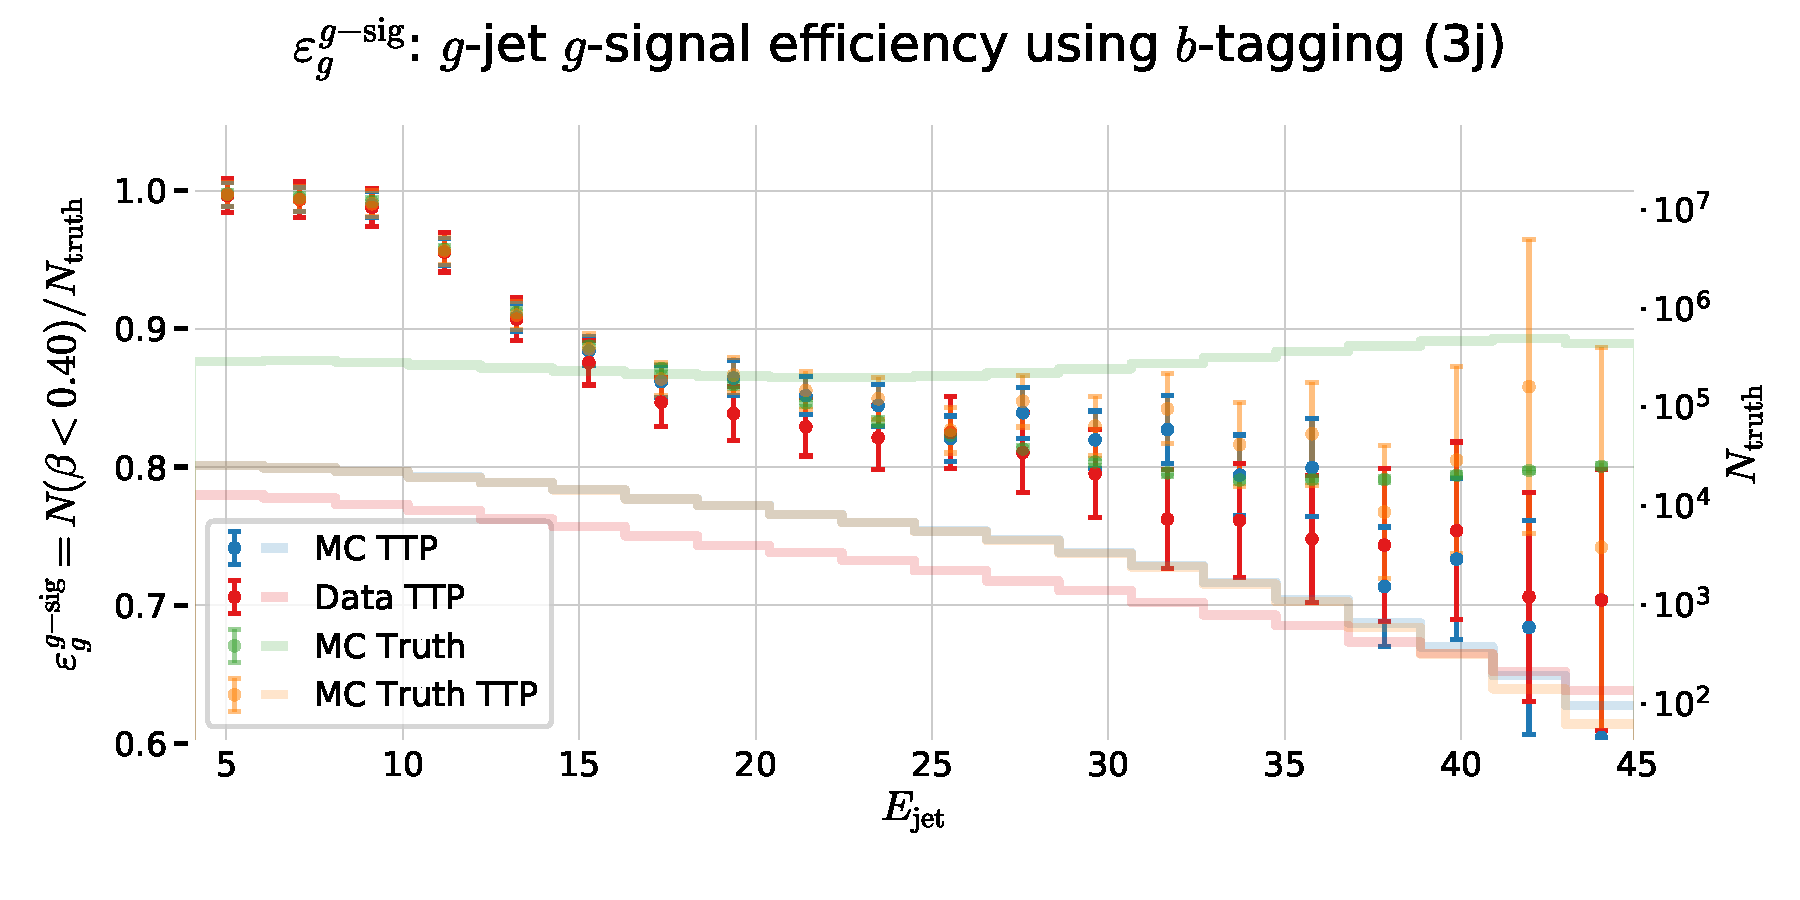
\includegraphics[width=0.95\textwidth, trim=0 0 0 40, clip]{figures/quarks/eff_g_gsig-down_sample=1.00-ML_vars=vertex-selection=b-ejet_min=4-n_iter_RS_lgb=99-n_iter_RS_xgb=9-cdot_cut=0.90-version=19.pdf}
  \caption[b-Tagging Efficiency $\varepsilon_g^{g\mathrm{-sig}}$ as a function of jet energy][6pt]
          {Efficiency of the b-tags for g-jets in the g-signal region for 3-jet events, $\varepsilon_g^{g\mathrm{-sig}}$, as a function of jet energy \code{Ejet}. The g-signal region is defined as $\beta < 0.4$. In the plot the efficiencies are shown for \textcolor{blue}{MC Truth} in blue, \textcolor{red}{MC TTP} in red, \textcolor{green}{MC Truth TTP} in green, and \textcolor{orange}{Data TTP} in orange. The efficiencies (the errorbars) can be read off on the left y-axis and the counts (histograms) on the right y-axis. The abbreviation TTP is short for \q{Tag, Tag, Probe} where two jets in a event are used as tags and the probe is then used for further analysis. Notice how both MC TTP and Data TTP follow each other closely.  
          } 
  \label{fig:q:effiency_btag_gjet_gsig}
\end{figure}

\begin{figure}
  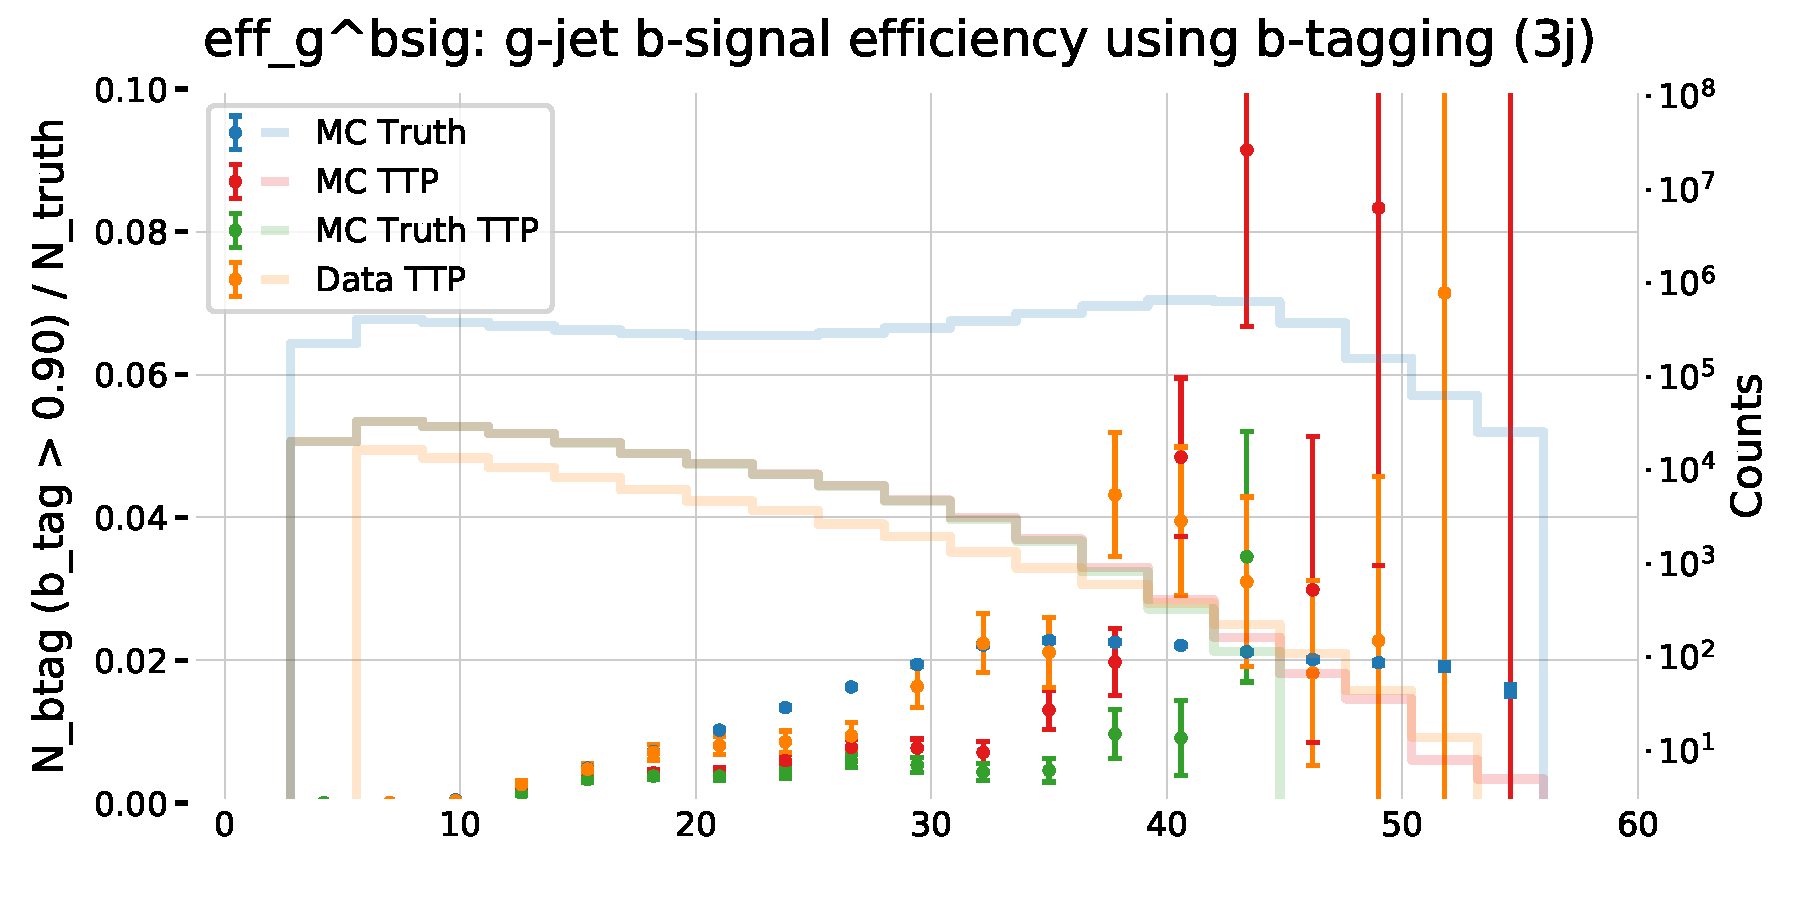
\includegraphics[width=0.95\textwidth, trim=0 0 0 30, clip]{figures/quarks/eff_g_bsig-down_sample=1.00-ML_vars=vertex-selection=b-ejet_min=4-n_iter_RS_lgb=99-n_iter_RS_xgb=9-cdot_cut=0.90-version=19.pdf}
  \caption[b-Tagging Efficiency $\varepsilon_g^{b\mathrm{-sig}}$ as a function of jet energy][6pt]
          {Efficiency of the b-tags for g-jets in the b-signal region for 3-jet events, $\varepsilon_g^{b\mathrm{-sig}}$, as a function of jet energy \code{Ejet}. The b-signal region is defined as $\beta > 0.9$. In the plot the efficiencies are shown for \textcolor{blue}{MC Truth} in blue, \textcolor{red}{MC TTP} in red, \textcolor{green}{MC Truth TTP} in green, and \textcolor{orange}{Data TTP} in orange. The efficiencies (the errorbars) can be read off on the left y-axis and the counts (histograms) on the right y-axis. The abbreviation TTP is short for \q{Tag, Tag, Probe} where two jets in a event are used as tags and the probe is then used for further analysis.  
          } 
  \label{fig:q:effiency_btag_gjet_bsig}
\end{figure}


\begin{figure}
  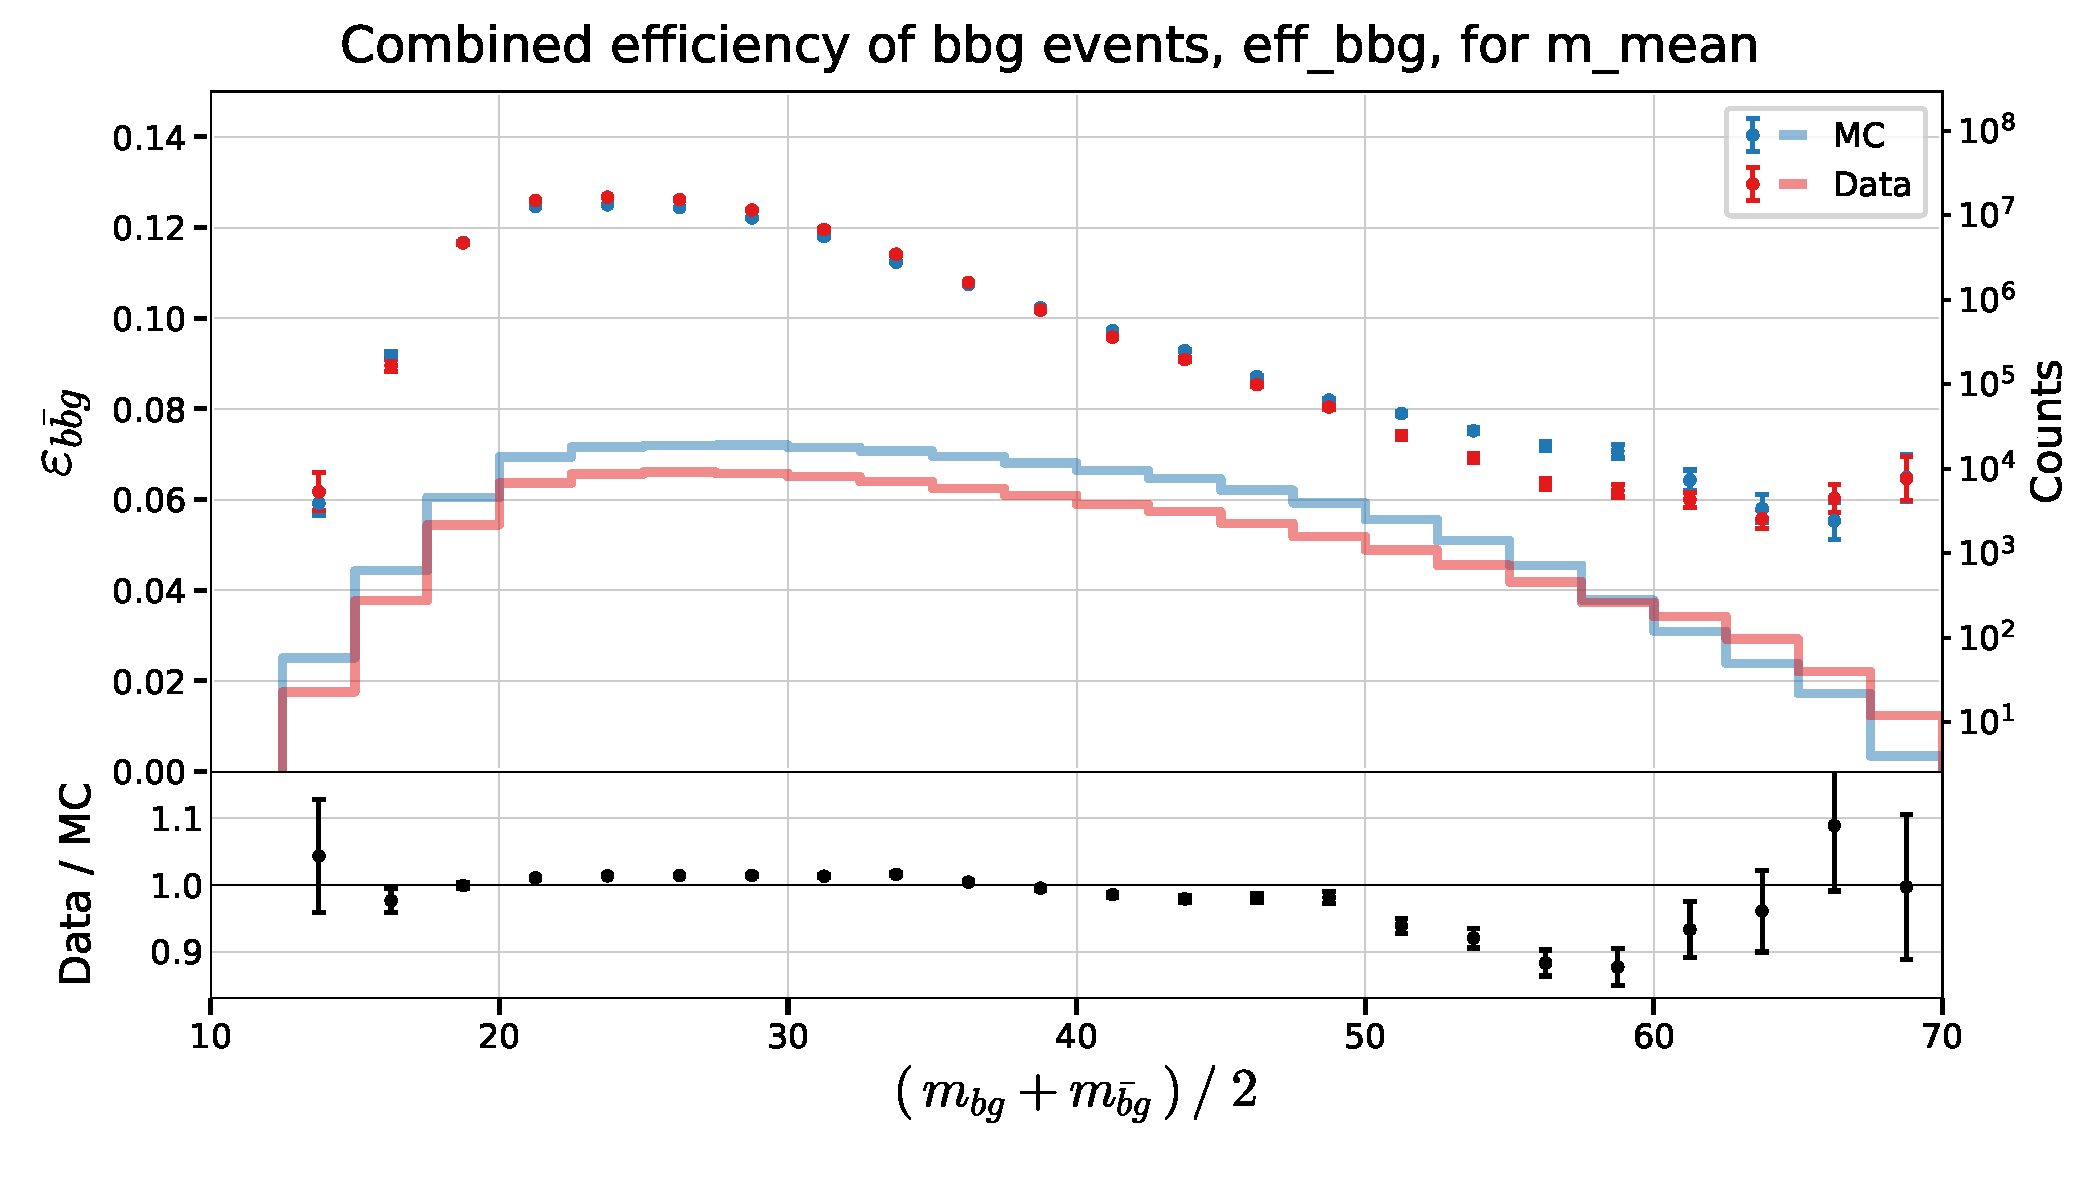
\includegraphics[width=0.95\textwidth, trim=0 0 0 40, clip]{figures/quarks/eff_bbg_m_mean-down_sample=1.00-ML_vars=vertex-selection=b-ejet_min=4-n_iter_RS_lgb=99-n_iter_RS_xgb=9-cdot_cut=0.90-version=19.pdf}
  \caption[g-Tagging proxy efficiency for $b\bar{b}g$-events as function of the mean invariant mass][6pt]
          {Proxy efficiency of the g-tags for $b\bar{b}g$ 3-jet events as a function of the mean of the two invariant masses $m_{bg}$ and $m_{\bar{b}g}$. The proxy efficiency $\varepsilon_{b\bar{b}g}$ is measured by finding $b\bar{b}g$-events where $\beta_b > 0.9$, $\beta_{\bar{b}}>0.9$, and $\beta_g < 0.4$. and then calculating  $\varepsilon_{b\bar{b}g} = \varepsilon_b^{b\mathrm{-sig}} \cdot \varepsilon_{\bar{b}}^{b\mathrm{-sig}} \cdot  \varepsilon_g^{g\mathrm{-sig}} $. In the top plot $\varepsilon_{b\bar{b}g}$ is shown for \textcolor{blue}{MC} in blue and \textcolor{red}{Data} in red where the counts in each bin can be read on right y-axis. In the bottom plot the ratio between Data and MC is shown.
          } 
  \label{fig:q:effiency_btag_bbg_m_mean}
\end{figure}


\begin{figure}
  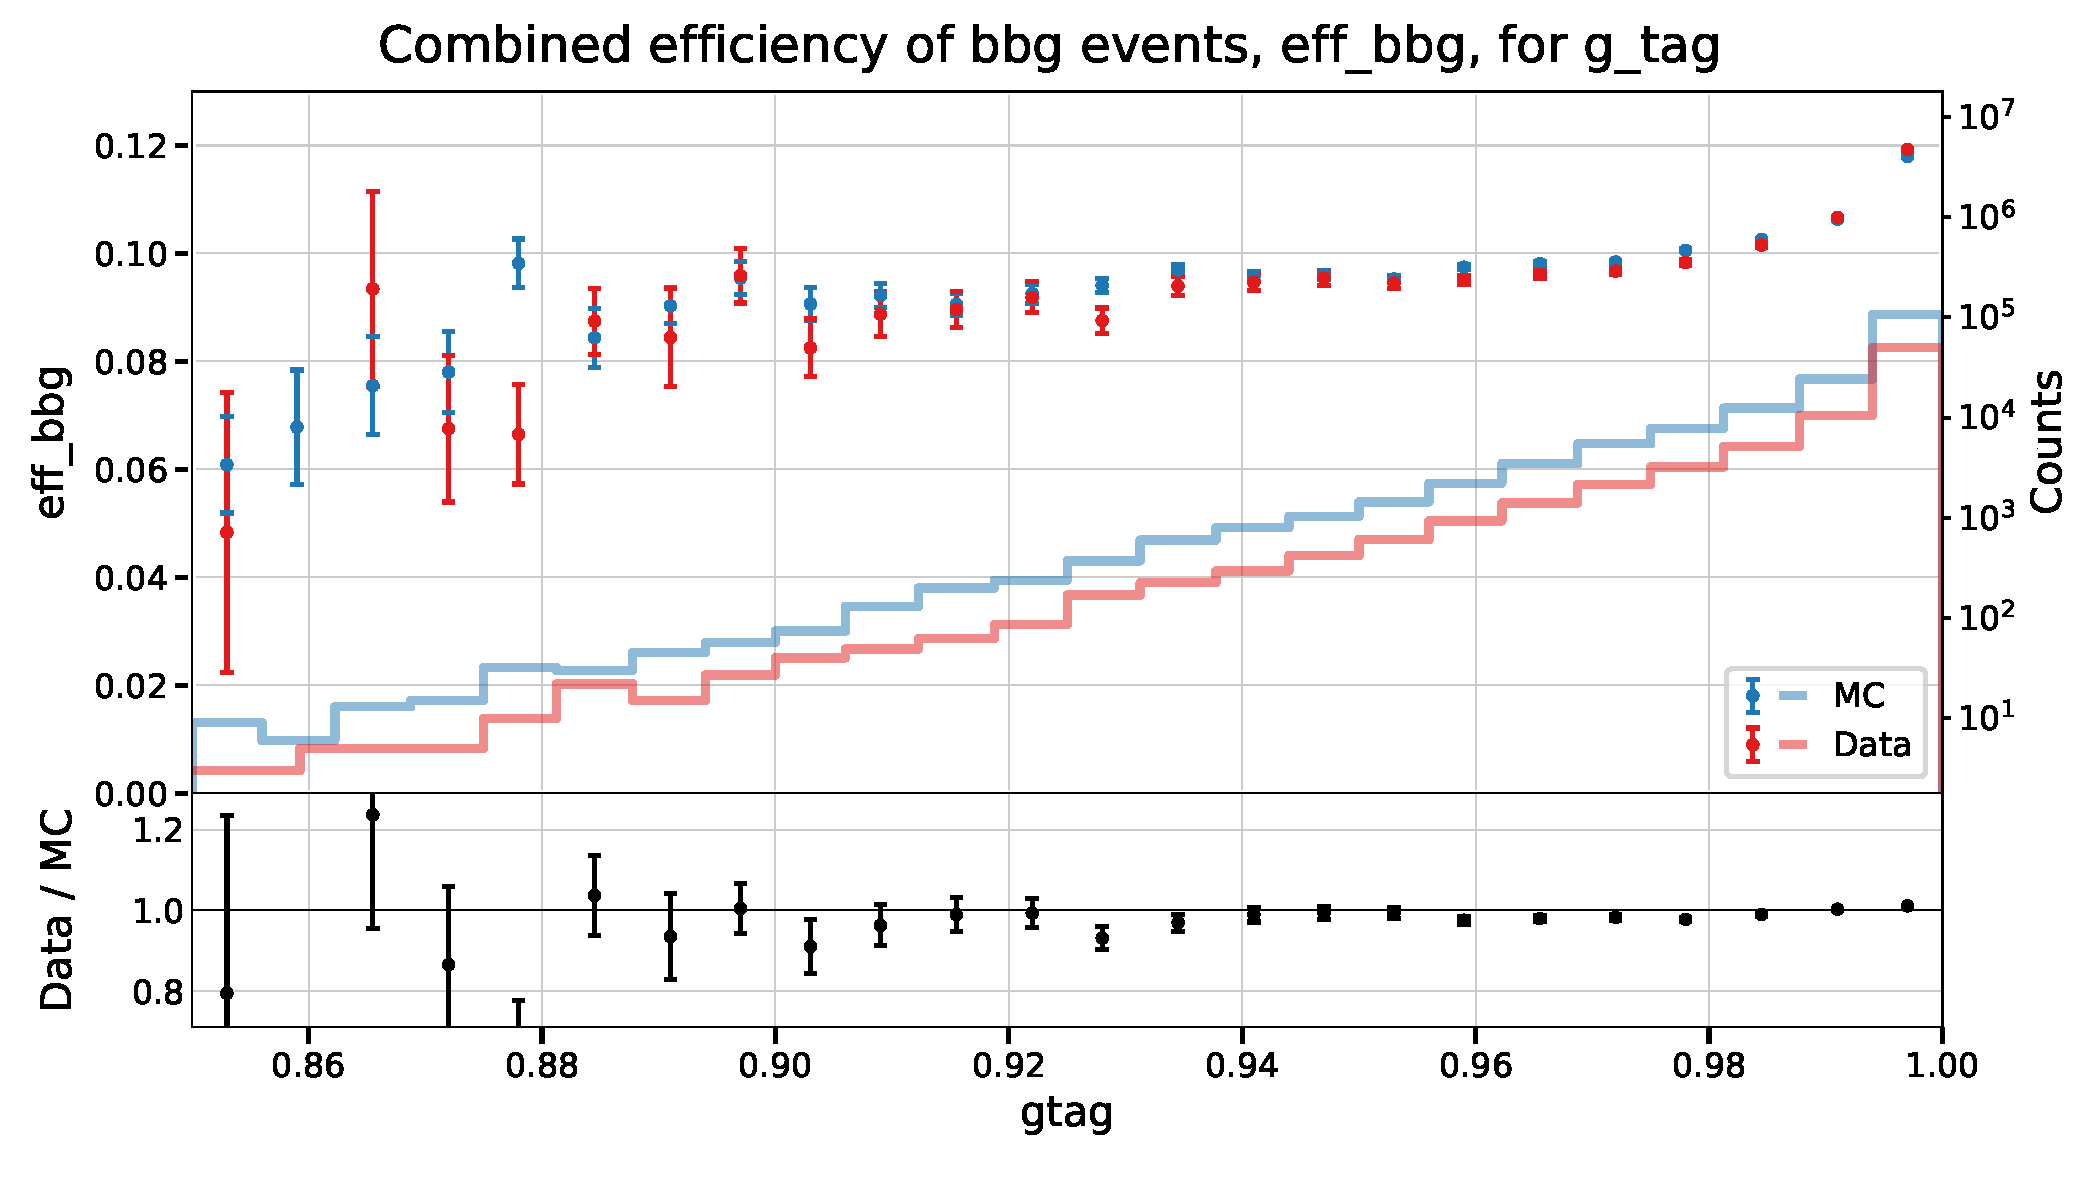
\includegraphics[width=0.95\textwidth, trim=0 0 0 40, clip]{figures/quarks/eff_bbg_gtag-down_sample=1.00-ML_vars=vertex-selection=b-ejet_min=4-n_iter_RS_lgb=99-n_iter_RS_xgb=9-cdot_cut=0.90-version=19.pdf}
  \caption[g-Tagging proxy efficiency for $b\bar{b}g$-events as function of g-tag][6pt]
          {Proxy efficiency of the g-tags for $b\bar{b}g$ 3-jet events as a function of the event's g-tag. The proxy efficiency $\varepsilon_{b\bar{b}g}$ is measured by finding $b\bar{b}g$-events where $\beta_b > 0.9$, $\beta_{\bar{b}}>0.9$, and $\beta_g < 0.4$. and then calculating  $\varepsilon_{b\bar{b}g} = \varepsilon_b^{b\mathrm{-sig}} \cdot \varepsilon_{\bar{b}}^{b\mathrm{-sig}} \cdot  \varepsilon_g^{g\mathrm{-sig}} $. In the top plot $\varepsilon_{b\bar{b}g}$ is shown for \textcolor{blue}{MC} in blue and \textcolor{red}{Data} in red where the counts in each bin can be read on right y-axis. In the bottom plot the ratio between Data and MC is shown.
          } 
  \label{fig:q:effiency_btag_bbg_gtag}
\end{figure}



\begin{figure}
  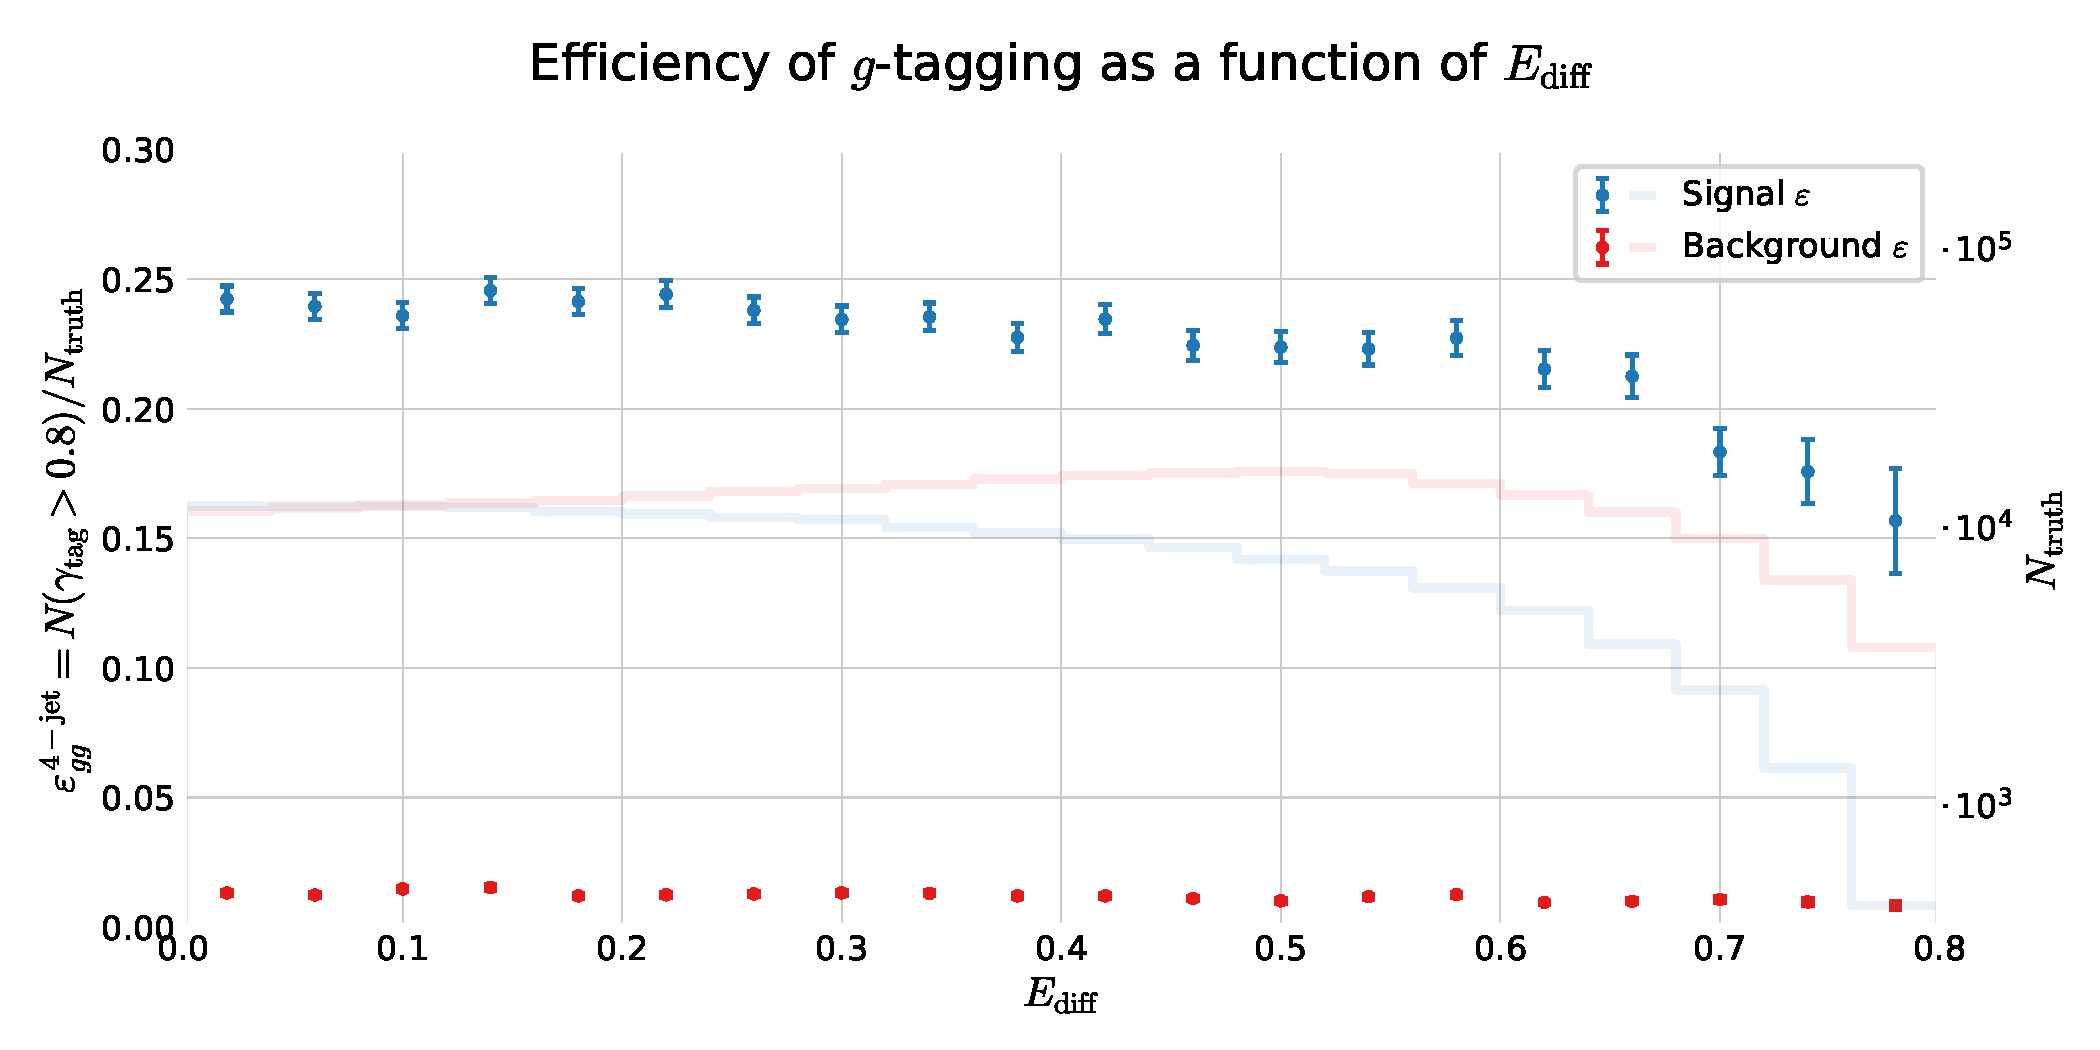
\includegraphics[width=0.95\textwidth, trim=0 0 0 40, clip, page=1]{figures/quarks/efficiency_events-down_sample=1.00-ML_vars=vertex-selection=b-ejet_min=4-n_iter_RS_lgb=99-n_iter_RS_xgb=9-cdot_cut=0.90-version=19-njet=4.pdf}
  \caption[g-Tagging efficiency for 4-jet events in MC as a function of normalized gluon gluon jet energy difference][6pt]
          {Efficiency of the g-tags for 4-jet events as a function of normalized gluon gluon jet energy difference in Monte Carlo. The efficiency is measured as the number of events with a g-tag higher than 0.8 ($\gamma > 0.8$) out of the total number and the normalized gluon gluon jet energy difference $A$ is $A=\frac{E_{g_\mathrm{max}}-E_{g_\mathrm{min}}}{E_{g_\mathrm{max}}+E_{g_\mathrm{min}}}$ where $E_{g_\mathrm{max}}$ ($E_{g_\mathrm{min}}$) refers to the energy of the gluon with the highest (lowest) energy. The efficiency is plotted for \textcolor{blue}{signal events} according to MC Truth in blue and \textcolor{red}{background events} according to MC Truth in red.
          } 
  \label{fig:q:effiency_gtag_E_diff}
\end{figure}


\begin{figure}
  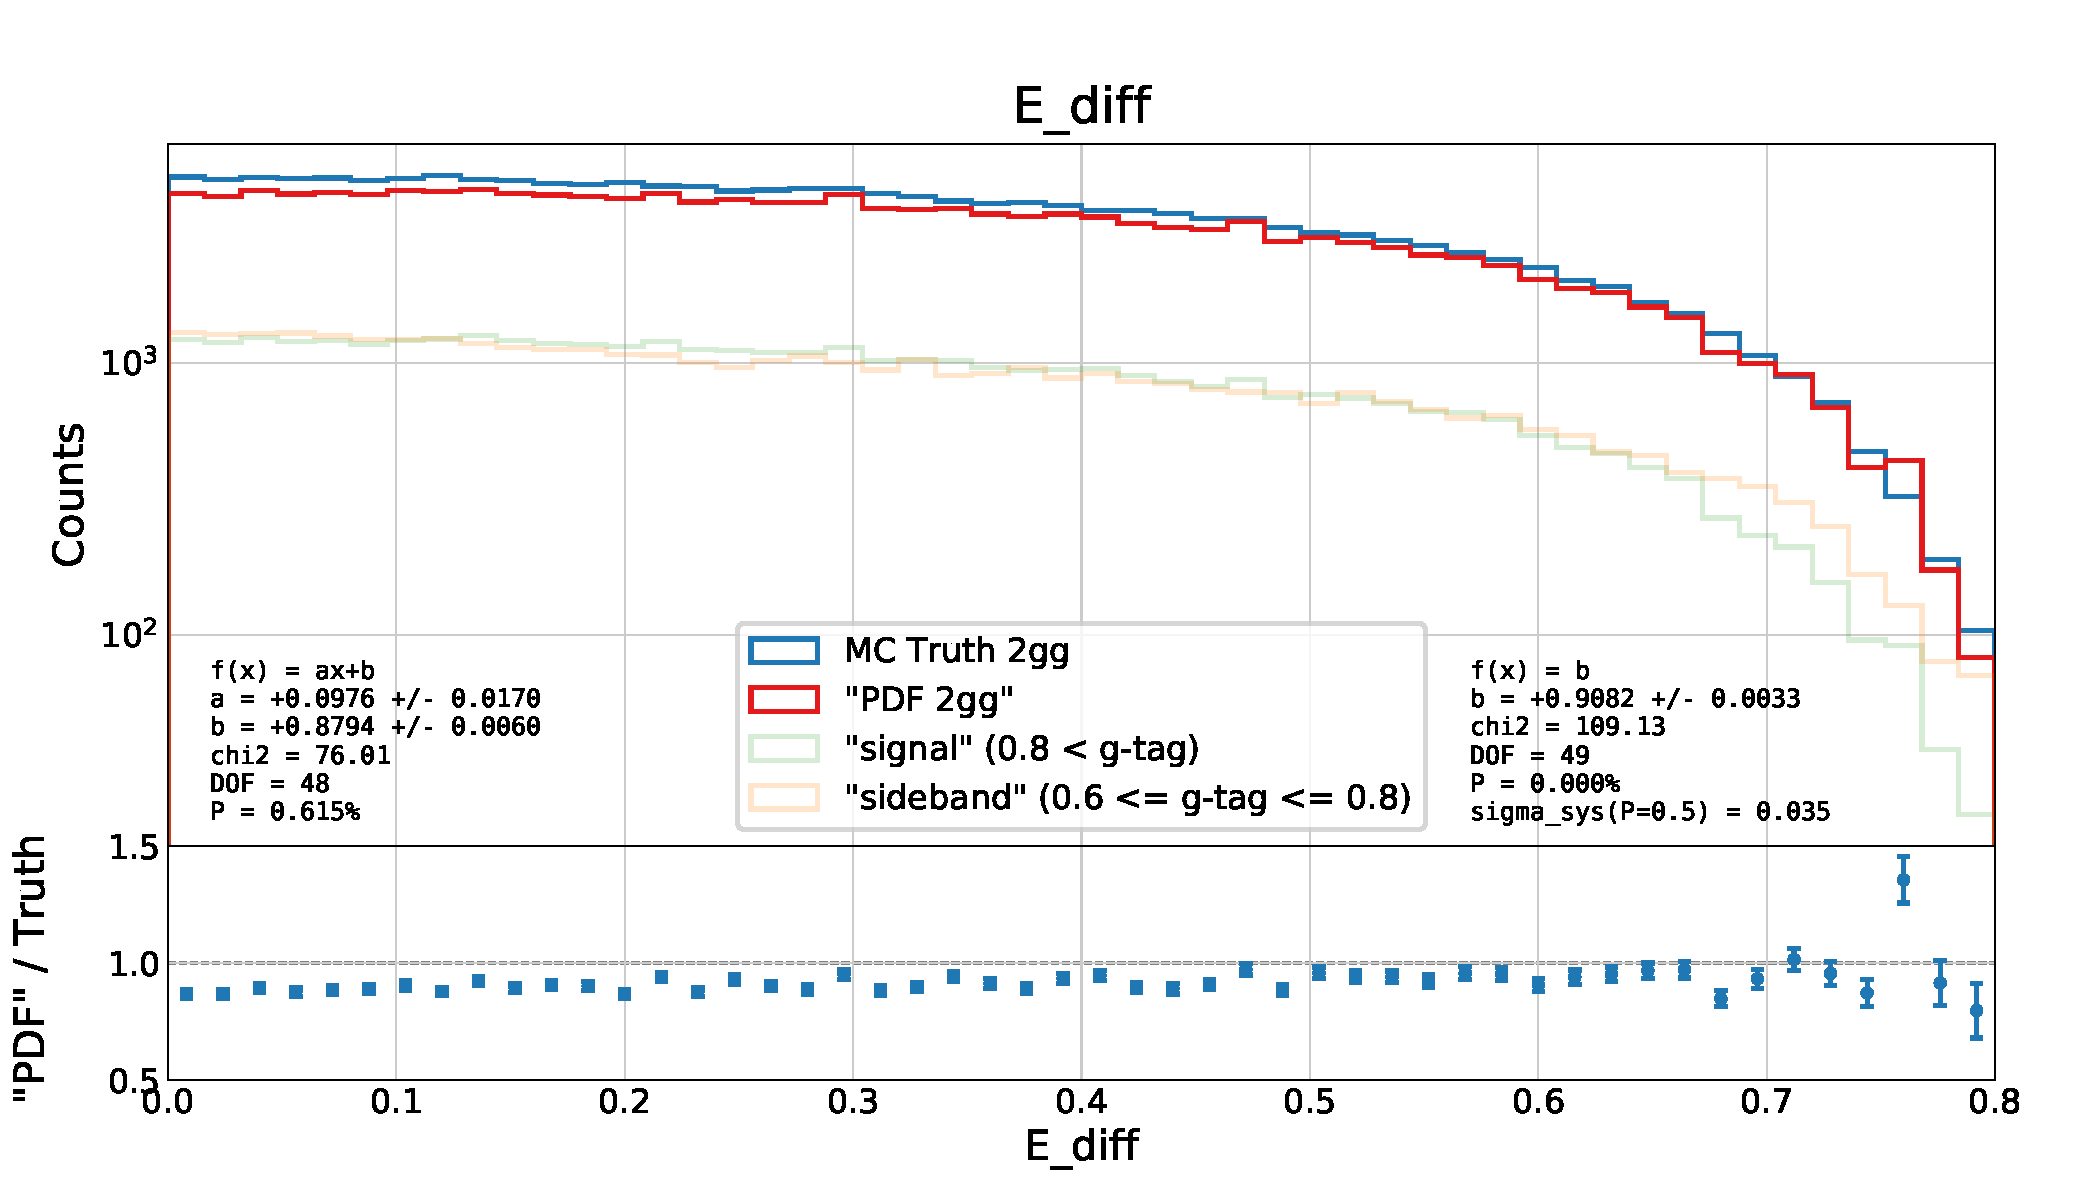
\includegraphics[width=0.95\textwidth, trim=0 0 0 65, clip, page=1]{figures/quarks/gtag-closure_test-down_sample=1.00-ML_vars=vertex-selection=b-ejet_min=4-n_iter_RS_lgb=99-n_iter_RS_xgb=9-cdot_cut=0.90-version=19-njet=3.pdf}
  \caption[Closure plot between MC Truth and the corrected g-tagging model in 4-jet events for the normalized gluon gluon jet energy difference][6pt]
          {Closure plot between MC Truth and the corrected g-tagging model in 4-jet events for the normalized gluon gluon jet energy difference. The corrected g-taggingg model is described in further detail in section XXX \TODO. In the top part of the plot the \textcolor{blue}{MC Truth} is shown in blue, the \textcolor{red}{corrected g-tagging model} \code{"PDF 2gg"} in red, the \textcolor{green}{g-signal distribution} in semi-transparent green and the \textcolor{orange}{g-sideband distribution} in semi-transparent orange. In the bottom part of the plot the ratio between MC Truth and the output of the corrected g-tagging model is shown. The normalized gluon gluon jet energy difference $A$ is $A=\frac{E_{g_\mathrm{max}}-E_{g_\mathrm{min}}}{E_{g_\mathrm{max}}+E_{g_\mathrm{min}}}$ where $E_{g_\mathrm{max}}$ ($E_{g_\mathrm{min}}$) refers to the energy of the gluon with the highest (lowest) energy.
          } 
  \label{fig:q:closure_E_diff}
\end{figure}


\begin{figure}
  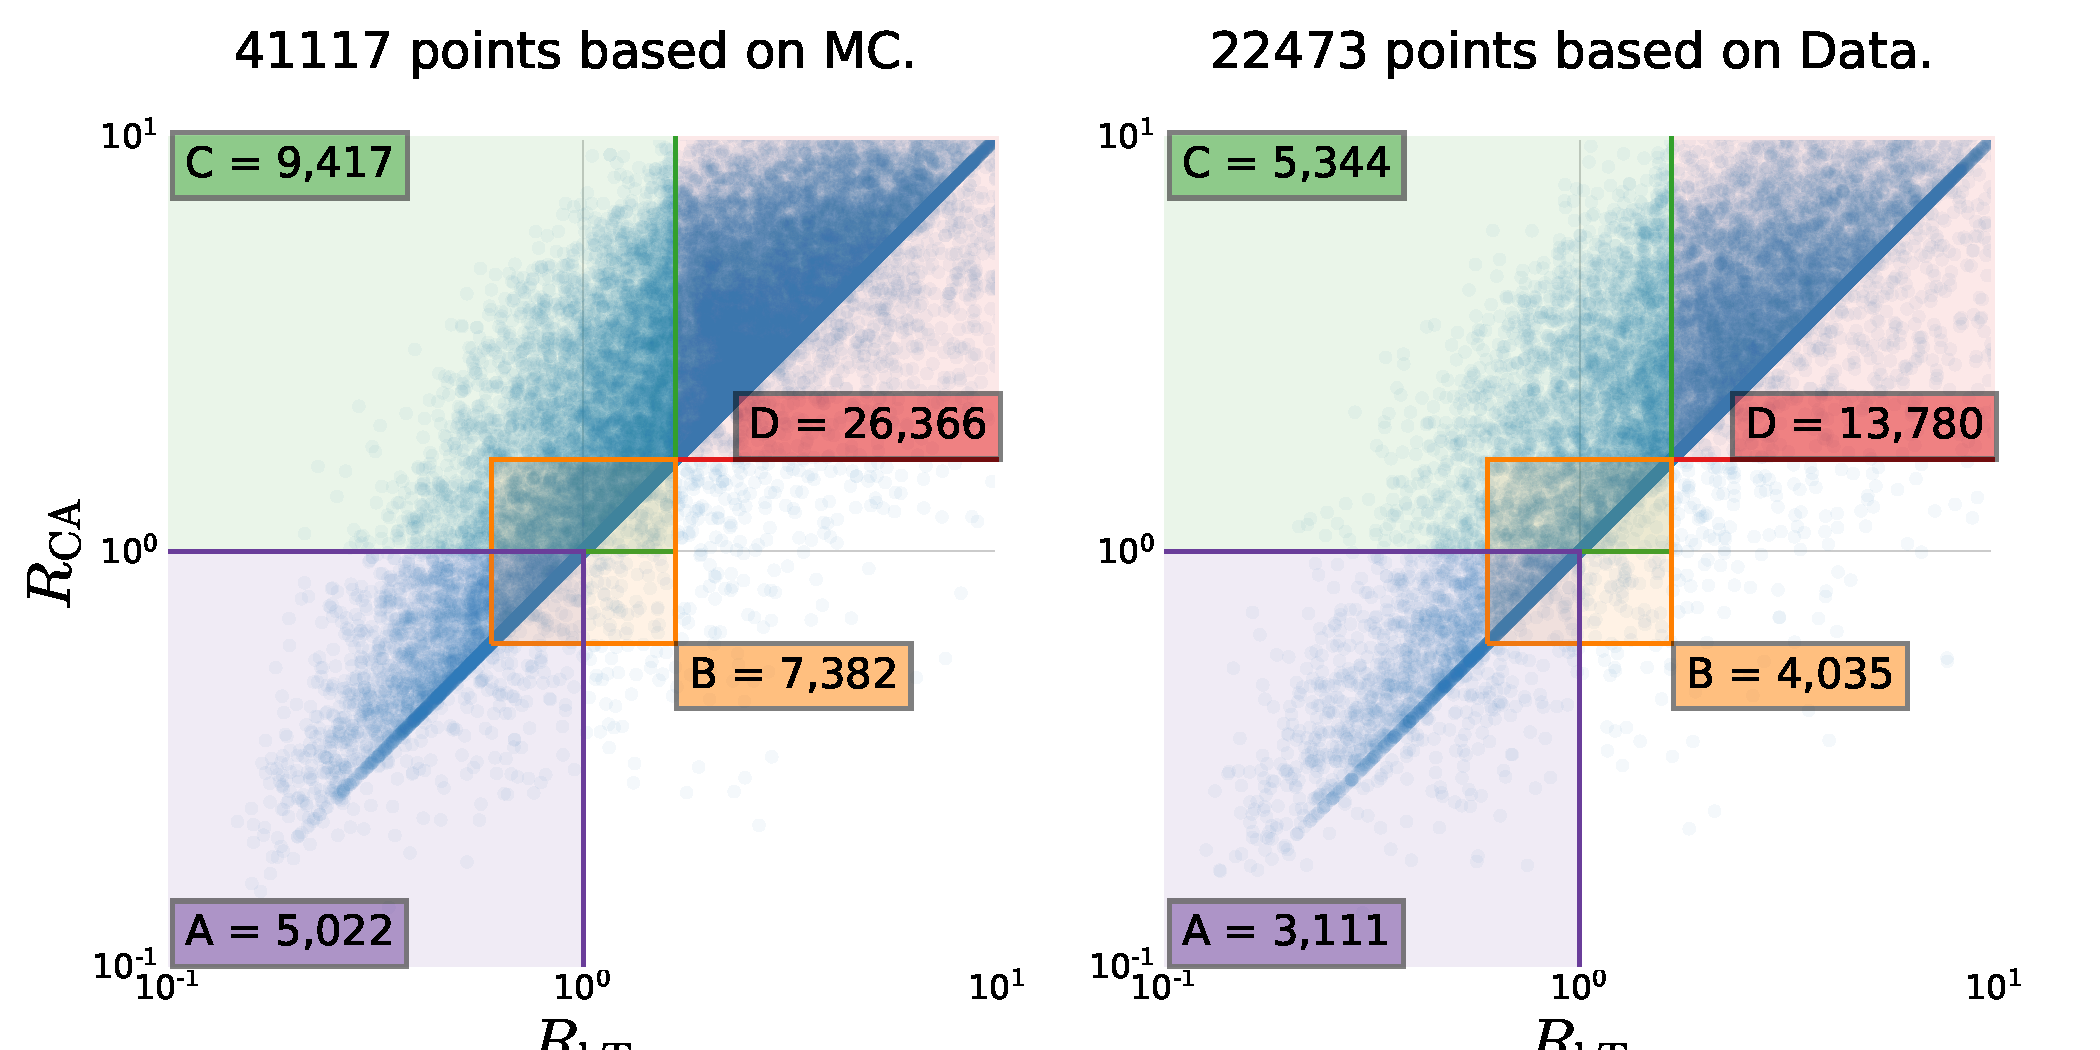
\includegraphics[width=0.95\textwidth, trim=0 0 0 118, clip, page=1]{figures/quarks/gtag-R_kt_CA_overview-down_sample=1.00-ML_vars=vertex-selection=b-ejet_min=4-n_iter_RS_lgb=99-n_iter_RS_xgb=9-cdot_cut=0.90-version=19-njet=4}
  \caption[R kt CA overview  XXX \TODO][6pt]
          {R kt CA overview XXX \TODO
          } 
  \label{fig:q:R_kt_CA_overview}
\end{figure}

\begin{figure}
  \includegraphics[width=0.95\textwidth, trim=0 0 0 30, clip, page=2]{figures/quarks/gtag-R_kt_CA_overview-down_sample=1.00-ML_vars=vertex-selection=b-ejet_min=4-n_iter_RS_lgb=99-n_iter_RS_xgb=9-cdot_cut=0.90-version=19-njet=4}
  \caption[R kt CA cut region A  XXX \TODO][6pt]
          {R kt CA cut region A XXX \TODO
          } 
  \label{fig:q:R_kt_CA_cut_A}
\end{figure}


The specification of the \doccmddef{sidenote} command is:
\begin{docspec}
  \doccmd{sidenote}[\docopt{number}][\docopt{offset}]\{\docarg{Sidenote text.}\}
\end{docspec}

Both the \docopt{number} and \docopt{offset} arguments are optional.  If you
provide a \docopt{number} argument, then that number will be used as the
sidenote number.  It will change of the number of the current sidenote only and
will not affect the numbering sequence of subsequent sidenotes.

Sometimes a sidenote may run over the top of other text or graphics in the
margin space.  If this happens, you can adjust the vertical position of the
sidenote by providing a dimension in the \docopt{offset} argument.  Some
examples of valid dimensions are:
\begin{docspec}
  \ttfamily 1.0in \qquad 2.54cm \qquad 254mm \qquad 6\Verb|\baselineskip|
\end{docspec}
If the dimension is positive it will push the sidenote down the page; if the
dimension is negative, it will move the sidenote up the page.

While both the \docopt{number} and \docopt{offset} arguments are optional, they
must be provided in order.  To adjust the vertical position of the sidenote
while leaving the sidenote number alone, use the following syntax:
\begin{docspec}
  \doccmd{sidenote}[][\docopt{offset}]\{\docarg{Sidenote text.}\}
\end{docspec}
The empty brackets tell the \Verb|\sidenote| command to use the default
sidenote number.

If you \emph{only} want to change the sidenote number, however, you may
completely omit the \docopt{offset} argument:
\begin{docspec}
  \doccmd{sidenote}[\docopt{number}]\{\docarg{Sidenote text.}\}
\end{docspec}

The \doccmddef{marginnote} command has a similar \docarg{offset} argument:
\begin{docspec}
  \doccmd{marginnote}[\docopt{offset}]\{\docarg{Margin note text.}\}
\end{docspec}

\section{References}
References are placed alongside their citations as sidenotes,
as well.  This can be accomplished using the normal \doccmddef{cite}
command.\sidenote{The first paragraph of this document includes a citation.}

The complete list of references may also be printed automatically by using
the \doccmddef{bibliography} command.  (See the end of this document for an
example.)  If you do not want to print a bibliography at the end of your
document, use the \doccmddef{nobibliography} command in its place.  


\section{Figures and Tables}\label{sec:figures-and-tables}
Images and graphics play an integral role in Tufte's work.
In addition to the standard \docenvdef{figure} and \docenvdef{tabular} environments,
this style provides special figure and table environments for full-width
floats.

Full page--width figures and tables may be placed in \docenvdef{figure*} or
\docenvdef{table*} environments.  To place figures or tables in the margin,
use the \docenvdef{marginfigure} or \docenvdef{margintable} environments as follows
(see figure~\ref{fig:marginfig}):

\begin{marginfigure}%
  \includegraphics[width=\linewidth]{helix}
  \caption{This is a margin figure.  The helix is defined by 
    $x = \cos(2\pi z)$, $y = \sin(2\pi z)$, and $z = [0, 2.7]$.  The figure was
    drawn using Asymptote (\url{http://asymptote.sf.net/}).}
  \label{fig:marginfig}
\end{marginfigure}

\begin{docspec}
\textbackslash begin\{marginfigure\}\\
  \qquad\textbackslash includegraphics\{helix\}\\
  \qquad\textbackslash caption\{This is a margin figure.\}\\
  \qquad\textbackslash label\{fig:marginfig\}\\
\textbackslash end\{marginfigure\}\\
\end{docspec}

The \docenv{marginfigure} and \docenv{margintable} environments accept an optional parameter \docopt{offset} that adjusts the vertical position of the figure or table.  See the ``\nameref{sec:sidenotes}'' section above for examples.  The specifications are:
\begin{docspec}
  \textbackslash{begin\{marginfigure\}[\docopt{offset}]}\\
  \qquad\ldots\\
  \textbackslash{end\{marginfigure\}}\\
  \mbox{}\\
  \textbackslash{begin\{margintable\}[\docopt{offset}]}\\
  \qquad\ldots\\
  \textbackslash{end\{margintable\}}\\
\end{docspec}

Figure~\ref{fig:fullfig} is an example of the \docenv{figure*}
environment and figure~\ref{fig:textfig} is an example of the normal
\docenv{figure} environment.

\begin{figure*}[h]
  \includegraphics[width=\linewidth]{sine.pdf}%
  \caption{This graph shows $y = \sin x$ from about $x = [-10, 10]$.
  \emph{Notice that this figure takes up the full page width.}}%
  \label{fig:fullfig}%
\end{figure*}

\begin{figure}
  \includegraphics{hilbertcurves.pdf}
%  \checkparity This is an \pageparity\ page.%
  \caption[Hilbert curves of various degrees $n$.][6pt]{Hilbert curves of various degrees $n$. \emph{Notice that this figure only takes up the main textblock width.}}
  \label{fig:textfig}
  %\zsavepos{pos:textfig}
\end{figure}

As with sidenotes and marginnotes, a caption may sometimes require vertical
adjustment. The \doccmddef{caption} command now takes a second optional
argument that enables you to do this by providing a dimension \docopt{offset}.
You may specify the caption in any one of the following forms:
\begin{docspec}
  \doccmd{caption}\{\docarg{long caption}\}\\
  \doccmd{caption}[\docarg{short caption}]\{\docarg{long caption}\}\\
  \doccmd{caption}[][\docopt{offset}]\{\docarg{long caption}\}\\
  \doccmd{caption}[\docarg{short caption}][\docopt{offset}]%
                  \{\docarg{long caption}\}
\end{docspec}
A positive \docopt{offset} will push the caption down the page. The short
caption, if provided, is what appears in the list of figures/tables, otherwise
the ``long'' caption appears there. Note that although the arguments
\docopt{short caption} and \docopt{offset} are both optional, they must be
provided in order. Thus, to specify an \docopt{offset} without specifying a
\docopt{short caption}, you must include the first set of empty brackets
\Verb|[]|, which tell \doccmd{caption} to use the default ``long'' caption. As
an example, the caption to figure~\ref{fig:textfig} above was given in the form
\begin{docspec}
  \doccmd{caption}[Hilbert curves...][6pt]\{Hilbert curves...\}
\end{docspec}

Table~\ref{tab:normaltab} shows table created with the \docpkg{booktabs}
package.  Notice the lack of vertical rules---they serve only to clutter
the table's data.

\begin{table}[ht]
  \centering
  \fontfamily{ppl}\selectfont
  \begin{tabular}{ll}
    \toprule
    Margin & Length \\
    \midrule
    Paper width & \unit[8\nicefrac{1}{2}]{inches} \\
    Paper height & \unit[11]{inches} \\
    Textblock width & \unit[6\nicefrac{1}{2}]{inches} \\
    Textblock/sidenote gutter & \unit[\nicefrac{3}{8}]{inches} \\
    Sidenote width & \unit[2]{inches} \\
    \bottomrule
  \end{tabular}
  \caption{Here are the dimensions of the various margins used in the Tufte-handout class.}
  \label{tab:normaltab}
  %\zsavepos{pos:normaltab}
\end{table}

\newthought{Occasionally} \LaTeX{} will generate an error message:\label{err:too-many-floats}
\begin{docspec}
  Error: Too many unprocessed floats
\end{docspec}
\LaTeX{} tries to place floats in the best position on the page.  Until it's
finished composing the page, however, it won't know where those positions are.
If you have a lot of floats on a page (including sidenotes, margin notes,
figures, tables, etc.), \LaTeX{} may run out of ``slots'' to keep track of them
and will generate the above error.

\LaTeX{} initially allocates 18 slots for storing floats.  To work around this
limitation, the \TL document classes provide a \doccmddef{morefloats} command
that will reserve more slots.

The first time \doccmd{morefloats} is called, it allocates an additional 34
slots.  The second time \doccmd{morefloats} is called, it allocates another 26
slots.

The \doccmd{morefloats} command may only be used two times.  Calling it a
third time will generate an error message.  (This is because we can't safely
allocate many more floats or \LaTeX{} will run out of memory.)

If, after using the \doccmd{morefloats} command twice, you continue to get the
\texttt{Too many unprocessed floats} error, there are a couple things you can
do.

The \doccmddef{FloatBarrier} command will immediately process all the floats
before typesetting more material.  Since \doccmd{FloatBarrier} will start a new
paragraph, you should place this command at the beginning or end of a
paragraph.

The \doccmddef{clearpage} command will also process the floats before
continuing, but instead of starting a new paragraph, it will start a new page.

You can also try moving your floats around a bit: move a figure or table to the
next page or reduce the number of sidenotes.  (Each sidenote actually uses
\emph{two} slots.)

After the floats have placed, \LaTeX{} will mark those slots as unused so they
are available for the next page to be composed.

\section{Captions}
You may notice that the captions are sometimes misaligned.
Due to the way \LaTeX's float mechanism works, we can't know for sure where it
decided to put a float. Therefore, the \TL document classes provide commands to
override the caption position.

\paragraph{Vertical alignment} To override the vertical alignment, use the
\doccmd{setfloatalignment} command inside the float environment.  For
example:

\begin{fullwidth}
\begin{docspec}
  \textbackslash begin\{figure\}[btp]\\
  \qquad \textbackslash includegraphics\{sinewave\}\\
  \qquad \textbackslash caption\{This is an example of a sine wave.\}\\
  \qquad \textbackslash label\{fig:sinewave\}\\
  \qquad \hlred{\textbackslash setfloatalignment\{b\}\% forces caption to be bottom-aligned}\\
  \textbackslash end\{figure\}
\end{docspec}
\end{fullwidth}

\noindent The syntax of the \doccmddef{setfloatalignment} command is:

\begin{docspec}
  \doccmd{setfloatalignment}\{\docopt{pos}\}
\end{docspec}

\noindent where \docopt{pos} can be either \texttt{b} for bottom-aligned
captions, or \texttt{t} for top-aligned captions.

\paragraph{Horizontal alignment}\label{par:overriding-horizontal}
To override the horizontal alignment, use either the \doccmd{forceversofloat}
or the \doccmd{forcerectofloat} command inside of the float environment.  For
example:

\begin{fullwidth}
\begin{docspec}
  \textbackslash begin\{figure\}[btp]\\
  \qquad \textbackslash includegraphics\{sinewave\}\\
  \qquad \textbackslash caption\{This is an example of a sine wave.\}\\
  \qquad \textbackslash label\{fig:sinewave\}\\
  \qquad \hlred{\textbackslash forceversofloat\% forces caption to be set to the left of the float}\\
  \textbackslash end\{figure\}
\end{docspec}
\end{fullwidth}

The \doccmddef{forceversofloat} command causes the algorithm to assume the
float has been placed on a verso page---that is, a page on the left side of a
two-page spread.  Conversely, the \doccmddef{forcerectofloat} command causes
the algorithm to assume the float has been placed on a recto page---that is, a
page on the right side of a two-page spread.


\section{Full-width text blocks}

In addition to the new float types, there is a \docenvdef{fullwidth}
environment that stretches across the main text block and the sidenotes
area.

\begin{Verbatim}
\begin{fullwidth}
Lorem ipsum dolor sit amet...
\end{fullwidth}
\end{Verbatim}

\begin{fullwidth}
\small\itshape\lipsum[1]
\end{fullwidth}

\section{Typography}\label{sec:typography}

\subsection{Typefaces}\label{sec:typefaces}\index{typefaces}
If the Palatino, \textsf{Helvetica}, and \texttt{Bera Mono} typefaces are installed, this style
will use them automatically.  Otherwise, we'll fall back on the Computer Modern
typefaces.

\subsection{Letterspacing}\label{sec:letterspacing}
This document class includes two new commands and some improvements on
existing commands for letterspacing.

When setting strings of \allcaps{ALL CAPS} or \smallcaps{small caps}, the
letter\-spacing---that is, the spacing between the letters---should be
% increased slightly.\cite{Bringhurst2005}  The \doccmddef{allcaps} command has proper letterspacing for
strings of \allcaps{FULL CAPITAL LETTERS}, and the \doccmddef{smallcaps} command
has letterspacing for \smallcaps{small capital letters}.  These commands
will also automatically convert the case of the text to upper- or
lowercase, respectively.

The \doccmddef{textsc} command has also been redefined to include
letterspacing.  The case of the \doccmd{textsc} argument is left as is,
however.  This allows one to use both uppercase and lowercase letters:
\textsc{The Initial Letters Of The Words In This Sentence Are Capitalized.}



\section{Document Class Options}\label{sec:options}

\index{class options|(}
The \doccls{tufte-book} class is based on the \LaTeX\ \doccls{book}
document class.  Therefore, you can pass any of the typical book
options.  There are a few options that are specific to the
\doccls{tufte-book} document class, however.

The \docclsoptdef{a4paper} option will set the paper size to \smallcaps{A4} instead of
the default \smallcaps{US} letter size.

The \docclsoptdef{sfsidenotes} option will set the sidenotes and title block in a 
\textsf{sans serif} typeface instead of the default roman.

The \docclsoptdef{twoside} option will modify the running heads so that the page
number is printed on the outside edge (as opposed to always printing the page
number on the right-side edge in \docclsoptdef{oneside} mode).  

The \docclsoptdef{symmetric} option typesets the sidenotes on the outside edge of
the page.  This is how books are traditionally printed, but is contrary to
Tufte's book design which sets the sidenotes on the right side of the page.
This option implicitly sets the \docclsopt{twoside} option.

The \docclsoptdef{justified} option sets all the text fully justified (flush left
and right).  The default is to set the text ragged right.  
The body text of Tufte's books are set ragged right.  This prevents
needless hyphenation and makes it easier to read the text in the slightly
narrower column.

The \docclsoptdef{bidi} option loads the \docpkg{bidi} package which is used with
\tXeLaTeX\ to typeset bi-directional text.  Since the \docpkg{bidi}
package needs to be loaded before the sidenotes and cite commands are defined,
it can't be loaded in the document preamble.

The \docclsoptdef{debug} option causes the \TL classes to output debug
information to the log file which is useful in troubleshooting bugs.  It will
also cause the graphics to be replaced by outlines.

The \docclsoptdef{nofonts} option prevents the \TL classes from
automatically loading the Palatino and Helvetica typefaces.  You should use
this option if you wish to load your own fonts.  If you're using \tXeLaTeX, this
option is implied (\ie, the Palatino and Helvetica fonts aren't loaded if you
use \tXeLaTeX).  

The \docclsoptdef{nols} option inhibits the letterspacing code.  The \TL\
classes try to load the appropriate letterspacing package (either pdf\TeX's
\docpkg{letterspace} package or the \docpkg{soul} package).  If you're using
\tXeLaTeX\ with \docpkg{fontenc}, however, you should configure your own
letterspacing.  

The \docclsoptdef{notitlepage} option causes \doccmd{maketitle} to generate a title
block instead of a title page.  The \doccls{book} class defaults to a title
page and the \doccls{handout} class defaults to the title block.  There is an
analogous \docclsoptdef{titlepage} option that forces \doccmd{maketitle} to
generate a full title page instead of the title block.

The \docclsoptdef{notoc} option suppresses \TL's custom table of contents
(\textsc{toc}) design.  The current \textsc{toc} design only shows unnumbered
chapter titles; it doesn't show sections or subsections.  The \docclsopt{notoc}
option will revert to \LaTeX's \textsc{toc} design.

The \docclsoptdef{nohyper} option prevents the \docpkg{hyperref} package from
being loaded.  The default is to load the \docpkg{hyperref} package and use the
\doccmd{title} and \doccmd{author} contents as metadata for the generated
\textsc{pdf}.

\index{class options|)}



\chapter{Discussion and Outlook}
\label{ch:discussion_outlook}

The \TL document classes are designed to closely emulate Tufte's book
design by default.  However, each document is different and you may encounter
situations where the default settings are insufficient.  This chapter explores
many of the ways you can adjust the \TL document classes to better fit
your needs.

\section{File Hooks}
\label{sec:filehooks}

\index{file hooks|(}
If you create many documents using the \TL classes, it's easier to
store your customizations in a separate file instead of copying them into the
preamble of each document.  The \TL classes provide three file hooks:
\docfilehook{tufte-common-local.tex}{common}, \docfilehook{tufte-book-local.tex}{book}, and
\docfilehook{tufte-handout-local.tex}{handout}.\sloppy

\begin{description}
  \item[\docfilehook{tufte-common-local.tex}{common}]
    If this file exists, it will be loaded by all of the \TL document
    classes just prior to any document-class-specific code.  If your
    customizations or code should be included in both the book and handout
    classes, use this file hook.
  \item[\docfilehook{tufte-book-local.tex}{book}] 
    If this file exists, it will be loaded after all of the common and
    book-specific code has been read.  If your customizations apply only to the
    book class, use this file hook.
  \item[\docfilehook{tufte-common-handout.tex}{handout}] 
    If this file exists, it will be loaded after all of the common and
    handout-specific code has been read.  If your customizations apply only to
    the handout class, use this file hook.
\end{description}

\index{file hooks|)}



\chapter{Conclusion}
\label{ch:conclusion}
% \epigraph{\textit{``TL;DR.''}}{--- The Internet}


\section{\TL Website}\label{sec:website}
The website for the \TL packages is located at
\url{http://code.google.com/p/tufte-latex/}.  On our website, you'll find
links to our \smallcaps{svn} repository, mailing lists, bug tracker, and documentation.

\section{\TL Mailing Lists}\label{sec:mailing-lists}
There are two mailing lists for the \TL project:

\paragraph{Discussion list}
The \texttt{tufte-latex} discussion list is for asking questions, getting
assistance with problems, and help with troubleshooting.  Release announcements
are also posted to this list.  You can subscribe to the \texttt{tufte-latex}
discussion list at \url{http://groups.google.com/group/tufte-latex}.

\paragraph{Commits list}
The \texttt{tufte-latex-commits} list is a read-only mailing list.  A message
is sent to the list any time the \TL code has been updated.  If you'd like to
keep up with the latest code developments, you may subscribe to this list.  You
can subscribe to the \texttt{tufte-latex-commits} mailing list at
\url{http://groups.google.com/group/tufte-latex-commits}.

\section{Getting Help}\label{sec:getting-help}
If you've encountered a problem with one of the \TL document classes, have a
question, or would like to report a bug, please send an email to our
mailing list or visit our website.

To help us troubleshoot the problem more quickly, please try to compile your
document using the \docclsopt{debug} class option and send the generated
\texttt{.log} file to the mailing list with a brief description of the problem.



\section{Errors, Warnings, and Informational Messages}\label{sec:tl-messages}
The following is a list of all of the errors, warnings, and other messages generated by the \TL classes and a brief description of their meanings.
\index{error messages}\index{warning messages}\index{debug messages}

% Errors
\docmsg{Error: \doccmd{subparagraph} is undefined by this class.}{%
The \doccmd{subparagraph} command is not defined in the \TL document classes.
If you'd like to use the \doccmd{subparagraph} command, you'll need to redefine
it yourself.  See the ``Headings'' section on page~\pageref{sec:headings} for a
description of the heading styles available in the \TL document classes.}

\docmsg{Error: \doccmd{subsubsection} is undefined by this class.}{%
The \doccmd{subsubsection} command is not defined in the \TL document classes.
If you'd like to use the \doccmd{subsubsection} command, you'll need to
redefine it yourself.  See the ``Headings'' section on
page~\pageref{sec:headings} for a description of the heading styles available
in the \TL document classes.}

\docmsg{Error: You may only call \doccmd{morefloats} twice. See the\par\noindent\ \ \ \ \ \ \ \ Tufte-LaTeX documentation for other workarounds.}{%
\LaTeX{} allocates 18 slots for storing floats.  The first time
\doccmd{morefloats} is called, it allocates an additional 34 slots.  The second
time \doccmd{morefloats} is called, it allocates another 26 slots.

The \doccmd{morefloats} command may only be called two times.  Calling it a
third time will generate this error message.  See
page~\pageref{err:too-many-floats} for more information.}

% Warnings
\docmsg{Warning: Option `\docopt{class option}' is not supported -{}- ignoring option.}{%
This warning appears when you've tried to use \docopt{class option} with a \TL
document class, but \docopt{class option} isn't supported by the \TL document
class.  In this situation, \docopt{class option} is ignored.}

% Info / Debug messages
\docmsg{Info: The `\docclsopt{symmetric}' option implies `\docclsopt{twoside}'}{%
You specified the \docclsopt{symmetric} document class option.  This option automatically forces the \docclsopt{twoside} option as well.  See page~\pageref{clsopt:symmetric} for more information on the \docclsopt{symmetric} class option.}


\section{Package Dependencies}\label{sec:dependencies}
The following is a list of packages that the \TL document
classes rely upon.  Packages marked with an asterisk are optional.
\begin{multicols}{2}
\begin{itemize}
  \item xifthen
  \item ifpdf*
  \item ifxetex*
  \item hyperref
  \item geometry
  \item ragged2e
  \item chngpage \emph{or} changepage
  \item paralist
  \item textcase
  \item soul*
  \item letterspace*
  \item setspace
  \item natbib \emph{and} bibentry
  \item optparams
  \item placeins
  \item mathpazo*
  \item helvet*
  \item fontenc
  \item beramono*
  \item fancyhdr
  \item xcolor
  \item textcomp
  \item titlesec
  \item titletoc
\end{itemize}
\end{multicols}

%%
% The back matter contains appendices, bibliographies, indices, glossaries, etc.


\backmatter

\bibliography{ZoteroLibrary}
\bibliographystyle{plainnat}


\printindex

\end{document}

